\documentclass[]{interact}
\usepackage[utf8]{inputenc}
 \usepackage{tabularray}
 \usepackage{tabularray}
\usepackage{geometry}
\usepackage{tabu}
\usepackage{lscape}
\usepackage{amssymb}
\geometry{left=1in,top=2.25in, right=1in}
\setlength{\parindent}{0em}
\setlength{\parskip}{1em}
\usepackage[small,labelfont=bf,up,textfont=it,up]{caption}
\usepackage{graphicx}
%\usepackage{hyperref}
%\usepackage{floatrow}
\usepackage{datetime}
\usepackage[english]{babel} 
\usepackage{ragged2e}
\newdateformat{monthyeardate}{%
\monthname[\THEMONTH], \THEYEAR}
\usepackage{titlesec}
\titleformat{\section}{\bfseries}{\thesection.}{0.7em}{}
\titleformat{\subsubsection}{}{\thesubsubsection}{1em}{\itshape}
\usepackage[natbibapa,nodoi]{apacite}
\setlength\bibhang{12pt}
\renewcommand\bibliographytypesize{\fontsize{10}{12}\selectfont}
\usepackage{multirow,booktabs,setspace,caption}
\usepackage{tikz}

\DeclareCaptionLabelSeparator*{spaced}{\\[2ex]}
\captionsetup[table]{textfont=it,format=plain,justification=justified,
  singlelinecheck=false,labelsep=spaced, skip=0pt}
  \DeclareCaptionLabelSeparator*{spaced}{\\[2ex]}
\captionsetup{labelfont=bf, textfont={it,small}, labelsep=newline,
              justification=raggedright, singlelinecheck=false}
\usepackage[longnamesfirst,sort]{natbib}% Citation support using natbib.sty
\renewcommand\bibfont{\fontsize{10}{12}\selectfont}% To set the list of references in 10 point font using natbib.sty
\usepackage{acro}
\DeclareAcronym{hmm}{
short=HMM,
long=Hidden Markov Model,
}
\DeclareAcronym{hsmm}{
short=HSMM,
long= Hidden Semi-Markov Model,
}
\DeclareAcronym{edhmm}{
  short=EDHMM,
  long= Explicit Duration Hidden Markov Model,
}
\DeclareAcronym{mhmm}{
  short=MHMM,
  long=Multilevel Hidden Markov Model,
}
\DeclareAcronym{mhsmm}{ 
  short=MHSMM,
  long=Multilevel Hidden Semi-Markov Model,
}
\DeclareAcronym{medhmm}{
  short=MEDHMM,
  long= Multilevel Explicit-duration Hidden Markov Model,
}
\DeclareAcronym{ild}{ 
  short=ILD,
  long=Intensive Longitudinal Data,
}

\title{
\vspace{-3cm}
\raggedright{
\fontsize{14pt}{14pt}\selectfont
Research Master’s programme Methodology and Statistics for the
Behavioural, Biomedical and Social Sciences \\
Utrecht University, the Netherlands\\
\vspace{4\baselineskip}
MSc Thesis Aleksandra Dacko (2321068)\\ \vspace{0.3cm}
TITLE: Should you make the Explicit-duration Hidden Markov Model your asset when analysing intensive longitudinal data for behavioural research?\\ \vspace{0.3cm} 
May, 2023\\ 
\vspace{4\baselineskip}
Supervisors:\\ \vspace{0.3cm}
Dr. Emmeke Aarts (Utrecht University) \\
Sebastian Mildiner Moraga (Utrecht University) \\
\vspace{2\baselineskip}
Second grader:\\ \vspace{0.3cm}
Dr. Gerko Vink (Utrecht University)\\ 
\textsc{}\\
Preferred journal of publication: Multivariate Behavioural Research\\ \vspace{0.3cm}
Word count: 10500\\
\date{}
\thispagestyle{empty}
}
}
\begin{document}

\maketitle  
\thispagestyle{empty} 

%%%%%%%%%%% FK

\clearpage
\newpage
\newgeometry{left=0.9in,top=1in}
\subsection*{Abstract}
 Recent technological advancements have made it easier to collect intensive longitudinal data, which enables researchers to closely study the dynamics of complex humane processes over time. Multilevel Hidden Markov models (MHMM) have been widely used to analyse such data and model latent processes of humane behaviours. However, since in MHMM, the state durations are assumed to follow a geometric distribution, the most probable duration is always 1 which may not be a good reflection of dwell times in real applications. To overcome this limitation, we introduced a novel Multilevel Explicit Duration Hidden Markov model (MEDHMM) that explicitly models the state durations with a log-normal distribution that covers a wider range of possible durations. A Monte Carlo simulation study was conducted to compare the MEDHMM and MHMM in capturing true state durations and estimating other group-level parameters. We concentrated on how the performance of both methods was affected by varying levels of the number of states, observational durations, and state durations. We showed that MEDHMM outperforms the MHMM when longer ($\geq19.5$) or varying across states dwell times are assumed, but it fails to identify true durations and emission parameters for shorter durations ($\leq3.5$). Finally, we showed how the MEDHMM can be applied to empirical data and model the bipolar disorder dynamics.

 
\\ \\
\textbf{KEYWORDS}\\
Hidden Semi-Markov models, Explicit-duration Hidden Markov models Hidden Markov models, multilevel modelling, intensive longitudinal data, continuous data,
Bayesian statistics, Monte Carlo studies, individual random effects
\section{Introduction}
Human behaviours and disorders are characterised by evolving patterns of events that affect our physical and mental well-being. Therefore, it is essential for researchers to identify and classify relevant behaviours and model their dynamic processes to fully understand the origins of human conditions, discover new treatments, and develop preventative strategies. These methods require collecting multiple time points per individual at a high frequency over time, which has only recently become possible for scientists thanks to new technological advances \citep{shiffman_ecological_2008,ARIENS2020110191}. The high-frequency data, also known as the \ac{ild}, can be collected with methods such as ecological momentary assessment, daily diaries, or ambulatory assessment. It contains detailed information about individuals and has prompted the development of models that allow for the investigation of human-based processes \citep{bolger2013intensive}.

Multilevel approaches, in particular, are effective at capturing the complexities of human actions for a group of people \citep[][]{Walls_Schafer_2006}. These methods account for both homogeneity of observations within, and heterogeneity between individuals, hence researchers often use the models to investigate individual changes in behavioural patterns and reflect them across the entire research group \citep{hamaker_no_2017}. Some humane-related conditions can be summarised with a certain number of discrete states that alternate over time, for example, burn-out and enthusiasm in burn-out condition \citep{Maslach_Leiter_2016}, manic and depressive states in bipolar disorder \citep{Kukopulos_Reginaldi_Laddomada_Floris_Serra_Tondo_2008} or binge-eating and normal eating in an eating disorder \citep{Bulik_Butner_Tregarthen_Thornton_Flatt_Smith_Carroll_Baucom_Deboeck_2020}. Such behavioural conditions are complex concepts that are frequently impossible to measure due to a lack of direct quantifiers. Thus, in order to investigate the development of such behaviours, scientists seek models that not only accommodate multilevel structures to account for individuality factors but also allow for the modelling of discrete and latent states that change over time and can be quantified using measurable indicators.

A probabilistic method that meets the above requirements is the \ac{mhmm} introduced by \cite{altman_mixed_2007}. The \ac{mhmm} captures the relationships between the latent discrete states and sequential observations by fitting the \ac{ild} to a multilevel framework to obtain individual trajectories of behavioural patterns \citep[e.g.,][]{Baum_Eagon_1967, Rabiner_1989, Zucchini_MacDonald_2009}. The \ac{hmm} and its multilevel extensions have been widely applied in statistics and other research areas, such as speech recognition \citep{Markov_1913,Juang_Rabiner_1991}, bioinformatics \citep{Durbin_1998,Eddy_1998}, ecology \citep{Joo_Bertrand_Tam_Fablet_2013,McClintock_2021}, humane activity recognition \citep{Czúni_2010,Ronao_Cho_2017,martindale_smart_2017,cohen_emo}, animal activity \citep{Bode_Seitz_2018,McKellar_Langrock_Walters_Kesler_2015}, brain activity \citep{kirchherr_bayesian_2022,El_Moursy_ElAzhary_Younis_2014} or labelling DNA sequences \citep{Karplus_Barrett_Hughey_1998} and many more. While well-adapted for inferring latent processes from visible behavioural events \citep{Boussemart}, the \ac{hmm} implicitly assumes geometrically distributed time spent in latent behavioural states (dwell time). Consequently, shorter dwell times always appear more likely than longer ones, which sometimes might not be a good representation for behavioural data \citep{Tokdar_Xi_Kelly_Kass_2010,Emm_Th}. For example, in bipolar disorder modelled with \ac{hmm}, remaining in a depressive state for one hour would be always more probable than remaining in the state for 12 or 24 hours. Since the geometric distribution might not be a good representation of real dwell times, a less restricted version of the \ac{hmm} is needed. 

One approach to overcome the limitation of the dwell time modelled with geometric distribution is the \acl{edhmm} \cite[EDHMM; ][]{freguson1980variable} which is a specific type of the \acl{hsmm}\footnote{An extensive review of Semi-Hidden Markov models, including the explicit-duration method, can be found in \cite{murphy_hidden_nodate} and \cite{Yu_2010}.} (HSMM). This method is a generalization of the \ac{hmm} that can explicitly capture relationships among the latent states, state durations and sequential observations. Moreover, the \ac{edhmm} was shown superior in dwell times estimation in studies of \cite{Shappell_Caffo_Pekar_Lindquist_2019,Ruiz_Suarez_2022}. Since its introduction, \ac{hsmm}s have been applied in numerous human-related research areas, such as speech recognition/synthesis \citep{russell1985explicit,Juang_Rabiner_1991}, human activity recognition/prediction \citep{4118806,duong2005activity,van2010activity}, functional MRI brain mapping \citep{faisan2002hidden,1388575}, and network anomaly detection \citep{duong2005activity,Tan_Xi_2008,Bang_Cho_Kang_2017}. The multilevel extensions of the \ac{medhmm}, on the other hand, are a novel concept and to our knowledge, no articles on this topic have been published till now. Knowing that \ac{edhmm} and its existing extensions are computationally demanding \citep[][]{mitchell_complexity_1995,johnson_bayesian_nodate} and no easy-to-use software exists to apply them, it is still unclear whether the model would be a good fit for the behavioural data and whether it would actually outperform the MHMM in terms of state duration modelling.

However, given its potential to capture the reflection of behavioural state durations more effectively, we hypothesise that the \ac{medhmm} would be preferable to \ac{mhmm} in the context of behavioural process modelling. In order to evaluate the hypothesis, we present the first, simulation study comparing the \ac{medhmm} with the \ac{mhmm} by simulating data from the \ac{medhmm} and fitting it to both methods using Bayesian estimation. We wish to inspect if more complex and computationally intensive \ac{medhmm} can capture the true hidden state durations with greater accuracy than the \ac{mhmm}. Also, we want to evaluate if \ac{medhmm} is capable of estimating other model-specific parameters with the same precision as the \ac{mhmm} does. We assess the models' performance in various conditions mimicking the behavioural data by varying three design levels: 1) mean dwell time, since we expect the \ac{medhmm} to be able to capture longer duration more accurately and short with a similar precision compared to the \ac{mhmm}; 2) the number of hidden states as with more states we introduce more complexity to the model; \linebreak 3) sample size, since in general, the model inference depends on the length of the subject-specific sequence of observations.

The rest of the thesis is organized as follows. We give an overview of \ac{hmm} and \ac{edhmm}; we introduce the structure of the models and describe how they can be extended to the multilevel framework (MHMM and MEDHMM) and applied in the context of continuous \ac{ild}. We clarify how assumptions of the \ac{mhmm} can be relaxed in order to construct the \ac{medhmm}. Next, the Monte Carlo simulation study is conducted to compare the performance of both models under various sampling conditions in order to characterize when and if applying the \ac{medhmm} would be beneficial in the context of behavioural \ac{ild} for continuous outcomes. Finally, we analyse an empirical dataset from a study of bipolar disorder with \ac{medhmm} to showcase how the method can be applied to behavioural research dilemmas. We conclude with a discussion and possible future directions. 




\begin{figure}[h]
\caption{\\The structure of the Hidden Markov Model}
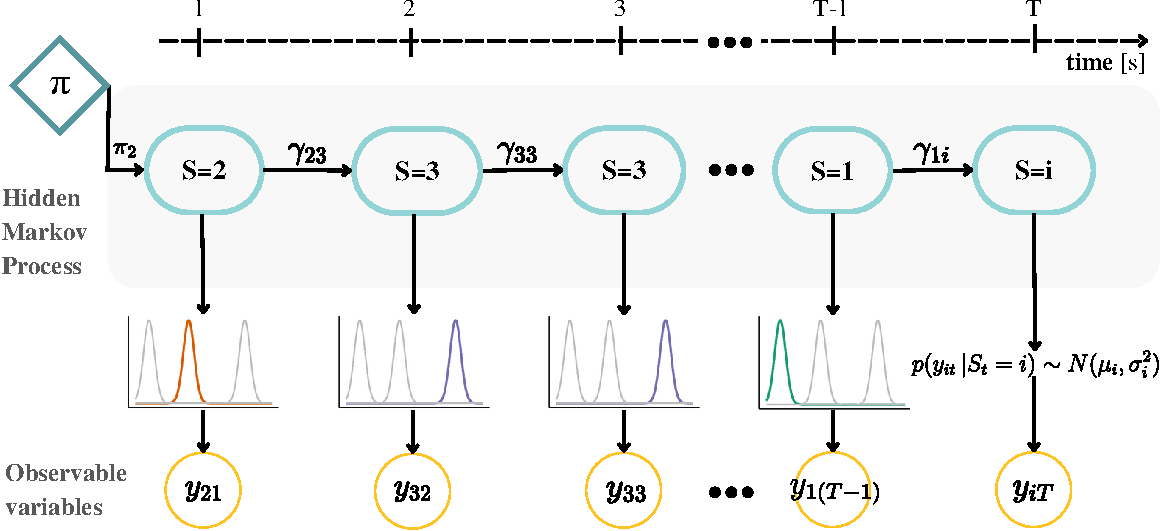
\includegraphics[width=\textwidth]{graphics/time_hmm_2.pdf}
\flushleft
\footnotesize
\justifying
The figure shows the structure of the Hidden Markov Model based on three hidden states and one normally distributed dependent variable. The model can be defined by three sets of parameters: 1) the vector $\pi$ of initial probabilities where $\pi_2$ is a probability of $S=2$ to be the initial state, 2) the TPM $\Gamma$ with $\gamma_{ij}$ for ${i,j \in \{1,2,3\}}$, and $\gamma_{23}$ represents the probability of switching from $S=2$ to $S=3$, and 3) the state-specific emission distributions of observed events $y_t$. At each point in time, the system transition to a new state, e.g., $S=3$ at $t=2$, one outcome measure $y_{32}$ is drawn from Normal emission distribution (highlighted in purple) with state-specific parameters.
 \label{hmm_fig}
\end{figure}
\section{Theoretical Background}
\subsection{Hidden Markov Model}
The Hidden Markov Model is a statistical method used to infer hidden states ${S_t \in (1,2,...,m)}$ at each time point ${t=1,.., M}$ from the observed series ${(y_1,y_t,...,y_M)}$, where $m$ is the total number of states, $y_t$ is a measurement at a given time point $t$ and $M$ is the total length of the series. The method measures the dynamics of discrete hidden states via the dynamics of the observable shifts in measurements. A detailed illustrative example of the structure of \ac{hmm} in Figure \ref{hmm_fig}. 


The \ac{hmm} is driven by two main assumptions. The first one states that all hidden states follow a Markov Process (Hidden Markov Process) meaning that the conditional probability distribution of future states depends only upon the present state at any point in time (also known as the memoryless assumption). We refer readers to Figure \ref{hmm_fig2}A where the assumption can be further inspected. In terms of probability equations, the property is defined as: 
\begin{equation}
 Pr(S_t=i \rightarrow S_{t+1}=j)=Pr(S_{t+1}=j|S_{t}=i)=\gamma_{ij}
 \label{ee1}
\end{equation}
i.e. the probability of switching from state $i$ at time point $t$ to state $j$ at $t+1$, that only depends on the previous state $i$ for all ${i,j \in (1,2,..m)}$. We call the switching probability a transition probability $\gamma_{ij}$. The matrix containing all probabilities $\gamma_{ij}$ is called the Transition Probability Matrix (TPM) $\Gamma$ and can be seen in Figure \ref{hmm_fig2}B.
The second assumption regards the inference of latent states from observed time sequences. In \ac{hmm} at each point in time $t$, one hidden state $S_t=i$ generates one observed measurement $y_t$. Note that on the first time occasion, an initial state is drawn from the initial probability $\pi$. The probability of the $y_t$ is exclusively determined by state ${S_t=i}$: 
\begin{equation}
 Pr(y_t|y_{t-1},...,y_1, \, S_t,...,S_1)=Pr(y_t|S_t=i)
 \label{e2}
\end{equation} 
and is called the emission probability. The emission probability for each state ${i\in (1,2,...,m)}$ can have any distribution, e.g, discrete or continuous, depending on the observed data character. In our research, we focus on continuous outcomes and assume normally distributed emission probability:
\begin{equation}\label{e5}
 p(y_{t}|S_t=i)\sim N(\mu_{i},\sigma^{2}_{i})
\end{equation}
where $\mu_i$ refers to the state-specific mean and $\sigma^{2}_{i}$ is the state-specific variance of the observed variable. The emission distribution can readily be extended to a $k$ number of dependent variables, each following the previous specifications. 

We also would like to point out that the \ac{hmm} presented above, is a discrete-time model. That said, the dwell times are represented by self-transition probabilities $\gamma_{ii}$, where the probability of a certain dwell time (time $d$ spent in state $S=i$) is given by the geometric distribution: ${\gamma_{ii}^{d-1}(1-\gamma_{ii})}$. In the next sections, we will present an extension of the \ac{hmm}, where the dwell time distributions are approximated with a more flexible log-normal distribution.

% In general, the \ac{hmm} can be defined by three sets of parameters: the vector $\pi$ of initial probabilities $\pi_i$, the transition probability matrix (TPM) $\Gamma$, and a set of parameters that characterize emission probability distributions ($\mu_{i}$ and $\sigma^{2}_{i}$ for all $i$).

\begin{figure}[h]
\caption{\\The Hidden Markov Process for three-state Hidden Markov Model}
\centering
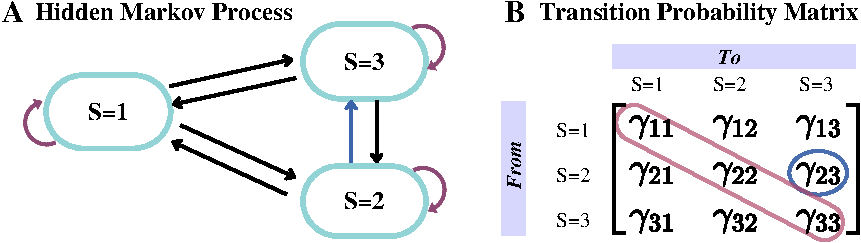
\includegraphics[width=0.8\textwidth]{graphics/time_hmm_s2.pdf}
\flushleft
\footnotesize
\justifying
Panel A: A visual representation of the Hidden Markov Process, where straight arrows represent transitions between states and curved arrows represent self-transitions. Panel B: The Transition Probability Matrix summarizing the Hidden Markov Process, where the diagonal entries are the probabilities of self-transitions and off-diagonal entries are the probabilities of transitioning between two different states. For example, $\gamma_{11}$ is the probability of remaining in the same state $S=1$ at the next time step of the process.
 \label{hmm_fig2}
\end{figure}

\subsection{The Multilevel Hidden Markov Model}
Following the work of \cite{altman_mixed_2007} we extend the \ac{hmm} to a multilevel framework by implementing subject-specific random effects. This extends the \ac{hmm} framework \linebreak to a hierarchical setting where subject-specific parameters can be estimated, allowing individual differences in underlying processes to be incorporated. In \ac{mhmm} assumptions introduced for \ac{hmm} and described with Equation \ref{ee1} and \ref{e2} remain, while the number of parameters extends by the number of added random effects. Below, we describe the \ac{mhmm} parameters' derivation process. 

The subject-specific transition probabilities $\gamma_{nij}$ are modelled from a set of multinomial logits $\alpha_{nij}$ using: 
\begin{equation}\label{e3}
 \gamma_{nij}= \frac{exp(\alpha_{nij})}{1+\sum_{s=2}^{m} exp(\alpha_{nis})}
\end{equation}
where
\begin{equation}
\label{e4}
\alpha_{nij}=\bar{\alpha}_{ij}+\epsilon_{nij} \end{equation}
for each individual ${n\in \left ( 1,..., N\right )}$, and each ${i, j\in \left \{ 1,..., m \right \}}$, where $N$ is the total number of individuals and $m$ is defined as before, with $\bar{\alpha}_{ij}$ being the (group-level) average logit for transitioning from state $i$ to state $j$, and $\epsilon_{nij}$ denotes the subject-specific deviation from the average. The individual-level random effects $\epsilon_{nij}$ follow a multivariate normal distribution with zero mean vector of length $m(m-1)$ and covariance matrix $\Sigma_{[\alpha]}$.
To ensure the identifiability of the $\Gamma$'s estimates, the numerator of the multinomial logit in Equation \ref{e3} is fixed at $1$ for $j=1$, making the transitions to the first state reference category in each row of $\Gamma$. Throughout the remainder of this text, we refer to the group-level average logit $\bar{\alpha}_{ij}$ as the TPM group-level fixed effects, and the (diagonal) variance components $\sigma^{2}_{[\alpha]ij}$ from the covariance matrix $\Sigma_{[\alpha]}$ the TPM individual-level random effects.
The subject-specific emission probability denoted as $Pr(y_{nt}|S_t=i)$ and interpreted as in Equation \ref{e2} is inferred from the Normal distribution (as in Equation \ref{e5}) with subject-specific mean $\mu_{ni}$ defined as:
\begin{equation}\label{e6}
 \mu_{ni}=\bar{\mu}_{i}+u_{ni}
\end{equation}
where for each individual ${n\in \left ( 1,..., N\right)}$ and state $i\in \left \{ 1,..., m \right \}$, $\bar{\mu}_{i}$ is the (group-level) mean of the dependent variable for each state and $u_{ni}$ denotes the individual-level deviation from the group-level mean. The $u_{ni}$ follow a normal distribution with mean 0 and variance $\sigma^{2}_{[\mu]i}$ fixed for all $i$. The variance $\sigma^{2}_{i}$ (refer to Equation \ref{e5}) of subject-specific emission distribution fixed across individuals. Throughout the remainder of this text, we refer to the group-level dependent variable mean $\bar{\mu}_{i}$ and variance $\sigma^{2}_{i}$ as the emission distribution group-level fixed effects, and the variance vectors $\sigma^{2}_{[\mu]i}$ the emission distribution individual-level random effects.

\subsection{Multilevel Explicit-Duration Hidden Markov Model}

The Explicit-Duration Hidden Markov Model  \citep[EDHMM;][]{freguson1980variable} is a more general form of the \ac{hmm}, where the memoryless assumption of the dwell times, specific to the \ac{hmm}, is relaxed. The self-transitions dictating the dwell times of each state in \ac{hmm} are redundant in \ac{edhmm}. Instead, the dwell time is explicitly derived from the set of state-specific dwell time distributions (see Figure \ref{edhmm_fig} for a detailed example of the \ac{edhmm}). Since transitions between states in the \ac{edhmm} follow the Hidden Markov Process and only self-transitions are replaced with dwell time distributions, the model assumes that latent states follow the Hidden Semi-Markov Process (see Figures \ref{edhmm_fig2}A and \ref{edhmm_fig2}B for an illustrative example of the assumption). 
\begin{figure}[]
\caption{\\The structure of the Explicit-duration Hidden Markov Model} 
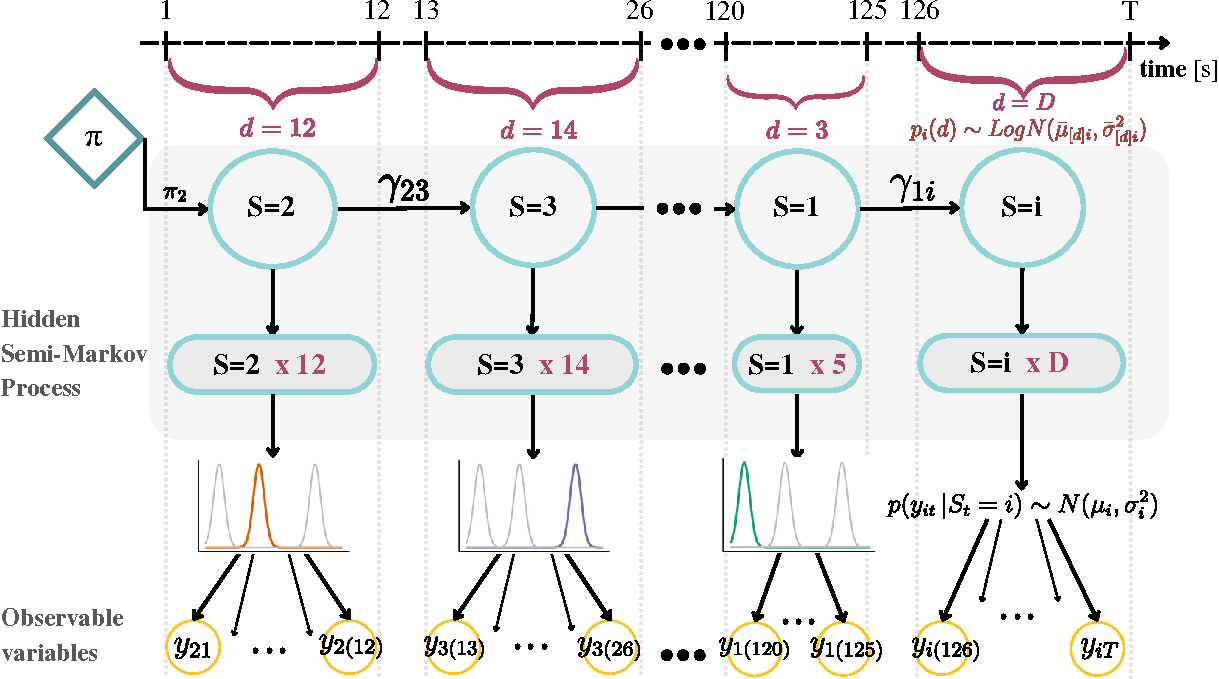
\includegraphics[width=\textwidth]{graphics/time_ed2.pdf}
 \flushleft
 \footnotesize
 \justifying
 The structure of the Explicit-duration Hidden Markov Model is based on three hidden states model and one normally distributed dependent variable. The model can be defined by four sets of parameters: 1) the vector $\pi$ of initial probabilities where $\pi_2$ is a probability of $S=2$ to be the initial state, 2) the TPM $\Gamma$ with $\gamma_{ij}$ for all $i\neq j$, and $\gamma_{23}$ represent the probability of switching from $S=2$ to $S=3$, 3) the state-specific dwell time distributions, in this case, the log-normal, and 4) the state-dependent emission distributions of observed events $y_t$ generated from hidden states. The dwell-times $d$ are drawn from the log-normal distributions each time the system transition to a new state $S$ i.e. when at time point $t=13$ latent state switch from S=2 to S=3 the dwell-time d=14 is drawn from the log-normal distribution with parameters specific to $S=3$. 
\label{edhmm_fig}
\end{figure}

\begin{figure}
\centering
\caption{\\The Hidden Semi-Markov Process for the three-state }
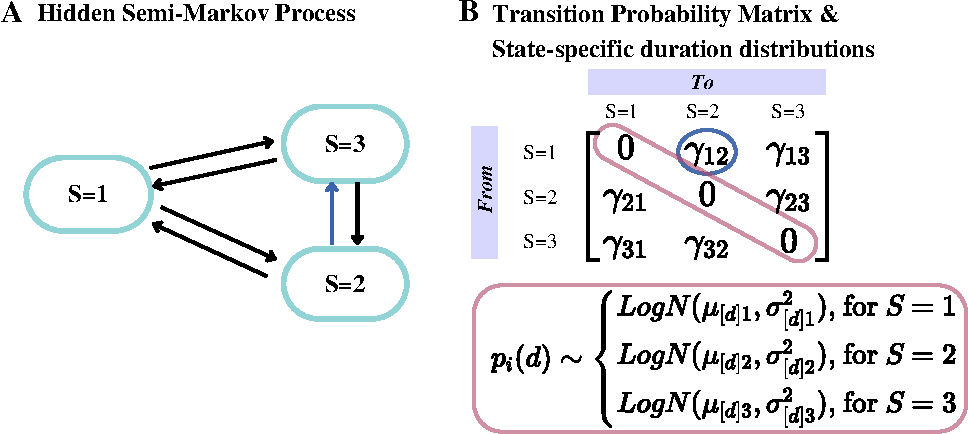
\includegraphics[width=0.85\textwidth]{graphics/time_edhmm_s2.pdf}
\flushleft
\footnotesize
\justifying
Panel A: A visual representation of the Semi-Markov Process. The straight arrows represent transitions between states. In comparison to Figure \ref{hmm_fig2}A self-transitions (curved arrows Figure \ref{hmm_fig2}A) are redundant in EDHMM. Panel B: The Transition Probability Matrix of the process, where the diagonal entries equal to $0$ and off-diagonal entries are the probabilities of transitioning between two different states e.g., $\gamma_{13}$ is the probability of transitioning from state $S=1$ to state $S=2$ at the next time step of the process. Instead of diagonal entries in the TPM, the set of dwell-time probabilities is assumed by the EHMM (outlined in red, below TPM).
 \label{edhmm_fig2}
\end{figure}
\newpage
In the Semi-Markov Process, the transition probabilities depend on a previous state ${S_{t}=i}$, as in \ac{hmm}(and \ac{mhmm}), and its duration $d_{S_{t}=i}$:
\begin{equation}
 Pr(S_t=i \rightarrow S_{t+1}=j)=Pr(S_{t+1}=j|S_{t}=i,d_{S_{t}=i})=\gamma_{ij} \\\text{, for } i\neq j,
\end{equation}
where the $d_{S_{t}=i}$ is a random integer from the range ${\left [ 1, d_{max} \right ]}$, and $d_{max}$ is the maximum allowable state duration.

The subject-specific dwell time probability for \ac{medhmm} is defined as:
\begin{equation}
\label{eq5}
 p_{i}(d_n)=Pr(S_{t+1:t+d_n]}=i|S_{[t+1:}=i)\text{, with} \sum^{d_{max}}_{d_n=1}p_{i}(d_n)=1,
\end{equation}
i.e. the probability that a state $i$ starts exactly at time ${t + 1}$ and ends at exactly ${t + d_n}$. The probabilities for all possible subject-specific state durations $d_n$ must sum up to $1$ for each state $i$. Note that we focused on the right-censored formulation here \citep{Guédon_2007}, which means that in the last visited state, the duration is estimated to be no longer than $M-t$, where $t$ is the current time point of observation and $M$ is the total length of the observation sequence.

In order to make the likelihood computation feasible, we obtain the probability of state-dependent duration $d_n$ only for whole units of time $t$. It implies that the state-specific dwell time distribution $p_i(d_n)$ is discrete. However, in case one assumes a parametric distribution, the $p_{i}(d_n)$ can be defined by any imposed distribution. To ease the burden of likelihood computation while maintaining flexibility in dwell time estimation in the current study, we consider $p_{i}(d_n)$ log-normally distributed. In addition, the distribution was most feasible to use in a Bayesian context that we intend to apply. \newpage That said, we can represent the $p_{i}(d_{n})$ as:
\begin{equation}
 p_{i}(d_{n})\sim LogNormal\left ( \mu_{[d]ni}, \bar{\sigma}^2_{[d]i} \right )
\end{equation}
with 
\begin{equation}
\mu_{[d]ni}=\bar{\mu}_{[d]i}+q_{ni}
\end{equation}
where, for each individual ${n\in \left ( 1,..., N\right )}$ and state ${i\in \left \{ 1,..., m \right \}}$, $\mu_{[d]ni}$ is the subject-specific log-mean and $\bar{\sigma}^2_{[d]i}$ the group-level log-variance. The subject-specific deviations from the group-level log-mean $\bar{\mu}_{[d]i}$ are denoted as $q_{ni}$ and normally distributed with mean zero and variance $\sigma^{2}_{[d]i}$, fixed across all individuals $n$. Furthermore, $\mu_{[d]i}$ and $\mu_{[d]ni}$ are means of the log-transformed durations, and $\exp{(\mu_{[d]i})}$, as well as, $\exp{(\mu_{[d]ni})}$ are medians of the untransformed durations. That said, for more intuitive descriptions, we will use the medians of the dwell time distributions ($\exp{(\mu_{[d]i})}$ and $\exp{(\mu_{n[d]i})}$) to describe the expected state durations and from this point onwards we will refer to it as mean/expected state duration or dwell time.

Since self-transitions are not estimated in the \ac{medhmm}, the $\Gamma$ is defined such that the diagonal entries $\gamma_{nij}$ for ${i=j}$ and ${i,j\in(1,2,...,m)}$ are equal to $0$. The off-diagonal entries of $\Gamma$ are derived similarly to the \ac{mhmm} presented in Section $2.2$ with Equation \ref{e3} adjusted such that transitions to the first state with non-zero probability, are the reference categories in each row of the TPM. Upon transitioning to a state $i$, in \ac{medhmm} a sequence of observations ${y_t, y_{t+1},...,y_{t+d_n}}$ of length $d_n$ is emitted from the emission distribution (refer to Equation \ref{e2}-3 and Equation \ref{e6}).

Note that in both \ac{mhmm} and \ac{medhmm} models, the number of states $m$ must be determined a priori by the researcher. Choosing the number of hidden states without a theoretical justification becomes a model selection problem for which standard criteria can be applied (e.g., Akaike information criteria (AIC), the Bayesian information criterion (BIC) etc.). For a detailed discussion on the issue, we refer the reader to \cite{de_haan_rietdijk_use_2017}. 

%\subsubsection*{The choice of the dwell time distribution}
%There are many options for dwell time distribution that researchers have successfully implemented. The two main determinants of appropriate dwell time are the subject of analysis and the compatibility of the proposed distribution with estimation algorithms. The Poisson duration distribution was used to model duration in speech recognition by \citep{1168477}. The Inverse gamma duration distribution has been used by \cite{Nagaraja_1996} to model patients’ staying time in the hospital. The Coxian distribution has been applied by \cite{1595592} to the task of recognizing activities of daily living in a smart house environment. In chapter 5 of \cite{Emm_Th} Log-normal duration distribution has been assumed to capture the movement stages of mice behaviours. In the study, we chose the Log-normal distribution as the distribution of the state-dependent duration probabilities, since it is most feasible to use in a Bayesian context that we intend to apply. 

% \begin{equation}
% p_i(d)\sim LogNormal(\mu_{[d]i},\sigma^2_{[d]i})
% \end{equation}
% where $\mu_{[d]i}$, denotes the logmean (i.e., the mean of the log-transformed durations) and $\exp{(\mu_{[d]i})}$ is the median of the (untransformed) durations, and $\sigma^2_{[d]i}$ denotes the variance in the log-transformed durations. As the median duration
% is more intuitive to interpret than the mean of the log-transformed durations, we will
% often use the median duration, denoted by $\exp{(\mu_{[d]i})}$, to describe the state durations.

% All in all, the \ac{edhmm} can be defined by four sets of parameters: the vector $\pi$ of initial probabilities $\pi_i$, TPM $\Gamma$, the set of parameters of state-dependent dwell time distributions and the set of parameters of the state-dependent probability distribution of observed events $y_t$.






% \subsection{Hidden Markov Model and Explicit-duration Hidden Markov Model in multilevel framework} 

% Traditionally, \ac{hmm}s, as well as \ac{edhmm}s, were applied to a time-series data sequence such as speech or written text (eg. \cite{Rabiner_1989} [\ac{hmm}], \cite{freguson1980variable} [\ac{edhmm}]). Behavioural and social data, however, are frequently collected as a series of observations (\ac{ild}) from multiple individuals. The collected data often resembles a hierarchical structure (add citation), where time-series observations are nested within individuals. Considering the extra complexity of the data, a few fitting data approaches have been taken to exploit the information effectively. (now I will present the 3 approaches and express a favour towards the last one. I'm editing the part now). One way is to fit models on pooled data, not considering possible correlations within the observations that are due to the hierarchical structure of the data. In that way, we obtain average results across the investigated group. We ignore the individual homogeneity of observation and heterogeneity between participants but we get average estimates of the sample parameters. On the other hand, for each participant, we can fit a separate hidden Markov Model (Mixture Hidden Markov Model). The method has been used in many publications (e.g ... \cite{visser_mixture_2022}). The Mixture Hidden Markov Model allow for the investigation of trends in sequences characteristic of the subject. However, it is highly computationally intensive and doesn't give us a chance to refer the individual patient's dynamics to the group-level estimates. Note that multiple hidden Markov models might result in best models that vary in terms of the number of states for example. It is not correct since the aim of a study is usually to compare participants on a given fixed condition. Finally, one can apply the \ac{hmm} or \ac{hsmm} in a Multilevel framework (short \ac{mhmm} and \ac{mhsmm}). \ac{mhmm}s and \ac{mhsmm}s that take into account both the homogeneity of observations between subjects and heterogeneity of individuals, while treating it all as the same system. That way, we are able to model the complex data system under one model. In the multilevel framework, we account for individual variability by introducing individual random effects, which can be seen as individual deviations to fixed group-level estimates of parameters of the \ac{hmm} and \ac{edhmm}.


%Note that $\mu_{[d]i}$ and $\mu_{n[d]i}$ are means of the log-transformed durations, and $\exp{(\mu_{[d]i})}$ and $\exp{(\mu_{n[d]i})}$ are medians of the (untransformed) durations. That said, for more intuitive descriptions, we will often use the medians of durations ($\exp{(\mu_{[d]i})}$ and $\exp{(\mu_{n[d]i})}$) to describe the state durations.


% A potential issue that may arise during Bayesian estimation of the \ac{mhmm} or \ac{edhmm} is what has been referred to as label switching \citep{Celeux_Hurn_Robert_2000}.The most common way to prevent label switching has been defining appropriate starting values and having well-defined and distinct (not overlapping) state distributions. 

% The Bayesian approach eliminates the need for numerical integration and enables interval estimation as a direct product of the estimation routine. Simulation-based methods, such as the Markov chain Monte Carlo approach [20] including the Metropolis-Hasting algorithm [21, 22] and the Gibbs sampler [23], make the Bayesian approach relatively easily adaptable to complex latent variable models that are more difficult to fit in the frequentist setting.

% There is no straightforward criterion for model fit or model selection that can be used to choose the number of latent states when that number is not known a priori. Researchers working in the frequentist framework often use the Akaike Information Criterion (AIC; Akaike, 1974) or Bayesian Information Criterion (BIC; Schwarz, 1978) for model comparison and for choosing the number of latent states. Other methods used has been DIC Bayes Factor 
% In the Bayesian framework, the exact Bayes factor for model comparison is difficult to implement, and both exact and approximate Bayes Factors (such as the BIC approximation, cf. Kass & Raftery, 1995) yield results that depend on a specific prior distribution (Frühwirth-Schnatter, 2006). Another commonly used criterion is the Deviance Information Criterion (DIC; Spiegelhalter, Best, Carlin, & Van Der Linde, 2002), but there is no consensus on the right way to define the DIC for multilevel models (Celeux, Forbes, Robert, & Titterington, 2006).
% A potential issue that may arise during Bayesian estimation of the \ac{mhmm} or \ac{edhmm} is what has been referred to as label switching (\cite{Celeux_Hurn_Robert_2000}. The problem is caused due to the fact that the likelihood of a Bayesian multilevel model could be invariant to permutations of the values, “labels”, of the discrete latent variable. This may lead to uninterpretable results Hence we should always make an effort to prevent it from happening. The most common way to prevent label switching has been defining appropriate starting values and having well-defined and distinct (not overlapping) state distributions which we made sure to implement on our study.

\section{Simulation Study}
%In the introduction, we pointed out that the \ac{mhmm} assumption of the dwell times following geometric distribution is far from realistic in some applications. Hence, we proposed \ac{medhmm}, a novel approach that enables researchers to model a flexible range of state durations. The model incorporates dedicated dwell time distributions, which improves model interpretability and dwell time estimation \citep{Yu_2010}. However, the \ac{medhmm} comes at the expense of increased complexity, which leads to longer computation times and may require more resources (e.g. observations per subject). 
The purpose of the Monte Carlo simulation study was to compare the performance of the \ac{medhmm} and \ac{mhmm}. We simulated data from the Multilevel Explicit Duration Hidden Markov model using a full factorial design, varying three factors: 1) the number of hidden states, 2) the number of observations, and 3) the mean dwell time. Also, we included one extra simulation scenario to assess the effect of varying across-stats dwell times. We chose levels of each factor based on the \ac{mhmm} literature and summarized them in Table \ref{tb1}.\\ 

\begin{table}[h]

\caption{The summary of simulation study levels with three varying factors*}\label{tb1}
\begin{tabular}{c|c|c} 
\hline
Number of states ($m$)& Sample size ($N_{obs}$) & Mean dwell time ($d$) \\ 
\hline
3 & 200 & 1.4 \\
4 & 500 & 3.5 \\
 & 1000 & 19.5 \\
 & & 99.5 \\
\hline
3 & 500 & \{3.5, 19.5, 99.5\} \\
\hline
\end{tabular}
\flushleft
\footnotesize
\justifying
* The first four rows shows the simulation scenario levels to which we applied the full\\factorial design.
The last row includes the specifications of the additional simulation\\ scenario with varying across states dwell time. 
\end{table}

\subsection{Levels of the simulation study}
\subsubsection*{Number of states}
In order to assess how the number of parameters to infer influences the bias in its estimates, we considered two levels for a total number of states ${m \in \{3,4\}}$. With each level, the number of parameters increases quadratically with the number of states, i.e., the total number of parameters to estimate for both models is $m^2(N+1)$, where N is the number of individuals. The choices were made based on literature, which revealed that \ac{mhmm}s were typically fitted to three hidden states in \cite{maruotti_multilevel_2022}, \cite{Long_Tang_Wang_Jiang_2019}, \cite{de_haan_rietdijk_use_2017} and \cite{shirley_hidden_2010} and usually, not more than four hidden states \citep[see][]{Schafer_Wikle_VonBank_Ballard_Weegman_2020,inaba_mixed_2017}. 
%The two-state model was not considered in this simulation study due to its specific character in light of MEDHMM (the probabilities to transmit to any other state is fixed to 1 and the switches between states are purely dictated by the dwell time of a given state. 
\subsubsection*{Sample Size}
Based on the \ac{mhmm} literature, we decided to fix the number of individuals to ${N_{ind}=80}$, which indicated a median number of participants in studies that utilised \ac{ild} \citep[][]{altman_mixed_2007,Schliehe_Diecks_Kappeler_Langrock_2012,Schafer_Wikle_VonBank_Ballard_Weegman_2020, de_haan_rietdijk_use_2017,inaba_mixed_2017}. The levels of observations we set to ${N_{obs}\in \{200, 500, 1000\}}$. The literature included time series sample sizes ranging from $24$ in \cite{altman_mixed_2007} to $7257$ in \cite{inaba_mixed_2017}. However, we perceived the $24$ observations as not enough in the spirit of modern \ac{ild} designs and set the lower bound to $200$. The upper bound we chose to be ${N_{obs}=1000}$ since in behavioural settings this amount of observations per individual is seen as large.
\subsubsection*{Mean dwell time}
Since we based the design of the simulation study on the MHMM literature, we translated the information encoded in the self-transition probabilities of the TPM of MHMM into the expected dwell times that further were transformed to log-means and log-variances of the log-normal dwell time distribution (refer to next section for the details of transformation). The self-transition probabilities according to the reviewed literature including \cite{altman_mixed_2007,Schliehe_Diecks_Kappeler_Langrock_2012, de_haan_rietdijk_use_2017,Raffa_Dubin_2015,inaba_mixed_2017}, and \cite{Schafer_Wikle_VonBank_Ballard_Weegman_2020} were generally in range $\gamma_{ii}\in\{0.5-0.95\}$. We considered four levels of self-transition probabilities ${\gamma_{ii} \in \{0.5, 0.75, 0.95, 0.99\}}$, which correspondingly can be interpreted as low, medium, and high and very high state persistence and the mean dwell times that follow from them are ${d\in \{1.4,3.5,19.5,99.5\}}$. Note that the listed $d$ expected state durations were used in the full factorial design, where they were constant across states. The additional scenario involved ${d_a\in \{3.5,19.5,99.5\}}$ where each $d_a$ represented a different state-specific mean duration. 

% \begin{table}
% \tbl{Example of a table showing that its caption is as wide as
% the table itself and justified.}
% {\begin{tabular}{lcccccc} \toprule
% & \multicolumn{2}{l}{Conditions} \\ \cmidrule{2-4}
% Paper & States & Subjects & Occasions\\ \midrule
% \citep{maruotti_multilevel_2022}& 3 & 474 & 10 \\
% \citep{altman_mixed_2007}& - & 30 & 1-24 \\
% \citep{shirley_hidden_2010}& 3 & 240 & 168 \\
% \citep{de_haan_rietdijk_use_2017} &3 & 149 & 539 \\
% \citep{de_haan_rietdijk_use_2017} & 2 & 224 & 56 \\
% \citep{inaba_mixed_2017} & 2 & 89 & 20 \\
% \citep{Schliehe_Diecks_Kappeler_Langrock_2012} & 2 & 59 & 26\\
% \citep{Schafer_Wikle_VonBank_Ballard_Weegman_2020} & 4 & 50-100 & 5 \\
% \citep{Long_Tang_Wang_Jiang_2019} & 3 & 133 & 1064 \\
% \citep{inaba_mixed_2017} & 4 & - & 7257 \\ \bottomrule
% \end{tabular}}
% \label{Multilevel Hidden Markov models studies}
% \end{table}


\subsection{Data generation mechanism }
We simulated $128$ datasets from each of the $24$ scenarios using the factorial design on the parameters listed in Table \ref{tb1}. One additional scenario has been included to inspect the performance of the three-state model with varying between states dwell times. To ensure the stability of results and prevent convergence failures such as label switching, data were generated with two univariate normally distributed dependent variables with group-level means ${\bar{\mu}_{1i},\bar{\mu}_{2i}\in \{10-98\}}$ and variances ${\sigma_{1i}^2 \in \{20-150\}}$ for the first variable and ${\sigma_{2i}^2 \in \{25-187.5\}}$ for the second one (see Figure \ref{em_ds} in Appendix A for more details). In general, the parameters of emission distributions have been chosen such that the overlap proportion between subsequent state-dependent distributions was equal to $0.10$ for the first and $0.14-0.15$ for the second dependent variable. Random effects $u_{ni}$ were normally distributed with mean $0$ and variance ${\sigma^2_{[\mu]1i},\sigma^2_{[\mu]2i}=9}$ for both variables.

The dwell time probability was log-normally distributed (see Figure \ref{log_ds} in Appendix A for an illustration of the assumed distribution). The expected dwell times (medians of log-normal distributions) were set to ${d\in \{1.4,3.5,19.5,99.5\}}$ and obtained via transforming the self-transition probabilities ${\gamma_{ii} \in \{0.5, 0.75, 0.95, 0.99\}}$ using the formula\footnote{The expected state duration when the exponential distribution is assumed to be an approximation of the geometrical dwell time distribution for \ac{mhmm}.}: ${d=1/-\log(\gamma_{ii})}$. In order to get the log-mean and log-variance of the target distribution, we calculated ${\bar{\mu}_{[d]i}}$ by taking the logarithm of the expected dwell times $log(d)$. The log-variance ${\bar{\sigma}^2_{[d]i}}$ has been set such that the standard deviation of each dwell time distribution was equal to a third of the $d$ for, ${d\in \{1.4,3.5,19.5\}}$ except from when $d=99.5$ for which the standard deviation was a quarter of the value. In the result, the log-variances were equal ${\sigma^2_{[d\in \{1.4,3.5,19.5\}]i}}=0.096$ and ${\sigma^2_{[d=99.5]i}}=0.057$. The random effects $q_{[d]ni}$ were normally distributed, with mean $0$ and variance $\sigma^{2}_{[\bar{d}]i}=0.2$ that was common to all $d$. 

The TPM parameters were derived from multinomial logits where the off-diagonal entries were set so that there is an equal chance of transitioning to another state (e.g., the first row of TPM for $m=3$ was $\gamma_{1j}=[0 \,\,\, 0.5 \,\,\, 0.5]$). The individual-random effects of the transition distribution were normally
distributed with mean $0$ and variance ranging ${\sigma^2_{[\alpha]nij}=0.17}$ on the logit scale,
which translates to standard deviations on the off-diagonal entries in TPM ${\sigma_{\gamma_{nij}}=0.1}$, for ${i\neq j}$ on the probability scale. For simplicity, we will call the set of multinomial logits, the gamma distribution and the set of transformed logits representing the transition probabilities the transition distribution. The simulation script can be accessed via the link in the Supplementary Materials. 

\subsection{Model fitting}
Simulating data and fitting models was done in the statistical software R (R Core Team, 2022) and executed with the use of the Dutch National Supercomputer Snellius. We used developer versions of the \emph{mHMMbayes} package\footnote{The GitHub repository containing the \emph{mHMMbayes} package source code used in this analysis can be found under the following link: \url{https://github.com/emmekeaarts/mHMMbayes/tree/continuous-emiss}} \citep{mHMMbayespackage} and developer version of the \emph{medHMM} package\footnote{The GitHub repository containing the \emph{medHMM} package source code used in this analysis can be found under the following link: \url{https://github.com/emmekeaarts/medHMM/tree/dev}}, tailored accordingly to \ac{mhmm}s and \ac{medhmm}s for continuous dependent variables. Packages employ Bayesian estimation methods \citep{Emm_Th,Scott_2002} and forward-backwards algorithms to infer parameters \citep{Scott_2002}. 

As for, the \ac{mhmm} the (forward) probabilities of each state at every time point are calculated given the observed data. The hidden state sequence is then sampled from their full conditional posteriors in a backward pass given the (current) parameters of the model\footnote{For a detailed description of the estimation algorithm, see: \url{https://cran.rproject.org/web/packages\\/mHMMbayes/vignettes/estimation-mhmm.pdf}}. Based on the sampled hidden state sequence, the parameter estimates are updated by sampling them from their full conditional posteriors using either a Gibbs or a Random Walk Metropolis-Hastings step. In the case of \ac{medhmm}, the forward probabilities are calculated for each state and each duration $d$ in set $d\in[1,2,..,d_{max}]$. Then, the hidden states and their discrete durations are drawn from their full conditional posteriors in a backward pass, forming the hidden state sequence, and the rest follows. In this study, the $d_{max}$ was chosen such that it covered at least $95\%$ of the state persistence on different simulation levels (low, medium, high and very high) and is in the range $d_{max}\in\{100-600\}$. Besides that, the Bayesian approach to parameter estimation enables flexible parameter inference while avoiding the direct computation of complex likelihoods \citep{Frühwirth-Schnatter_2001,Scott_2002}. The approach has been shown to outperform other non-Bayesian methods in terms of computing speed \citep{Rydén_2008} and provides direct estimates for the fixed and random effects in the multilevel model. Furthermore, valuable by-products are produced in the inference process such as posterior standard deviations, credible intervals, or local decoding, which identifies the most probable state out of a series of discrete hidden states at each time point. 

We used $4000$ MCMC iterations to train both \ac{mhmm} and \ac{medhmm} and dropped the first $2000$ (burn-in) to reduce the influence of the starting values on the model convergence \citep{plummer2006coda}.
For emission and dwell time distributions, we used only uninformative and weakly informative hyper-priors that can be found in Table \ref{Ap_emiss_hp} and Table \ref{Ap_dwell_hp} in Appendix A. We used provided by software default hyper-priors for transition distribution that were uninformative and can be found in vignette of the \emph{mHMMbayes} \linebreak (Footnote 4, p. 11). In order to check the convergence, we fitted 5 randomly chosen out of 128 simulated datasets to both \ac{mhmm} and \ac{medhmm} with two additional chains specified with randomized starting values. The convergence of the group-level parameters (fixed effects) was assessed with the multivariate potential scale reduction factor \citep{Brooks_Gelman_1998} with a cut-off of ${\text{R} < 1.2}$ and inspecting trace plots of the parameters visually.

We inspected the group-level parameters of the emission, transition, and dwell time distributions with bias, precision, and coverage. Medians of the Bayesian posterior distributions of group-level parameters were used as point estimates. The differences between posterior medians and assumed true values were used as bias indicators. Relative percentage bias was reported to evaluate the size of the bias due to undercoverage with respect to the true unknown parameter to estimate. The relative bias of $5\%$ or less was considered acceptable. Additionally, the MHMM transition probability matrix (TPM) parameters were reported in two ways: 1) the direct TPM estimates from the MHMM algorithm, and 2) adjusted TPM such that the diagonal entries were set to 0. Since the true TPM probabilities were always balanced (the probability to switch to a different state was equal), the average across TMP entries absolute relative bias was reported. We also compared the expected dwell times for the MEDHMM (medians of the log-normal distribution) and MHMM (expected duration based on the self-transitions probabilities calculated using formula $1/-log(\gamma_{ii})$) and reported the average absolute bias for them. Note that average absolute bias measures were only reported for full the factorial simulation, excluding the additional scenario. 

The empirical standard errors were calculated and reported as the precision measure. The $95\%$ central credible intervals were computed as indications of the uncertainty about the parameters \citep{Lynch_2007}. Moreover, the coverage of estimates was assessed by the ratio of times the $95\%$ central credible intervals of model estimates overlap their true values. Coverage of $92\%$ and above was considered acceptable. The average proportion of hidden states correctly assigned by the local decoding \citep{Scott_2002}, as well as the average proportion of instances in which the decoding probability of the true state was at least $0.2$, were used to assess model performance for individual-level inference. The $\kappa$ statistic was used to control for the expected classification accuracy due to random chance \citep{Cohen_1960}.
The full reproducible code for the analysis is available in Supplementary Materials.

\subsection{Results}
In this section, we present the results of our simulation study, which aimed to compare the performances of MHMM and the newly introduced MEDHMM. The simulated data has been developed based on behavioural research conducted on continuous, intensive longitudinal data (mentioned in Section 3.1). We start with reporting the convergence performance for both models. Then, we describe the result for group-level estimates of emission distribution, transition probabilities and dwell time distribution parameters. Lastly, we report the state decoding performance, including empirically defined dwell times and the number of state switches. The additional scenario with varying dwell times was discussed in Section 3.4.6. All results\footnote{Two simulation scenarios for four-state MEDHMM (i.e., $d=3.5$ \& $500$ observations scenario and $d=99.5$ \& $1000$ observations scenario) were not included in the current manuscript because due to unstable Snellius infrastructure and reoccurring maintenance during last two weeks before submission, the MEDHMM scenarios did not manage to run. The results for the missing scenarios will be included as soon as the Snellius infrastructure will resume. The updated version of the manuscript will be uploaded to the research repository linked in Supplementary Materials.} are available for detailed inspection in Table \ref{tgr2_1}-\ref{mixed_sim} in Appendix D, and the most important results were described in the text below. 

\subsubsection{Convergence}
Overall, parameter convergence was achieved for group-level parameters in $100\%$ of MHMM assessed scenarios with the average potential scale reduction parameter $R \in \{1-1.1\}$. In MEDHMM the convergence was reached in $100\%$ of assessed three-states scenarios with $R=1$ for all group-level parameters. The major convergence issues occurred for MEDHMM in four-state scenarios assuming short dwell times ($d=1.4$ and $d=3.5$) for which only $87.5\%$ scenarios reached convergence. We would like to point out that in any case, all five considered MEDHMMs resulted in failure to converge. The model fitting didn't encounter any issues except 3 out of 128 simulated datasets in 2 scenarios fitted to MEDHMM which resulted in model execution failure due to overflow/underflow issues. The difference in available results was minimal and should not impact the Monte Carlo standard error. Hence, the MAP results were reported based on 125 simulated datasets for the explained 2 scenarios and on 128 simulated scenarios for the rest.  All trace plots can be found under the link listed in Supplementary Materials.


\subsubsection{Emission distributions}
%Bias The bias, precision, and coverage results were comparable in their magnitudes for both dependent variables. 
\emph{Bias}     In general, the MHMM performed better in recovering the means of the emission distributions in scenarios with shorter state durations (i.e., $d=1.4$ and $d=3.5$). The estimates of the means in MEDHMM were unsatisfactory for the $d=1.4$ scenarios and became closer to the truth as the assumed dwell time started increasing. Figure \ref{mubias} shows the relative bias (\% bias) of emission distribution means for two models and different simulation scenarios. For the shortest state duration scenarios, the MEDHMM overestimated smaller values and underestimated larger emission mean values, which resulted in \% bias ranging from $-43.7\%$ to $229.6\%$ in d=1.4 and from $-8.3\%$ to $30.7\%$ in d=3.5 for two dependent variables combined. The MHMM mean estimates were overestimated for the shorter dwell times, however, the bias values were between $-0.33\%$ and $1.74\%$. The relative bias in the emission distribution means was smaller than $5\%$ in $60\%$ cases for the MEDHMM and in $100\%$ for the MHMM. In addition, relative bias was less than $5\%$ for $100\%$ of means parameters for $d=19.5$ and $d=99.5$ for both models independently of the state number assumed and the observation length.
Variance components of the emission distribution were overestimated by both models. Larger deviations from the truth were present for MEDHMM in shorter dwell time scenarios, with bias from $214.6\%$-$2414.1\%$ when $d=1.4$ and from $19.3\%$-$318.9\%$ when $d=3.5$. The range of MEDHMM bias in variance estimates decreased noticeably for longer duration scenarios and ranged from $10.8\%$ to $37.4\%$ when d=$19.5$ and between $8.5\%$ and $37.6\%$ when $d=99.5$. The MHMM bias results for the variances ranged from $10.6\%$-$40.0\%$ and were stable across varying simulation scenarios. 

\emph{Precision}  The empirical standard deviation (ESE) of the all-group level parameters for MEDHMM was highly varying across observation length and state scenarios, especially for shorter dwell times (see Figure \ref{prec_emiss} in Appendix B). For MEDHMM within longer dwell time scenarios, the ESE values were similar across parameters and comparable to the ESE values for MHMM. For MHMM, the ESE for emission distribution group-level parameters were less prone to changes with varying simulation conditions and were between $0.55$ and $0.98$ for emission means and between $1.54$ and
$10.01$ for emission variances, while for the MEDHMM those ranges were, accordingly ${0.5-2.6}$, and ${1.6- 51.3}$. On average, the ESE values for the parameters were larger for the shorter observation lengths and smaller for the longer series lengths. 

\emph{Coverage}  The coverage of the group-level means is presented in Figure \ref{emiss_mu_cov} in the Appendix and indicates that the coverage of the parameters was above $92\%$ for $100\%$ of instances for MHMM and only above $92\%$ for MEDHMM in $53\%$ of instances. However, for longer dwell time scenarios, the coverage was acceptable in $100\%$ of the mean parameters when the dwell time assumed was $d=99.5$. The coverage for the variance component was poor, with a maximum value of $35.2\%$ for MEDHMM and $10.94\%$ for MHMM.  

\begin{figure}
\caption{\\Emission distribution means: \% Bias}
    \centering
    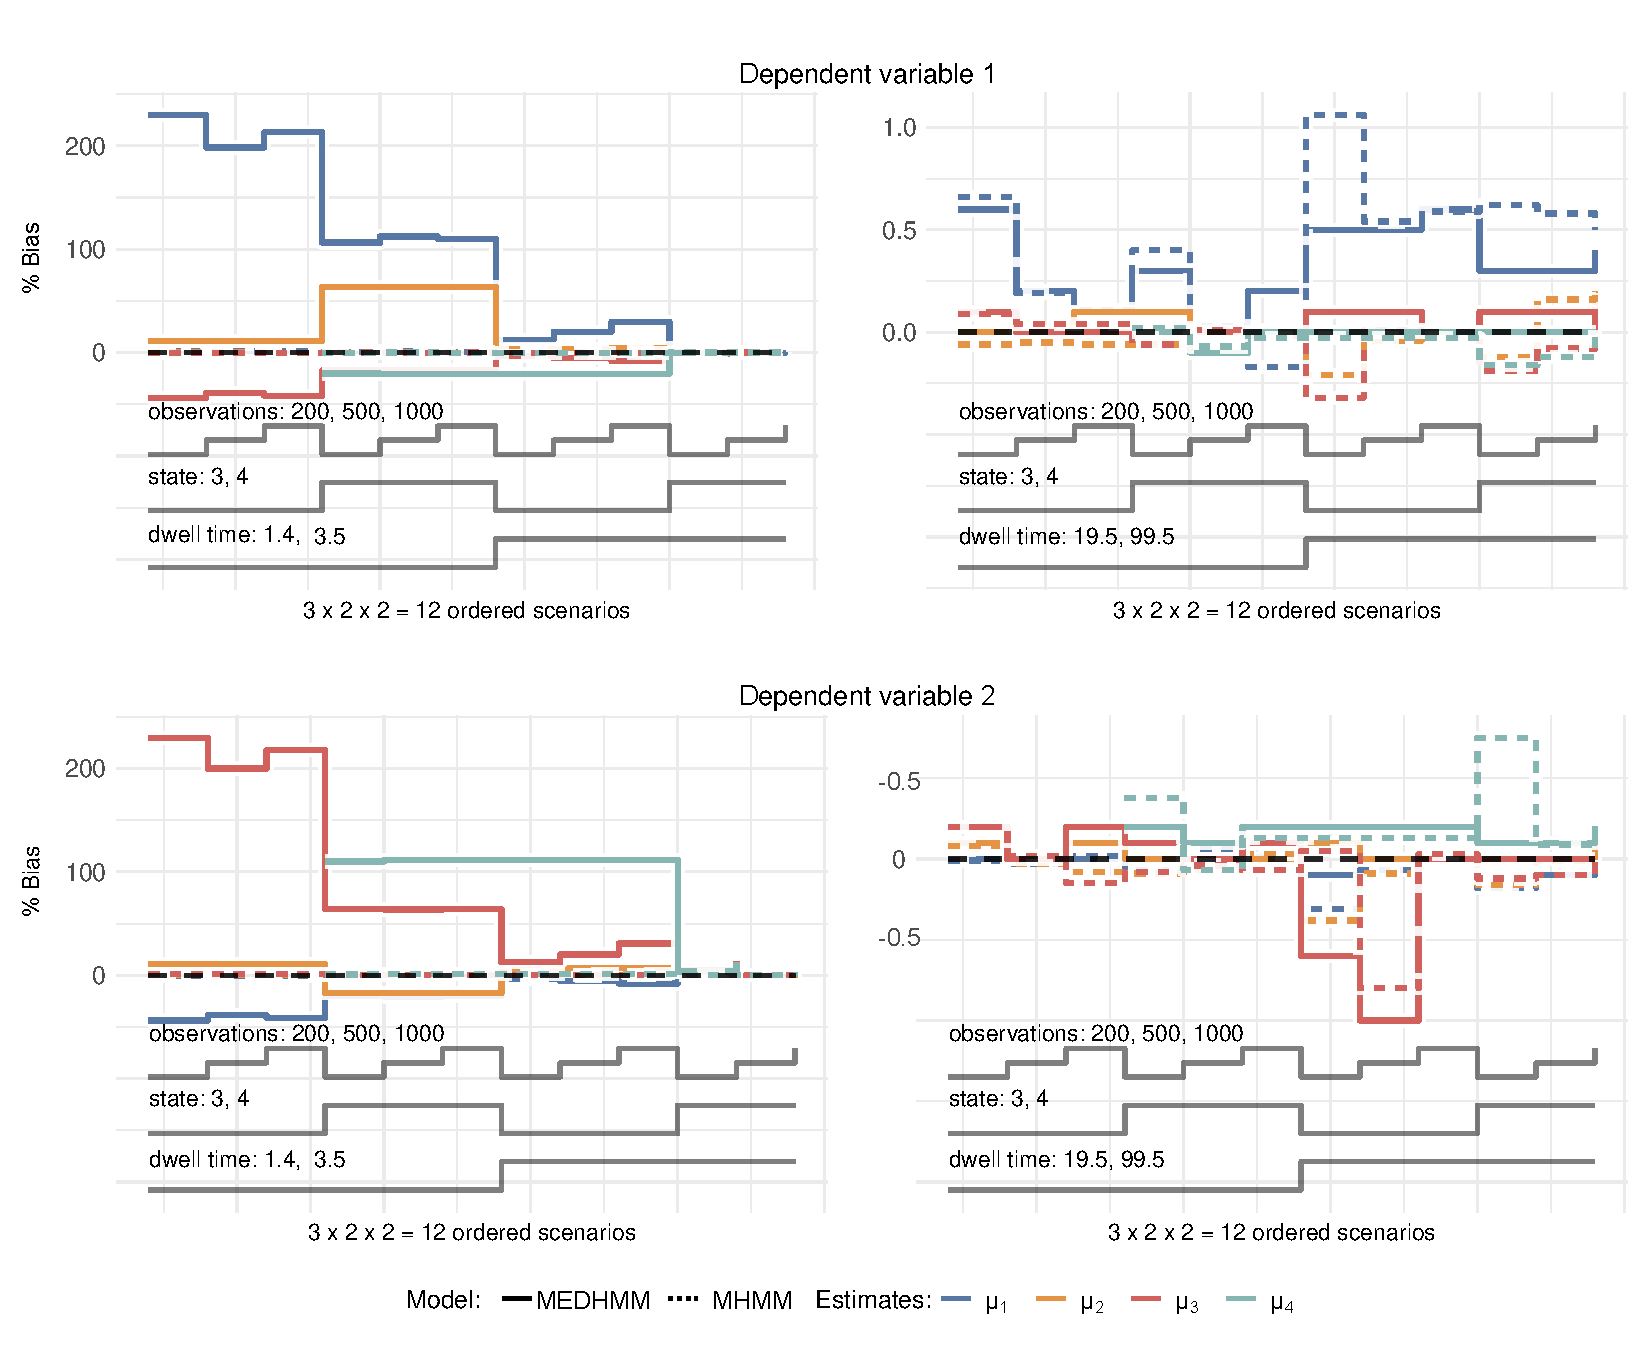
\includegraphics[width=\textwidth]{graphics/emiss_dep_bias2.pdf}
    \flushleft
    \footnotesize
    \justifying
    Plots illustrate the relative bias (\% Bias) of each emission distribution mean for every simulation scenario (note that the additional scenario with varying dwell time is omitted). The plots for each of the dependent variables are split onto two plots representing (from left) short state durations and longer state durations with dwell time $d\in \{1.4, 3.5\}$ for the left plot and $d\in \{19.5, 99.5\}$ for the right plot. Each colour represents the state-specific emission mean parameters, and line type is the model indicator.
    \label{mubias}
\end{figure}



\subsubsection{Transition distribution}
Overall, the performance of MEDHMM for the group-level transition distribution parameters worked better in terms of bias and coverage of the true parameters in comparison to the MHMM. \\
\emph{Bias}     The MEDHMM bias in TPM parameter estimates was below $5\%$ in $66\%$ of scenarios. The bias values for MEDHMM were influenced by the number of observations, states and dwell time assumed. The model had noticeably worse performance in bias for the scenarios with $d=1.4$ and $d=3.5$ when four states were assumed, irrespectively of the observation length (see Table \ref{tgr2_1}-\ref{tgr1_4} in Appendix D for detailed values). For three-state scenarios, MEDHMM bias was larger than $5\%$ of the true value only when $d=1.4$. For the HMMM's untransformed TPM, all group-level self-transition probabilities were consistently overestimated and resulted in the relative bias between $-39.54\%$ and $-0.59\%$. More significant bias values were recorded for $d=1.4$ scenarios and $d=99.5$. \newpage Since all group-level TPM parameters in MHMM are estimated as a system, the probabilities of transitions between two different states were systematically underestimated for the method. Only $10\%$ of parameters estimated by MHMM had relative bias smaller than $5\%$.

\emph{Precision}    In terms of precision, the values of ESE for the MEDHMM were more generous in comparison to the MHMM and ranged from $0.01$-$0.2$ while for the MHMM the ESE were between $0.01$ and $0.04$. In general, the ESE estimates were marginally decreasing with the number of observations.

\emph{Coverage}     The coverage for the MHMM untransformed TPM parameters was not satisfactory and did not exceed $70\%$ for any parameter. The coverage for the MEDHMM TPM parameters was acceptable in $57\%$ of its estimates. 

Figure \ref{trans_bias} illustrates the comparison of the transformed MHMM TPM (without the diagonal entries) and the MEDHMM in terms of absolute bias. The results showed, that although the untransformed parameters of MHMM were not representing the truth as good as the MEDHMM, the model was able to recover the information about equal chance of switching to any state assumed by the simulation study. Especially when the $m=4$ and $d=1.4$ the values of the transition probabilities were nearer to the true values in comparison to the MEDHMM. For the scenarios with the dwell time assumed to be greater than $d=3.5$ the transition probabilities were better recovered by the MEDHMM when compared to the transformed MHMM TPM. 

\begin{figure}[h]
\caption{\\The average absolute relative bias in adjusted transition distribution}
    \centering
    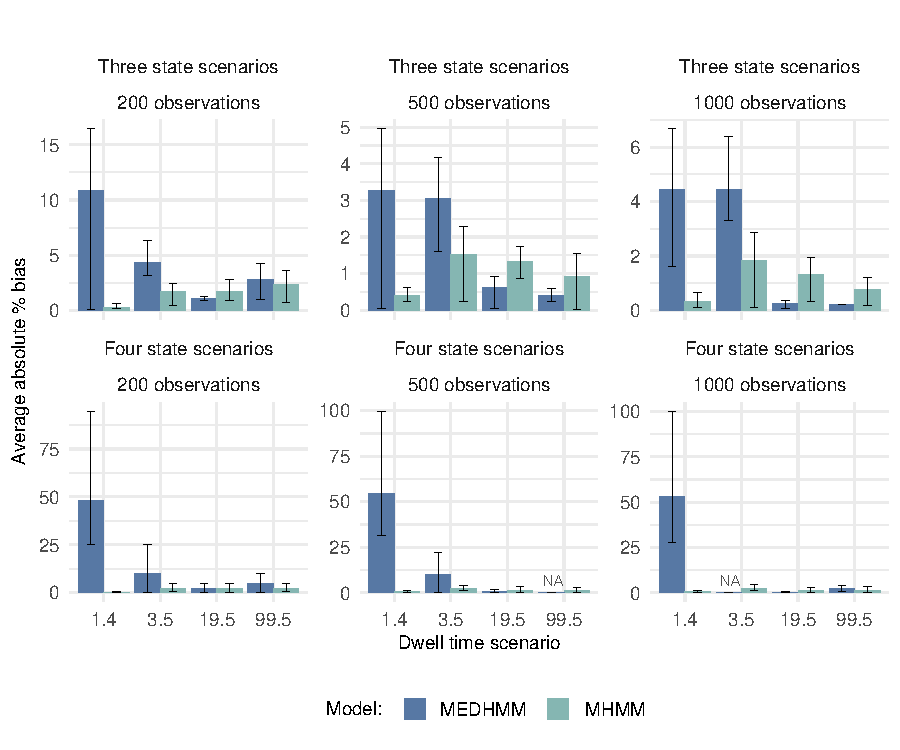
\includegraphics[width=0.8\textwidth]{graphics/transition_prob_biasv2.pdf}
    \flushleft
\footnotesize
\justifying
The bar plots represent the averaged over transition probabilities for the MHMM adjusted transition probabilities \% bias for each scenario (i.e. for the three-state scenario in MEDHMM we took the absolute \% bias of non-zero transition probability matrix (TPM) entries and calculated the mean of those values; for MHMM we adjusted the TPM such that the diagonal entries (self-transitions) were fixed to 0 and then proceeded as with the MEDHMM's TPM). The error bars represent the range of the absolute \% bias for the transition probability values within a given scenario and model. Each panel is the same state and observation scenario where the first row is the three-state scenario and the second plot is the four-state scenario. The y-axis indicates the dwell time scenario, and colours represent different models. 
    \label{trans_bias}
\end{figure}


\subsubsection{Dwell time distributions}
Note that the parameters of log-normal dwell time distribution were estimated and reported only by the MEDHMM. 

\emph{Bias}     Overall, the performance in bias for the log-means of the dwell time distribution improved with increasing assumed dwell times. The bias estimates did not depend on the varying number of states. The log-mean values were overestimated majorly for $d=1.4$ with bias equal form $324\%-686\%$ of the true value. The number of observations tended to reduce the absolute bias, but did not improve the estimates when $d=1.4$. Two scenarios with an observation length of $200$ and $d=99.5$ assumed were slightly underestimated, however, still did not exceed the cut-off value of acceptable bias. The relative bias for log-mean estimates was lower than $5\%$ in $47\%$ of scenarios. In terms of log-variances, the absolute bias estimates for MEDHMM were least significant for the scenarios with $d=19.5$. The model tend to overestimate the log-variances in general, and the bias was decreasing with the length of the observation sequence. The tendencies in the estimates were not dependent on the number of states estimated. Values of \% bias ranged from $-100\%$ to $142.9\%$. The bias was less than $5\%$ of the true value for $41\%$ of the log-variance parameters. The best results for log-variances were obtained for simulation scenarios with dwell times $d\in\{99.5, 19.5\}$ independently of the state and observations scenarios.

\emph{Precision}    Precision estimates (ESE) for the log-means were less than $0.001$ on the log scale and were ranging from $0.001$ to $0.6$ on the log scale for the log-variance components.

\emph{Coverage}     The coverage for the log-mean parameters reached an acceptable level of $92\%$ in $33\%$ of scenarios and was within the satisfactory range for scenarios with d=$19.5$ and d=$99.5$. The number of states and observations had no impact on the coverage scores for the parameters. Moreover, the coverage for the log-variance estimates was slightly better, since $46\%$ of the total cases had coverage above the acceptable threshold. The coverage rates of the log-variance were increasing with the assumed dwell time value, hence they were most satisfactory for $d=19.5$ and $d=99.5$ and no influence of the varying observation sequence or the number of states was recorded. 

In order to relate the MEDHMM dwell time estimates to MHMM the average absolute relative bias was calculated and shown in Figure \ref{exp_dwell_bias}. Note that we treated the median of the log-normal distribution and the expected value of the exponential distribution as the expected dwell time for the MEDHMM and MHMM accordingly. The comparison revealed that according to the average absolute bias, the MEDHMM expected state duration was further from the assumed truth for all scenarios with $d=1.4$. The average absolute relative bias within MEDHMM estimates tended to decrease with longer durations. On the other hand, the statistics calculated for the MHMM dwell time estimates became greater with longer dwell time scenarios and the values were more prominent for more complex four-state scenarios. 
\begin{figure}[h]
\caption{\\The average absolute relative bias for the expected dwell times } 
    \centering
    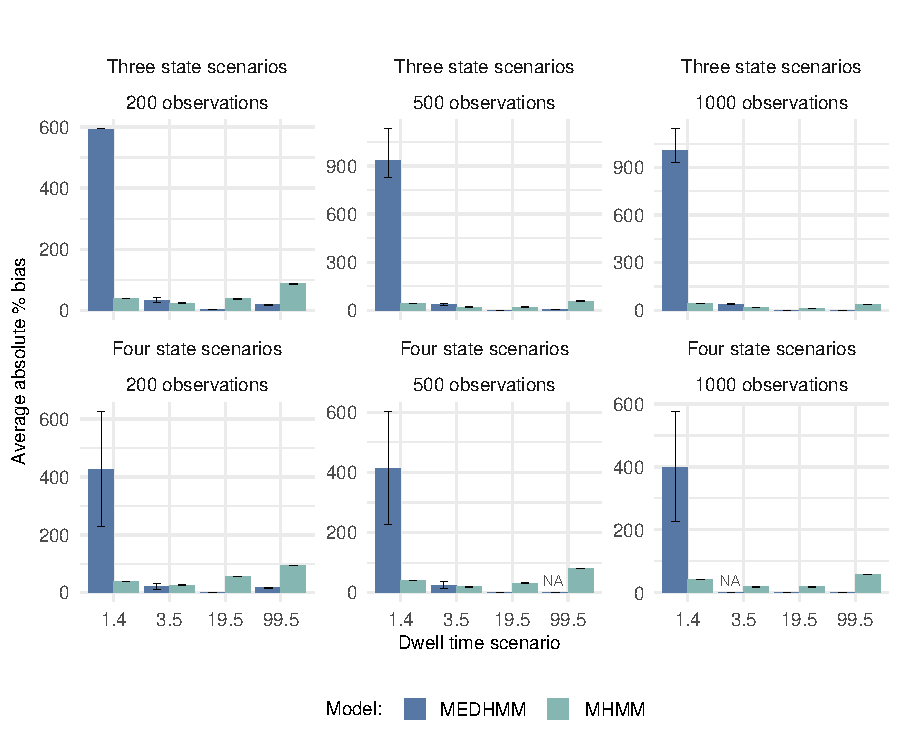
\includegraphics[width=0.8\textwidth]{graphics/expected_dwell_biasv2.pdf}
\flushleft
\footnotesize
\justifying
The bar plots represent the averaged over the state-specific expected dwell times \% bias for each scenario (i.e. for the three-state scenario in MEDHMM we took the absolute \% bias of the expected state durations for state 1, 2, and 3 and calculated the mean of those three values). The error bars represent the range of the absolute \% bias for the state-specific values within a given scenario and model. Each panel is the same state and observation scenario where the first row is the three-state scenario and the second plot is the four-state scenario. The y-axis indicates the dwell time scenario, and colours represent different models. 
\label{exp_dwell_bias}
\end{figure}

\subsubsection{State decoding derived measures}
The subject-specific state decoding was inspected in three ways: the proportion of states correctly decoded for each scenario visualized in Figure \ref{decoding_kappa}; the average number of switches in state decoding sequences in Figure \ref{state_switches} in Appendix B; and the average empirical duration of each state within given scenarios showed in Figure \ref{empiric_dwell} in Appendix B. In terms of decoding accuracy, the MHMM states were recovered in $99\%$ of scenarios. On the contrary, the MEDHMM recovered $81\%$ of the states' position. The state decoding for the MEDHMM failed for the shortest dwell times assumed. The MEDHMM did significantly worse for scenarios with a shorter duration of $d=1.4$ and $d=3.5$. However, for scenarios with dwell time $d=19.5$ and $d=99.5$ the Kappa statistic was greater for the MEDHMM when compared to the MHMM, but the differences were not larger than the $0.1\%$ change. The average number of switches for each scenario was recovered almost perfectly for the MHMM. The MEDHMM underestimated the average number of switches for the scenarios with $d=1.4$ and $d=3.5$. The estimated number of switches in MEDHMM tended to be closer to the switches count in simulated data with the increasing sequence length and number of states, especially for the $d=3.5$ scenario. In terms of the estimation of the state persistence according to the local decoding, the MHMM empirical dwell times were closer to in-sample dwell times for all simulation scenarios. The MEDHMM decoding showed overestimated state persistence when the shorter dwell time was assumed and was closest to the in-sample state duration for the scenario with the longest dwell time assumed d=99.5. 

\subsubsection{Additional Simulation scenario: Dwell time varying between hidden states}
 In general, the MEDHMM was able to recover varying dwell times across states. Log-means and log-variances were generally estimated within the satisfactory thresholds for bias and coverage, except for the log-means for the state with the shortest persistence, for which the value was slightly overestimated. The empirical standard deviations were smaller than $0.1$. The comparison of the expected state persistence showed that the MEDHMM was able to recover the expected durations, the MHMM underestimated the expected dwell time values and had difficulty estimating longer dwell times (see Table \ref{mix_table_exp_dwell}). Regarding the TPM parameter estimation, the MEDHMM did well in terms of bias and coverage with minor instabilities for two out of six parameters. On the other hand, the MHMM TPM estimates were not satisfactory, with only one probability recovered with satisfactory $\%bias$. In terms of the emission distribution means, the estimates derived by MEDHMM and MHMM were similar and had almost identical ESE. The Bias and coverage values for the mean parameters were acceptable for MHMM and mostly acceptable for MEDHMM (the first state means resulted in  $79.7\%$ coverage value). The variance components of the emission distribution were consistently overestimated by two models, and none of them reached acceptable coverage or bias. The ESE of the variances were larger for the MEDHMM and ranged from $1.4$-$12.4$ while for the MHMM they were between $1.8$ and $10.4$. In MHMM the self-transition probabilities were slightly underestimated however the self-transitions probabilities for the states with duration assumed to be $d=19.5$ and $d=99.5$ were close to the assumed proportions and only for these two TPM entries bias was less than 5\% of their expected true value. The TPM parameters for the MHMM had on average larger ESE when compared to MEDHMM and none of its parameters had satisfactory coverage. Regarding state decoding, the Kappa statistics were $99.7\%$ for the MEDHMM
and $99.9\%$ for MHMM. The average number of switches in-sample was $11$ and was recovered correctly by the MEDHMM while the MHMM average count of switches was $12$. The empirical dwell times derived from the local decoding mostly agreed with the in-sample estimates.  
All MAP estimates for the group-level parameters were summarised and are available for detailed inspection in Table \ref{mixed_sim} in Appendix D.

\begin{table}
\caption{The expected dwell times for the MEDHMM \& MHMM for varying between states dwell time scenario}
\centering
\begin{tabular}{cccccc} 
\toprule
 &  & \multicolumn{2}{c}{MEDHMM} & \multicolumn{2}{c}{MHMM} \\ 
\cmidrule{1-2}\cmidrule(lr){3-4}\cmidrule(lr){5-6}
State & Expected Dwell time & Median (ESE) & \% Bias & Median (ESE) & \% Bias \\ 
\midrule
1 & 3.5 & 3.94 (0.05) & 12.86 & 2.36 (0.16) & -32.08 \\
2 & 19.5 & 19.30 (0.06) & -0.67& 12.67 (1.14) & -34.99 \\
3 & 99.5 & 97.51 (0.05) & -2.21 & 69.30 (6.89) & -30.35 \\
\bottomrule
\label{mix_table_exp_dwell}
\end{tabular}
\end{table}


\begin{figure}[h]
\caption{\\The decoding accuracy (Kappa statistics) of all simulation scenarios and both models}
    \centering
    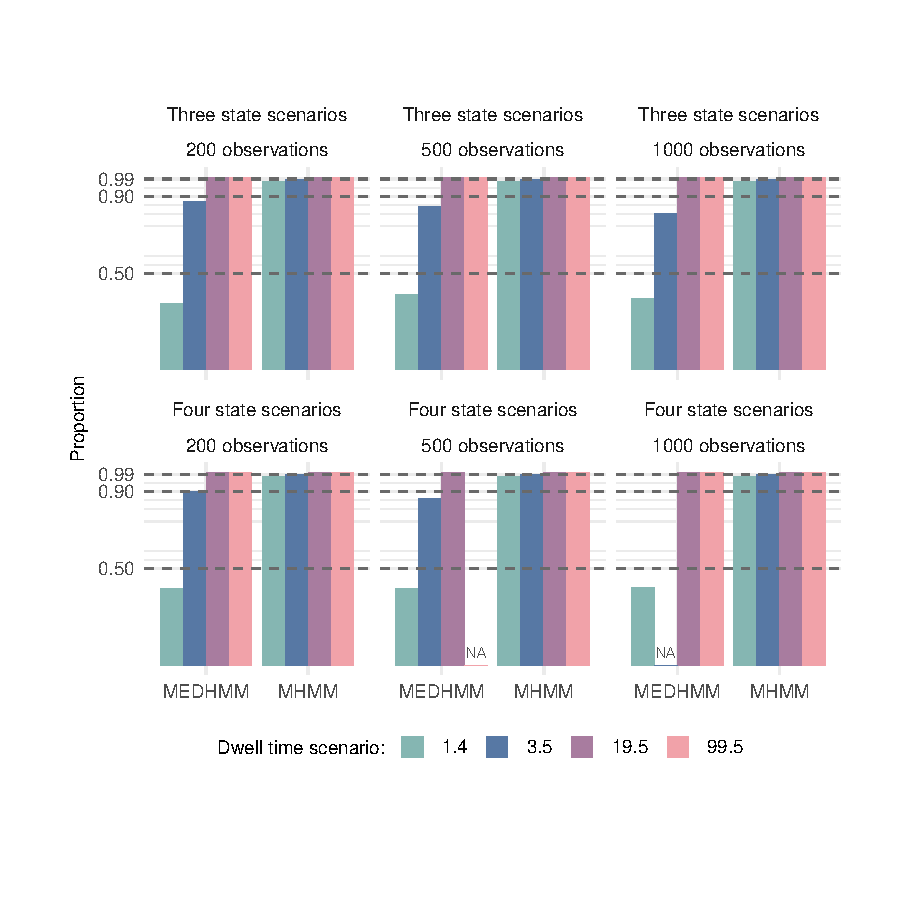
\includegraphics[width=0.8\textwidth]{graphics/state_decoding_simulation.pdf}
    \flushleft
    \footnotesize
    \justifying
    The bar plots show how Kappa statistics compare across varying simulation scenarios and models. Each panel is the same state and observation scenario where the first row is the three-state scenario and the second plot is the four-state scenario. The y-axis represents the models for which the statistics are calculated, and the colour is an indicator of the dwell time scenario.   
    \label{decoding_kappa}
\end{figure}
 \section{Empirical example of MEDHMM use: Bipolar disorder EMA data}
 Bipolar disorder (BD) is a psychiatric condition characterized by alternating episodes of mania and major depression \citep{Kukopulos_Reginaldi_Laddomada_Floris_Serra_Tondo_2008}. The illness consists of at least two mentioned discrete states (i.e. manic and depressive states) that interchange over time. The process is difficult to measure due to the lack of global indicators of the complex constructs of BD and the hidden character of its states. Instead, we can only record scores on the indicators of specific behaviours which are assumed to be the realization of underlying hidden states and use them to model hidden states' dynamics over time. A recent study showed that the \ac{mhmm} applied to the high-frequency data of BD patients is able to recover the dynamics of the psychiatric condition \citep{mildiner_moraga_bos_doornbos_bruggeman_van_2023} and model it as a system of four discrete phases (hidden states): manic, depressive, euthymic and mixed (i.e., high manic and depressive symptoms). In the current analysis, we will re-analyse the ecological momentary assessment (EMA) BD dataset that has been previously fitted with success to \ac{mhmm} in \cite{mildiner_moraga_bos_doornbos_bruggeman_van_2023}, and more broadly described in \citep{Bos_Krieke_2020, Bos_2022}. We hypothesized that the \ac{medhmm} would be preferable to the \ac{mhmm} in capturing the reflections of true BD state durations, leading to a more accurate estimation of the duration of the mood states, which would take a distribution that fits behavioural data better. In addition, since the \ac{medhmm} decouples the state durations and the off-diagonal transitions (transitions between two different states), the switching probabilities, which often take rather low values in the \ac{mhmm} applications, with \ac{medhmm} become larger, hence more significant, and robust. In this analysis we mainly focus on \ac{medhmm} results, however, the EMA dataset was also analysed with \ac{mhmm} to highlight the most prominent differences between the two models.

\subsection{Study overview}
 The detailed description of the BD study and items measured can be found in \cite{Bos_Krieke_2020}. Briefly, the study included twenty patients with bipolar disorder type I/II of $\geq 18$ years, under treatment at the time of the data collection, who reported at least two manic and/or depressive episodes in the previous year. The study was designed to assess the added value of long-term EMA in bipolar disorder treatment \citep{Bos_Krieke_2020} and to explore whether manic and depressive transitions can be anticipated with EMA data \citep{Bos_2022}. Participants completed five EMA questionnaires per day for at least four months, yielding over $9820$ assessments on $29$ EMA items. Every three hours, participants received a text message with a link to the EMA on their smartphone, which took 1–2 minutes to complete. All items were measured on $0-100$ visual analogue scales (ranging from ‘not at all’ to ‘very much’). Participants completed on average $18$ weeks of monitoring, except for two participants who completed $12$ weeks of monitoring as they were part of a pilot study. Weekly validated symptom questionnaires were also completed by each participant. The weekly questionnaires were: the 5-item Altman Self-Rating Mania Scale (ASRM; \citealp{Altman_Hedeker_Peterson_Davis_1997}), which measured manic symptoms on a scale of 0 to 4 (summing to 0-20), and the 16-item Quick Inventory for Depressive Symptomatology Self-Report (QIDS-SR; \citealp{Rush_2003}) used to assess depressive symptoms on a 0-3 scale (sum score ranges 0-48). Scores of 6 and above on both scales were indicators of potential (hypo)manic or depressive episodes \citep{Bernstein_Rush_Suppes_Kyotoku_Warden_2010}. Further demographic details of participants and the $29$ items EMA questionnaire aiming to measure momentary mood, symptoms, sleep, and activities can be found in \cite{Bos_Krieke_2020}. In the current study, we chose a subset of $12$ items following the \cite{mildiner_moraga_bos_doornbos_bruggeman_van_2023} choice. The $12$ EMA items were intended to measure manic states (“agitated”, “extremely well”, “irritated”, “full of ideas”, “racing thoughts”, “ability to focus/switch”) and depressive states (“down”, “tired”, “content”, “dreading the rest of the day”, “inadequate”, “worry”). On average, participants completed $76\%$ EMA assessments ($491$ assessments, SD=$137.8$) and $94-95\%$ of the QIDS and ASRM questionnaires. 
\subsection{Model Fitting}
Fitting models was done using the statistical software R (R Core Team, 2022) using developer versions of the \emph{mHMMbayes} and \emph{medHMM} packages. We trained both \ac{medhmm} and \ac{mhmm} with four hidden states. The choice of four state models was established based on the analysis performed in \cite{mildiner_moraga_bos_doornbos_bruggeman_van_2023} where the most appropriate number of states was four and was based on \ac{mhmm} trained on aggregated EMA data (\emph{depmixS4}; \citealp{Visser_Speekenbrink_2010}). The models were run with $2000$ iterations, a burn-in period of $1000$, and two chains. The priors for emission distributions were set to uninformative or weakly informative, and starting values for MCMC chains were estimation results from the expectation-maximization \ac{hmm} trained on pooled data. The convergence of the parameters of interest was inspected with trace plots and the multivariate potential scale reduction factor \citep{Brooks_Gelman_1998}. The fit was evaluated using posterior predictive checks similar to those reported by \cite{mildiner_moraga_bos_doornbos_bruggeman_van_2023}, and \cite{Schliehe_Diecks_Kappeler_Langrock_2012} where $500$ datasets were simulated using the models' outputs and the group-level and subject-level item mean have been compared with observed values to asset how well the models are able to recover the true in sample observed item means. Numerous comparisons were performed to compare the \ac{mhmm} and \ac{medhmm} performances and to link them to empirical data. We treated medians of the Bayesian posterior distributions of group- and patient-level parameters as point estimates and report them for, transition probabilities, emission distributions, and dwell time distributions (only for \ac{medhmm}). For the dwell time distribution to ease the interpretation of results, we multiplied the expected dwell times by 3 hours, as it was the in-between questionnaire period and all values were informed on the normal scale. In order to obtain the state sequence for each patient, local decoding has been applied \citep{Bishop_2013, Zucchini_MacDonald_2009}. The subject-level state decoding for both models and its temporal alignment with QIDS and ASRM questionnaires scores was inspected visually. Additionally, to access the persistence of states over time we calculated the expected dwell times, and the number of total switches between states based on locally decoded states. The emission distributions for all items were assumed normal. The dwell time distribution in \ac{medhmm} was assumed log-normal and any missing vales were omitted.
\subsection{Results}
\subsubsection*{Model convergence}
Both \ac{medhmm} and \ac{mhmm} did not encounter any convergence issues on the group-level parameters. The two chains converge to the common values with the multivariate potential scale reduction factor $R=\{1-1.2\}$ for the \ac{medhmm} and $R=1$ for all parameters of the \ac{mhmm} which was satisfactory.
Posterior predictive checks for the four-state \ac{medhmm} and \ac{medhmm} revealed a good fit for group-level and a mostly good fit for patient-level means of the twelve EMA items (MEDHMM: Figure \ref{ppc_out_mean_medhmm}; MHMM: Figure \ref{ppc_out_mean_mhmm} in Appendix C). The \ac{medhmm} performed slightly better on the group-level estimates and a bit worse in capturing the subject-level in sample values when compared to \ac{mhmm}.
\subsubsection*{State definitions: Emission Distribution}
The distribution of the group-level maximum a posteriori (MAP) estimates for emission distribution means and variances for \ac{medhmm} and \ac{mhmm} revealed a close alignment between  results (see Figure \ref{group_emission_emp} in Appendix C). The \ac{medhmm} recovered state compositions comparable to the ones found in \cite{mildiner_moraga_bos_doornbos_bruggeman_van_2023}. In Figure \ref{fig:emiss_ss} we illustrated  MAP estimates of EMA patient-specific emission distribution means for each state over the 12 EMA items. The four states recovered by the \ac{medhmm} were: euthymic, manic, mixed, and depressive. The euthymic state was characterised by low mean scores both on the manic state indicators (e.g., “irritated”, “agitated”) and the depressive state indicators (e.g, “down”, “worry”), with item “content” having the highest estimated emission out of all EMA items. The manic state exhibits mostly low estimated EMA means on depressive measures, while high on the mania-related items. The depressive state showed low estimated EMA means on manic measures and high scores on the depression-related EMA items. Lastly, the mixed state was composed of estimated EMA mean scores that had high values on both manic and depression-related items. The heterogeneity between the estimated patient-level means of the EMA items was noticeable and can be seen in the width of the mean estimates distributions in Figure \ref{fig:emiss_ss} (e.g. the estimate of the “agitated” EMA item mean in the mixed state was ${\mu}_{[agitated]mix.}=75.07$ (sd=$13.5$) for patient 4 and ${\mu}_{[agitated]mix.}=4.5$ (sd=$13.7$) for patient 6). 
\begin{figure}
\caption{\\ Distribution of the patient-specific mean estimates of 12 EMA items across MEDHMM mood states.}
 \centering
 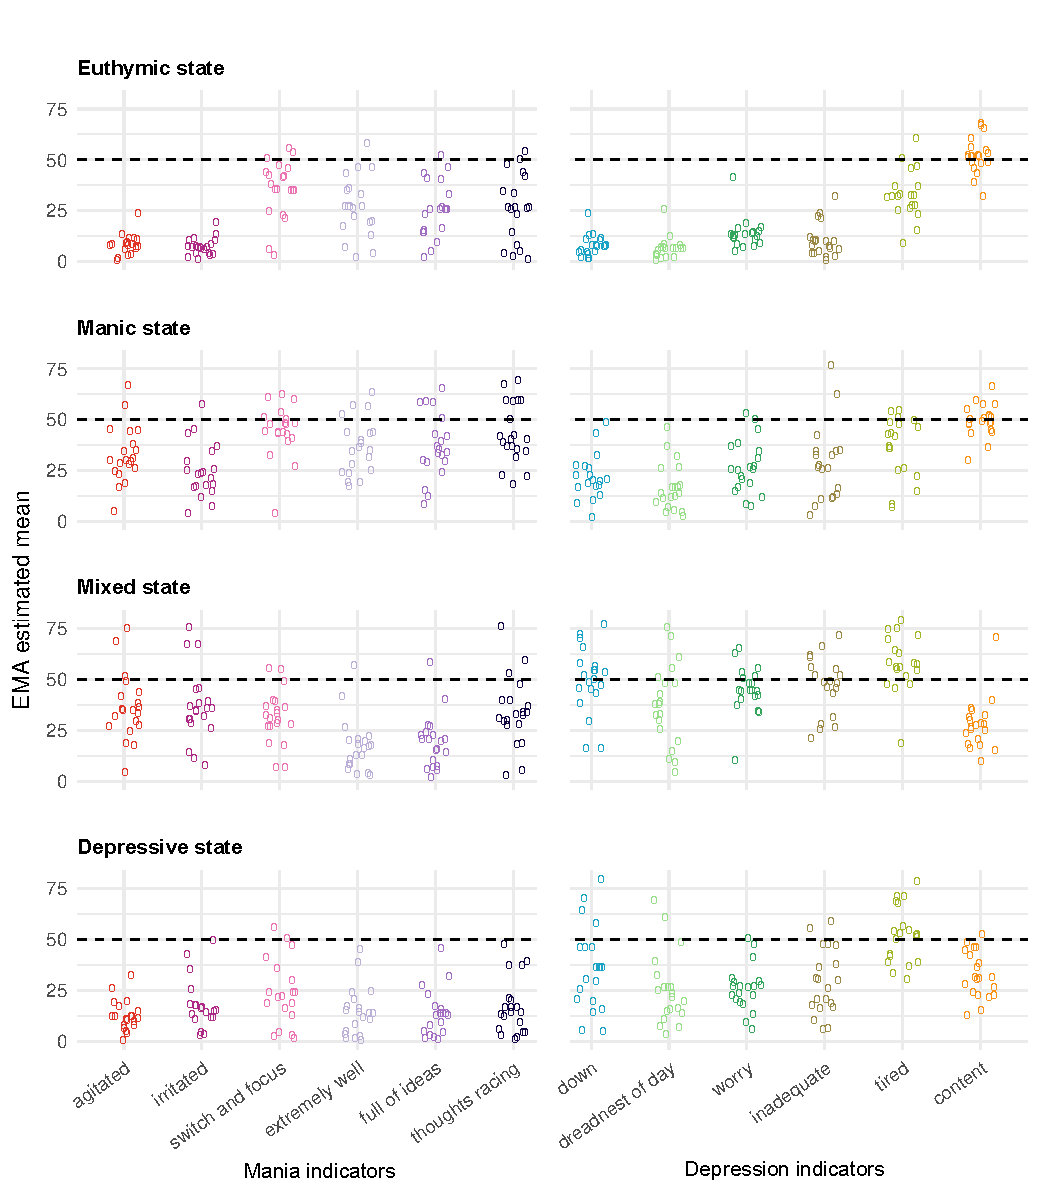
\includegraphics[width=0.8\textwidth]{graphics/ss_emiss.pdf}
  \flushleft
 \footnotesize
 \justifying
 The distribution of all patient-specific estimated emission distribution means for each EMA item is depicted in this figure. On the y-axis, we listed all the EMA items, with the first six being Mania indicators and the next six being Depression indicators. The value of the emission distribution mean is represented on the x-axis. To facilitate comparison, we marked the 50 score value with a dashed line because it is the centre of the possible value scale on all items.
 \label{fig:emiss_ss}
\end{figure}

\subsubsection*{Transitions between hidden Bipolar state: Transition distribution}
The group-level transition probability matrix (TPM) in Figure \ref{combined_ex}A visualizes the dynamics between bipolar states recovered by the \ac{medhmm}. The TPM revealed that the depressive state is the most probable to switch to when being in the euthymic state ($p_{({euth.\rightarrow depr.})}=0.63$ (sd$=0.11$)). When in the manic state, chances of switching to the euthymic ($p_{({man.\rightarrow euth.})}=0.36$ (sd$=0.11$)) and mixed ($p_{({man.\rightarrow mix.})}=0.39$ (sd$=0.15$)) were the largest. From the mixed state, the most probable switch was into the manic state ($p_{({mix.\rightarrow man.})}=0.5$ (sd$=0.15$)). Lastly, the switch to the euthymic state had the largest probability when being in the depressive state $p_{({depr.\rightarrow euth.})}=0.54$ (sd$=0.14$). Since in the \ac{medhmm}, the off-diagonal entries in TPM are redundant, we were also able to compare the outputs across rows (e.g. the group-level chance to switch to the manic state was most likely when the previous state was euthymic). Although the group-level TPM showed average estimated probabilities for the study group, patient-specific deviations to these parameters were present (e.g. the patient-level switching from euthymic to depressive state probability was in $\{0.12-0.94\}$ range). The examples of the patient-specific TPM are also shown in Figure \ref{combined_ex}C. We would like to acknowledge that the group-level TPM estimates of the MHMM were also assessed and revealed slightly different dynamics between mood states transitioning (see Figure \ref{emp_group_trans} in Appendix C for exact transition probability values for the transition matrix of MHMM). 

\begin{figure}[]
\caption{\\The MEDHMM results of group-level and subject-level transition probability matrices and the dwell-time distributions}
 \centering
 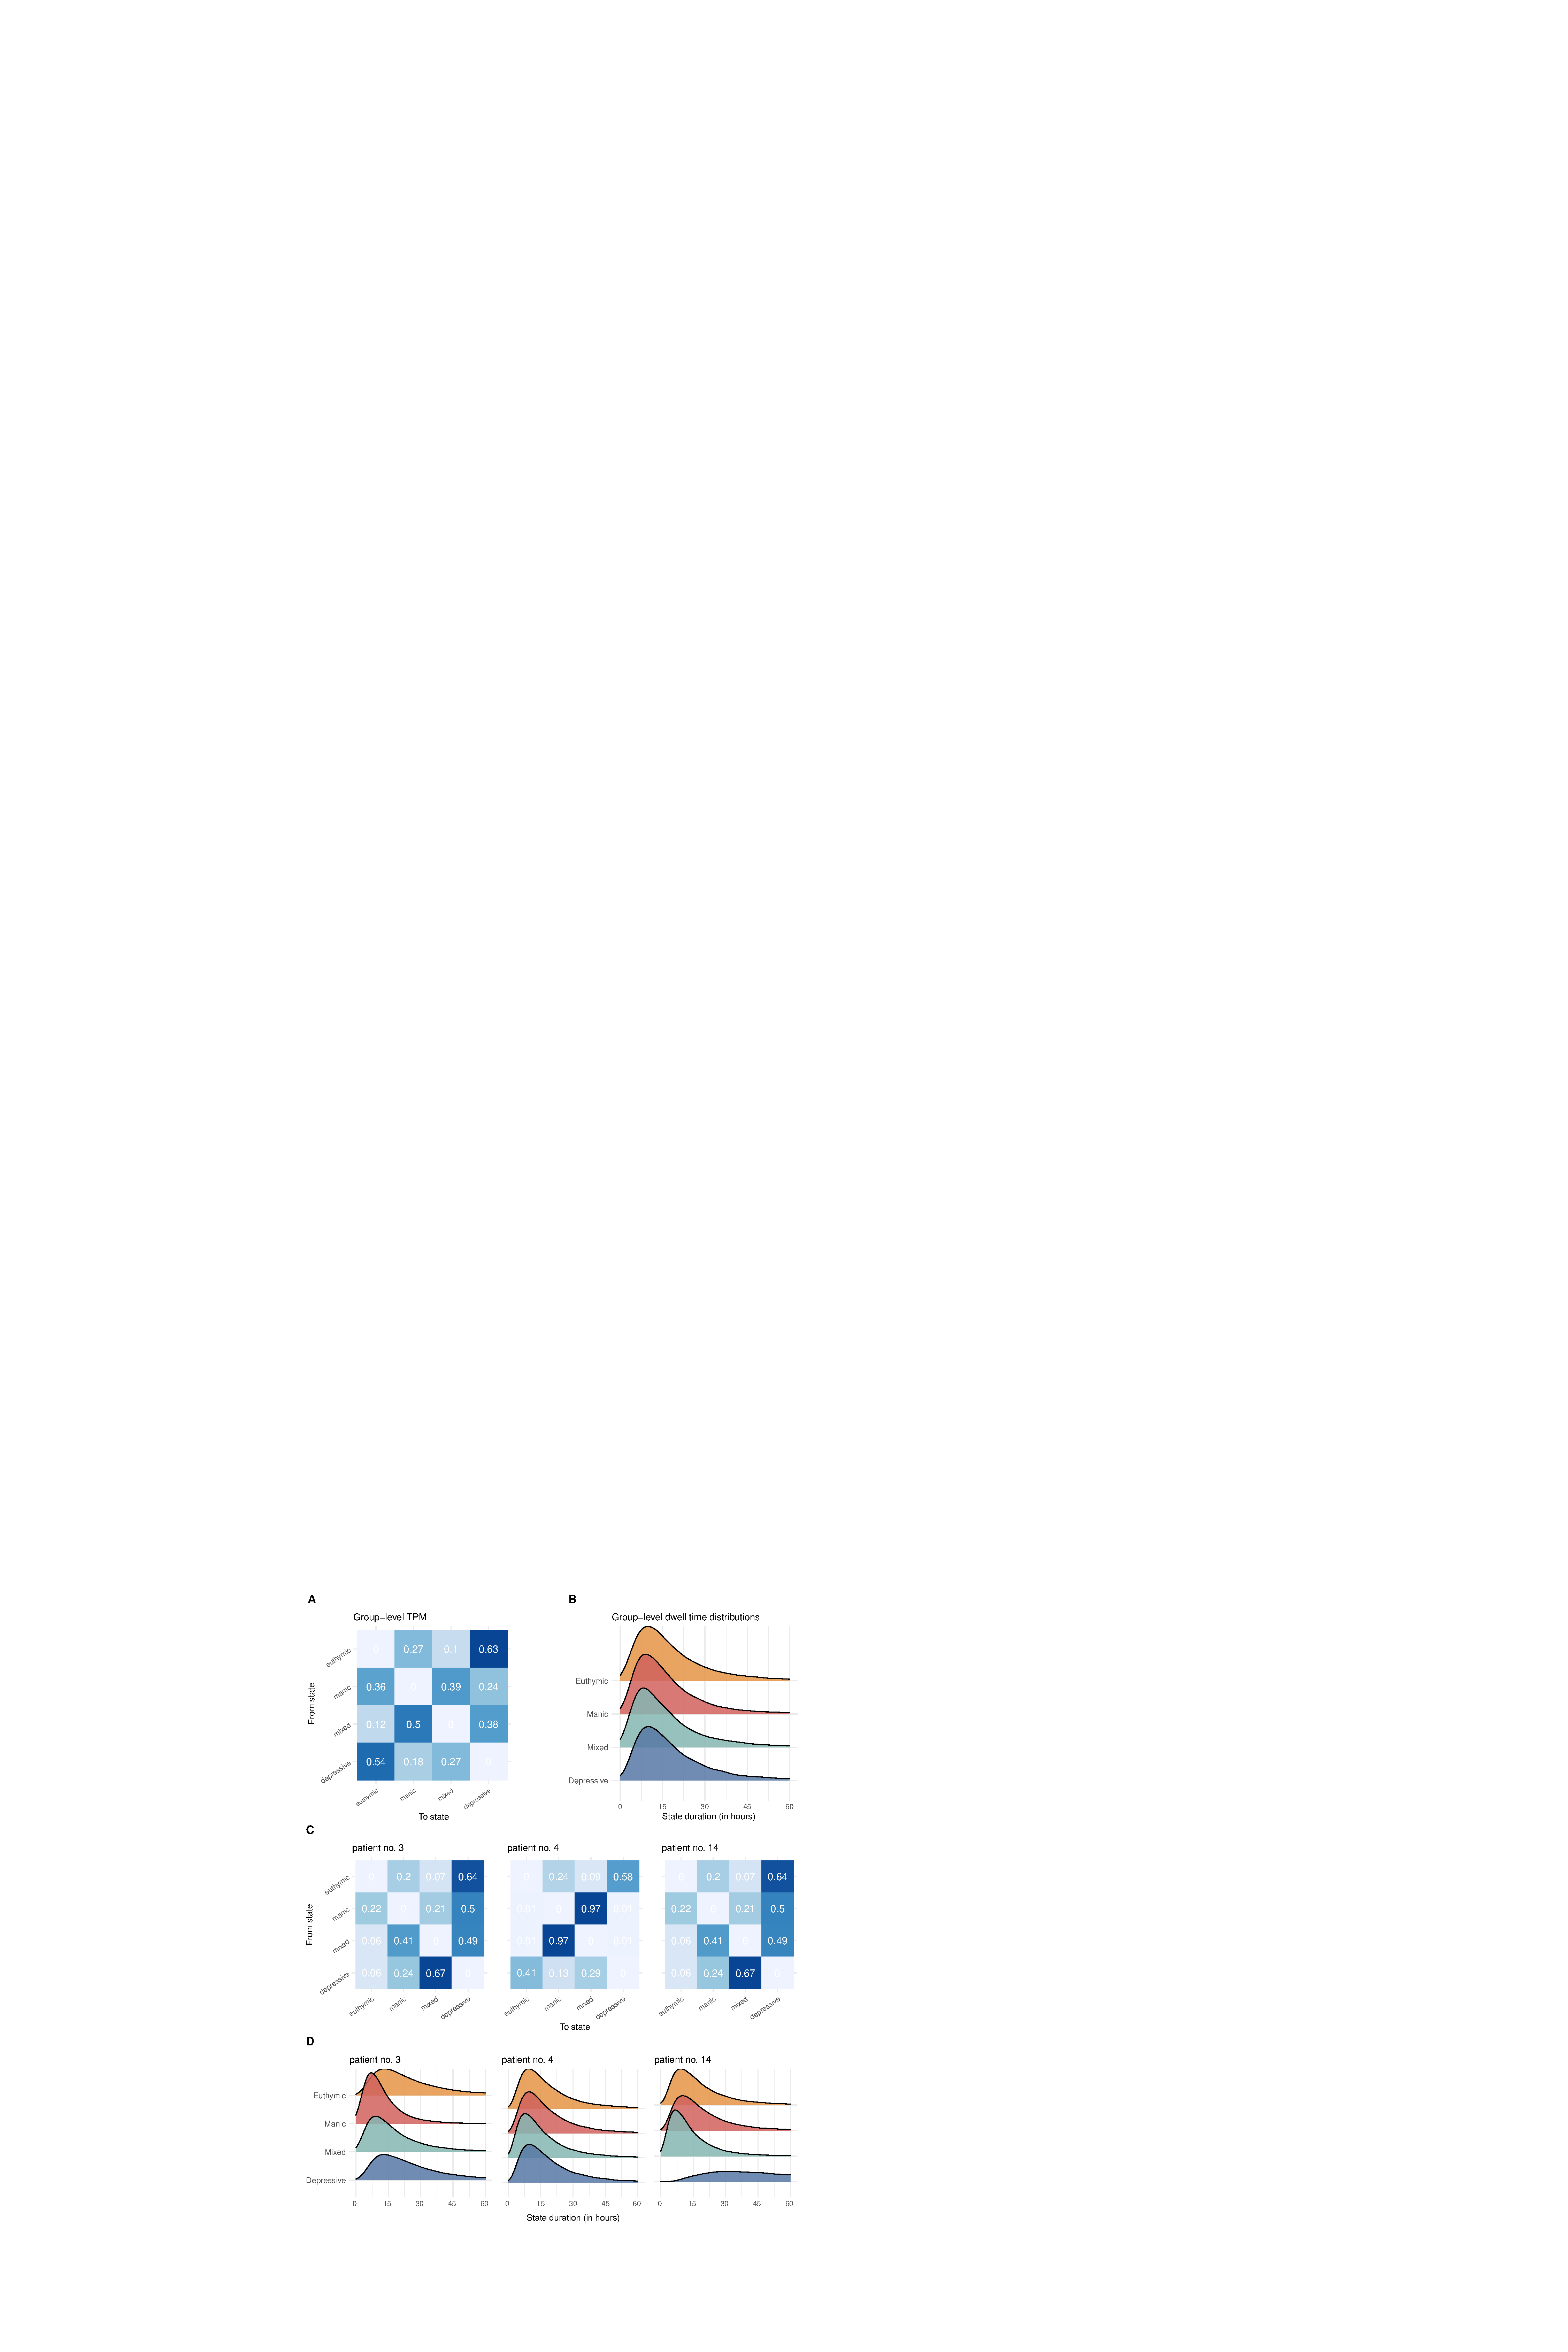
\includegraphics[width=0.75\textwidth]{graphics/empirical_example.pdf}
 \flushleft
 \footnotesize
 \justifying
Panel A shows the group-level transition probability matrix (note that the diagonal entries are equal to $0$); Panel B shows the group-level dwell time distribution for each Bipolar disorder (BD) mood state; Panel C shows the patient-specific (patient-level) transition probability matrices for three patients; Panel D shows the dwell time distributions derived for each BD mood state and are defined for three patients.
 \label{combined_ex}
\end{figure}

\subsubsection*{Bipolar states persistence: Dwell time distribution \& state switching count}
The dwell time distribution revealed that on the group level the expected (median) durations of bipolar states were: $15.10$h(sd$=5.38$h) for the depressive state, $14.61$h(sd$=5.09$h) for the euthymic state, $13.42$h(sd$=4.37$h) for the manic state, and $13.20$h(sd$=5.11$h) for the mixed state (see Figure \ref{fig:gamma_g1} for group-level distributions plotted). The model discovered large patient-specific deviations to the group-level mean, resulting in expected dwell times ranging: from $2.75$h for patient 11 to $13.32$h for patient 7 in the euthymic state; from $2.67$h for patient 17 to $11.25$h in the manic state; from $3.59$h for patient 14 to $6.69$h for patient 1 in the mixed state; and from $2.90$h for patient 7 to $17.90$h for patient 14 (see Table \ref{table_emp_switch} in the appendix for more detailed results). The standard deviations of the patient-specific dwell time distributions were different across subjects and states, with median standard deviations smaller in manic state sd=$\{2.64\text{h}-11.11\text{h}\}$ and more significant in depressive state sd=$\{3.10\text{h}-19.09\text{h}\}$. The count of switches between two different states within a patient observed sequence ranged between $0$ and $115$ switches per subject, and the counts added up to $0$ to $0.273$ proportion of total observations. We refer to Table \ref{table_emp_switch} for more details listed. 

\subsubsection*{Overall performance of MEDHMM when compared to MHMM}
In this part, we would like to draw the reader's attention to two most prominent differences between the MHMM and MEDHMM. 

Firstly, the inspection of overlap of weekly data and decoding derived for each subject for both models (see Figure 11 for example of 3 patients and Figure \ref{decoding_all} in Appendix C for the rest of patient-specific decodings). The MEDHMM resulted in fewer switches in comparison to the MHMM and established more comprehensive states. This result aligned with the outcomes of our simulation study, as the MEDHMM tends to smoothen state decoding more than MHMM. The MHMM decoding was sometimes more unclear with the rapid switches between states. There has been some mismatch in terms of recovered states, for example for patient 4 when the QIDS indicator started to rise from about the 250th observation the MEDHMM marked it as transition from Manic to Mixed state while the MHMM decoded it as transition from Manic to Depressive state through an unclear mixed/depressive mood segment (see middle panel of Figure 11A). Nevertheless, assessing the quality of the models' decoding would require the true sequence of true states for each patient, which is not possible. As an alternative, experts' knowledge in the form of interviews with patients and psychiatrists could be combined with the weekly symptom scores to shed light on this problem. 

Secondly, since the bipolar disorder states durations were assumed log-normal, by using the \ac{medhmm} we could visualise them and estimate for each patient separately. On the contrary, obtaining the direct dwell time distributions for \ac{mhmm} was not possible, and we could only use the self-transition probabilities to model dwell times with approximate exponential distribution. In Figure \ref{exp_ss_dwell} dwell time distributions derived from MHMM and MEDHMM were compared for three patients. We could see that the dwell time distribution of MHMM tended to overlap more than the distributions derived from MEDHMM. This might indicate that possibly some states last longer and the MEDHMM can distinguish them better. The results demonstrated that both models estimated the emission distribution means similarly (see \ref{group_emission_emp} in Appendix C). Given the outcomes from performed simulation study we found that whenever the emission distributions can be recognized, the dwell time distribution in MEDHMM introduced more information to the model resulting in more robust results. In addition, we know that the MEDHMM can distinguish between states when varying dwell times are present in data, which we experience in this dataset. For example, in Figure 12 we could see that for patient 14 the duration of the depressive state had the largest expected duration, which was also in line with the local decoding. That said, 
we believe that the MEDHMM performed better in modelling the dwell times. 

\subsubsection*{Conclusions}
We showed how the Multilevel Explicit Duration Hidden Markov Model can be applied to real empirical data. We modelled the bipolar disorder with four states by applying the MEDHMM that explicitly captured the distributions of mood states' durations. We confirmed the findings from our simulation study by showing that MEDHMM smoothens state decoding and can discover longer dwell times with log-normal distribution. All in all, in our opinion, the MEDHMM worked better in the dwell time estimations as it could capture longer dwell times with more accuracy. We believe that the gains in the accuracy of state decoding could be a promising outcome for practicians. By easing the diagnosis of early warning signals and minimizing the diagnosis to intervention time, this approach could help improve patient outcomes in future. 

\begin{figure}
\caption{\\Temporal alignment between mood states and weekly symptom scores}
    \centering
    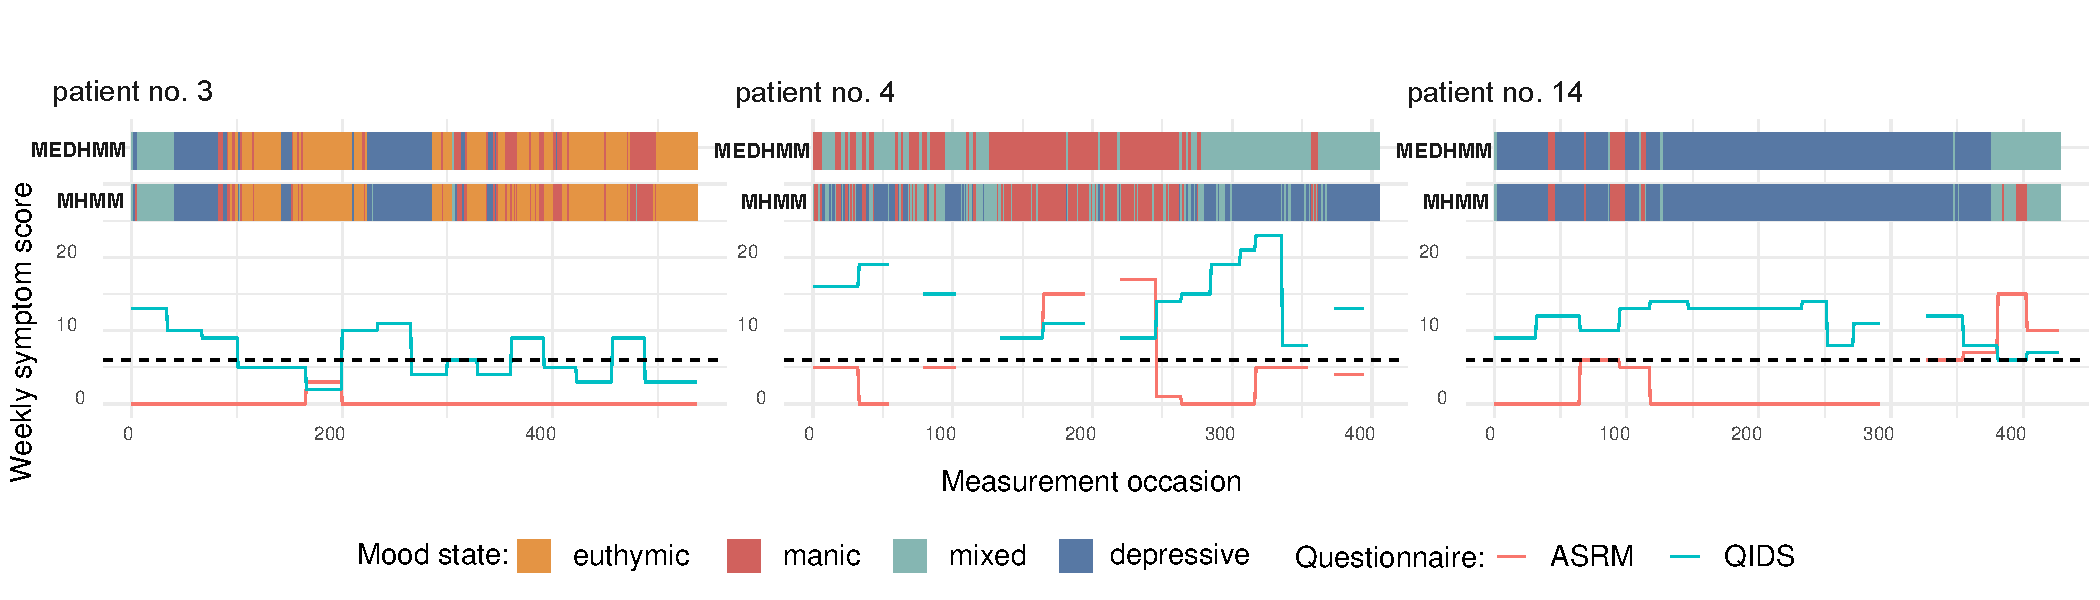
\includegraphics[width=1\linewidth]{graphics/decoding_14.pdf}
    \flushleft
    \footnotesize
    \justifying
    The figure shows local state decoding for the MEDHMM (upper decoding strip) and the MHMM (lower decoding script). The plots are presented for three BD patients to showcase the differences between state decoding. Below strip plots the alignment with the weekly symptom scores on the depressive behaviour indicator (QIDS) and manic behaviour indicator (ASRM).
    \label{quest_vs_decoding}
\end{figure}

\begin{figure}
\caption{\\Derived dwell time distributions for the MHMM and MEDHMM}
    \centering
    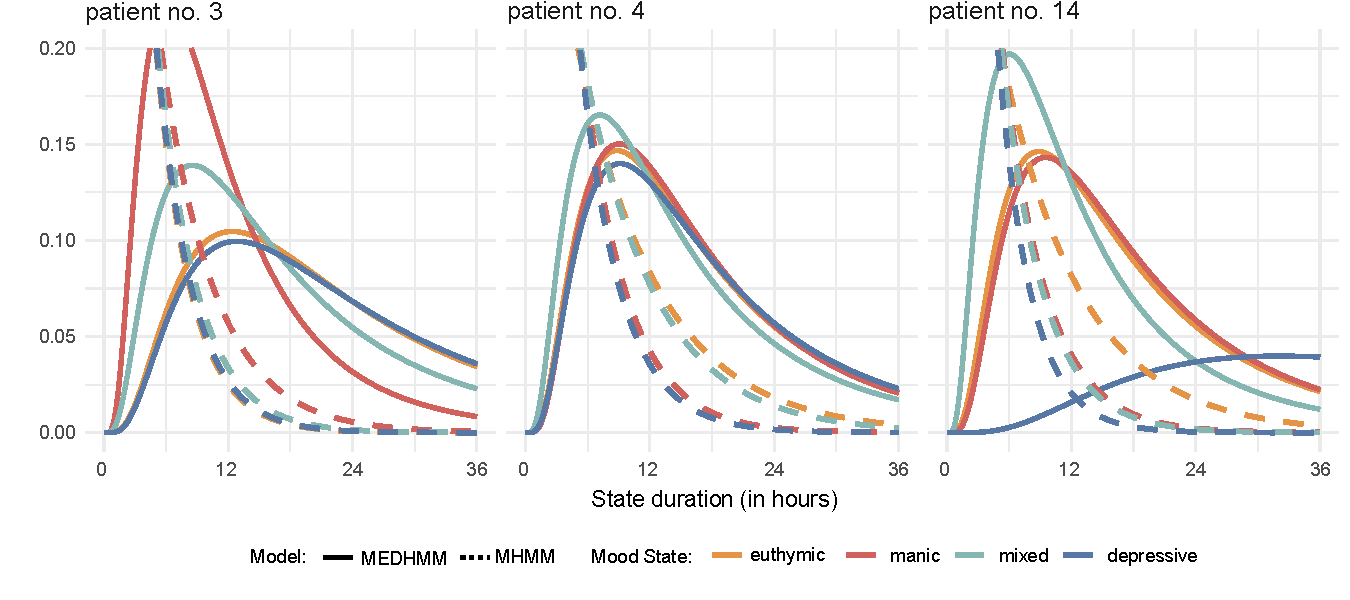
\includegraphics[width=1\linewidth]{graphics/expected_dwell_distr.pdf}
    \flushleft
    \footnotesize
    \justifying
    The plots show the comparison between dwell time distributions derived from MHMM and MEDHMM estimates for three patients from the BD study. The dashed lines represent state-specific exponential distributions that serve as an approximation of the geometric distribution that is assumed to model the dwell time in MHMM. The solid lines represent the dwell time distributions estimated by the MEDHMM that follow the log-normal distribution.
    \label{exp_ss_dwell}
\end{figure}


\section{Discussion}
In this thesis, we introduced the Multilevel Explicit Duration Hidden Markov model, a novel method to model hidden behavioural patterns with Intensive longitudinal data. We performed the Monte Carlo simulation study with varying levels of a number of states, state duration and observed sequence length in order to assess their effects on MEDHMM performance and compare it with the MHMM results under the same simulation scenarios. We explicitly aimed to answer the question if the more complex and computationally intensive MEDHMM can capture the true hidden state durations with greater accuracy than the MHMM and estimate the other model-specific parameters (i.e. group-level emission and gamma distribution parameters) with the same precision as the MHMM does. Bias, precision, and coverage were used to identify the performance of each model. Finally, to demonstrate the applicability of MEDHMM we applied the method to empirical Bipolar disorder data and show how it can be modelled to recover the bipolar disorder mood state dynamics for the intensive longitudinal study. 

\subsection{Main Findings}
The Monte Carlo study revealed that the MEDHMM can outperform the MHMM in dwell time estimation, as well as, in the estimation of other state-specific group-level parameters when state durations are greater or equal to $19.5$. On the other hand, the MEDHMM failed to recover the true emission distribution means for a shorter dwell time of $1.4$ and for some scenarios with state durations equal to $3.5$. Further, results showed the MEDHMM performed slightly better than the MHMM in state decoding accuracy for the longer state durations. The results from the additional scenario, with varying across states dwell times, showed that the MEDHMM performed well in the estimation of group-level parameters. This suggested that the MEDHMM is able to distinguish between states more effectively when state durations are not equal, which is in line with \cite{Ruiz_Suarez_2022}. We demonstrated that the MHMM could perform well in modelling the state-specific emission distributions overall. In addition, the MHMM was able to capture the shorter durations of states better. We also saw that the MHMM overestimated the self-transition probabilities and underestimated the switching between two different states probabilities. This result was in line with the existing research on Multilevel Hidden Markov models, as \cite{McClintock_2021} and \cite{jonsen2016joint} point out that estimating transition parameters which are closer to the parameters' space boundaries (i.e., 0 and 1) are more challenging to establish for MHMM. Nevertheless, the results from the adjusted transition matrix without diagonal entries confirmed that the MHMM can recover the true transition probabilities assumed by the simulation study well, however still not as good as the MEDHMM when longer dwell times are assumed. 

Having the main findings listed, we would like to further describe how each simulation factor influenced the estimates of the current study. 

We showed that with increasing dwell time, the performance of MEDHMM of estimation of all parameters improved significantly and results were more accurate than for MHMM. Our findings were in line with \cite{Ruiz_Suarez_2022} who investigated the effect of varying dwell time for single-level EDHMM and HMM. Similar to them, we found that the model decoding accuracy of MEDHMM exceeds the accuracy of the MHMM for longer states. Also in line with the results in \cite{Ruiz_Suarez_2022}, we saw that the dwell time estimation is more accurate when the assumed dwell time is long or differs within states. However, our conclusion is limited to one additional scenario with different state duration we investigated and further durations that are needed to establish it. For the dwell time distributions, we saw that for scenarios with assumed $1.4$ state duration, the MEDHMM was not able to estimate the dwell time means parameters accurately. The reason for that is the low density around $0$ values for the log-normal distribution, which make the distributions not suitable for modelling short time durations and cannot account for the inflated amount of state durations of $1$ (\citealp{hadjamar2022bayesian}). 

With the increase in the number of observations, parameter estimates from the MHMM exhibit marginally decreasing bias and increased precision and coverage (e.g., \citealp{McClintock_2021}). In terms of the MEDHMM parameter estimation, we observed the same tendencies. The results were expected as with the increasing amount of information the models had more power to estimate parameters of posterior distribution more accurately.  

The effect of increasing number of states was not as prominent as the effects for varying state durations and observation sequence lengths. On average, the coverage of group-level parameters was larger and the bias was smaller for the $3$ state model in comparison to the $4$ state scenarios for both methods. According to \cite{LUATI2021107183} for a single-level EDHMM the accuracy of the decoding should decrease with the number of states. Our results did not agree as for the MEDHMM we recorded improvements in decoding accuracy when comparing $3$ and $4$ state scenarios. 

\subsection{Limitations}
Nonetheless, the founding of our research must be interpreted with caution and some limitations should be borne in mind.
Firstly, the simulation was designed in such a way that the dwell times were equal over states. That way we were able to capture the effect of increasing dwell time, however, the effect of varying dwell times that may often accrue in real data was not assessed. The work of \cite{Ruiz_Suarez_2022} showed that the single-level EDHMM is able to capture scenarios with varying dwell times well, we could confirm the finding only through the extent of our additional simulation scenario where we assumed  different dwell times across 3 proposed states and 500 observations per subject. Nevertheless, more extensive research would have to be implemented in order to make the result valid for a wider range of possible scenarios. 

Secondly, we used the log-normal distribution to model the state durations in MEDHMM which appeared not an appropriate choice for modelling durations that were short and close to $1$. Multiple studies of single-level EDHMMs proposed different dwell time distributions. For example, \cite{hadjamar2022bayesian,dewar_inference_2012,LUATI2021107183} proposed Poisson and shifted Poisson distribution, \cite{hadjamar2022bayesian,POHLE2022107479} proposed Negative binomial distribution and \cite{Nagaraja_1996} used inverse gamma distribution. We would expect some of them to be a better fit for shorter durations or generalize well for a wider spectrum of state durations. That said, further research is required in order to implement and evaluated different distribution types for modelling intensive longitudinal data with the MEDHMM. 

Thirdly, our research showed that the simulated data were easy to solve for the MHMM as the simulation considered the state-dependent emission distributions to exhibit a low overlap, which was in line with \cite{McClintock_2021}. As a result, we could not access the effect of noisy or more imperfect states definitions. Generally, Hidden Markov models are known to perform poorly when the state-dependent distributions highly overlap (e.g. \cite{jonsen2016joint,Beyer_Morales_Murray_Fortin_2013}). The study of \cite{Ruiz_Suarez_2022} showed that the EDHMM can outperform the HMM when the overlap between state emission distributions is high, as the information about state durations allows the EDHMM to differentiate between states.  Because the HMM (and MHMM) rely solely on emission distributions to differentiate between states, it is expected that this model will fail when the emission distributions overlap. Those results, if applicable for MEDHMM, could introduce promising added value of recovering the emission distributions for noisy or highly overlapping data, as it is expected to experience not-so-well-defined states in empirical applications.

Lastly, we would like to point out that the execution models took considerably more time for the MEDHMM (23 hours on average) than the MEDHMM (2 hours on average). The significant difference between computational times was expected, as the structure of the forward-backwards algorithm for MEDHMM requires an additional step of calculating the most probable state duration for each value in range $1:d_{max}$. In MHMM, this calculation is not present, making the model more time efficient. Some studies of single-level EDHMM proposed different techniques to optimize the process, however, more investigation is required to improve the time of estimation. 

 

\subsection{Recommendations}
In this part, we summarized some recommendations for researchers planning to analyse ILD using MEDHMM or MHMM. \\\\
\emph{When focusing on emissions?}\\
If the researcher's focus is on obtaining the distributions of the observable data within established hidden states (emission distribution), the MHMM serves well independently of the duration of each state, the total number of states and the observation length. For longer state durations (i.e. d$\in{19.5, 99.5}$) the emission distribution parameters are closer to the truth, and we can expect that even for the observation length of 200 the variances perform better in terms of the bias than the MHMM.  \\ \\
\emph{When focusing on dwell times?}\\
If one wishes to recover the expected dwell times, there are a few options. When certain about the expected state persistence being longer than 20-time occasions, one should consider the use of the MEDHMM over the MHMM. In addition, we would always advise incorporating prior information about the dwell time distribution, which as shown in \cite{hadjamar2022bayesian} can lead to greater accuracy in dwell time parameters' estimation. Priors for expected state durations are not present in HMM. If the researcher is not sure about the expected dwell times, the less computationally intensive MHMM should be implemented as it gives the reader some guidelines about the expected state duration or at least the values can be used to establish more and less frequent states. \\ \\
\emph{When focusing on transition probabilities?}\\
We showed that MEDHMM recognizes the transition probabilities well, except in the scenario with the 1.4 dwell time. However, if one wishes to focus on the transitions between latent states, the adjusted transition probability matrix (excluding self-transitions) derived from MHMM results serves well in terms of recognizing the correct probabilities when the probabilities of the switch are equal. The computational time, especially for the longer observation sequences, might escalate quickly for the MEDHMM. 
We want to mention that our study did not test scenarios with unequal transition probabilities, hence the advice should be taken in light of the limitation. \\\\
\emph{When focusing on decoding?}\\ 
If one expects the dwell time to be longer than $3.5$ in light of our study, the decoding will be slightly more accurate for the MEDHMM. That said, if we would like to only focus on the decoding performance, the MHMM should be used as it can recognize both the state decoding with an overall accuracy of $\kappa>0.97$. The cautious however needs to be taken as in the current study we only inspected well-separated emission distributions and that's why the MHMM algorithm could use the estimates to correctly assess states. When the emission distributions would overlap a lot, the accuracy of the MEDHMM is expected to increase, as shown in \cite{Ruiz_Suarez_2022}. 



\section{Conclusions}
Our findings suggest that the novel Multilevel Explicit Duration Hidden Markov model is a promising approach to accurately model durations of latent states. The simulation study showed that the MEDHMM with log-normal dwell time distribution is able to capture longer state durations ($\geq19.5$) with greater accuracy than the Multilevel Hidden Markov model. Moreover, the MEDHMM outperformed the MHMM in estimating other model-specific group-level parameters (e.g. emission means, and transition probabilities) when longer dwell times were assumed. Nevertheless, the proposed MEDHMM was shown to be not well suited for the estimation of shorter dwell times ($\leq3.5$) %as it consistently underestimated the values of expected state durations 
and struggled to capture the means of emission distribution correctly contrary to MHMM that performed well for these scenarios. The results also confirmed that the performance of the MEDHMM can be improved when the dwell time is different across states. Despite some limitations, this study can serve as a starting point for future investigation of Multilevel Explicit Duration Hidden Markov models. We believe that further research and refinement of this model could lead to better estimation results, as well as new insights and advancements in a variety of fields, including psychology and behavioural sciences.
\section*{Ethical Approval}
The study was approved by the Ethical Review Board of the Faculty of Social and Behavioural Sciences of Utrecht University (ref.no 22-1845 and 22-1844).
\section*{Data availability statement}
The data that support the findings for the bipolar disorder example are available from upon reasonable request to University Medical Center Groningen (UMCG).
\section*{Supplementary materials}
All code used for the analysis has been stored in GitHub repository and is open to access via the link: \url{https://github.com/a-dacko/MEDHMM\_vs\_MHMM}.
\section*{Funding}
This work made use of the Dutch national e-infrastructure Snellius with the support of the
SURF Cooperative using grant no. EINF-2570, which is (partly) financed by the Dutch
Research Council (NWO).

\printacronyms[name=Abbreviations]

\bibliographystyle{apacite}
\bibliography{citations/references}

\section{Appendices}
\appendix
\section{Data simulation: Supplementary materials}
\begin{figure}[h]
\caption{\\Emission distributions for each of the state scenarios.} \centering
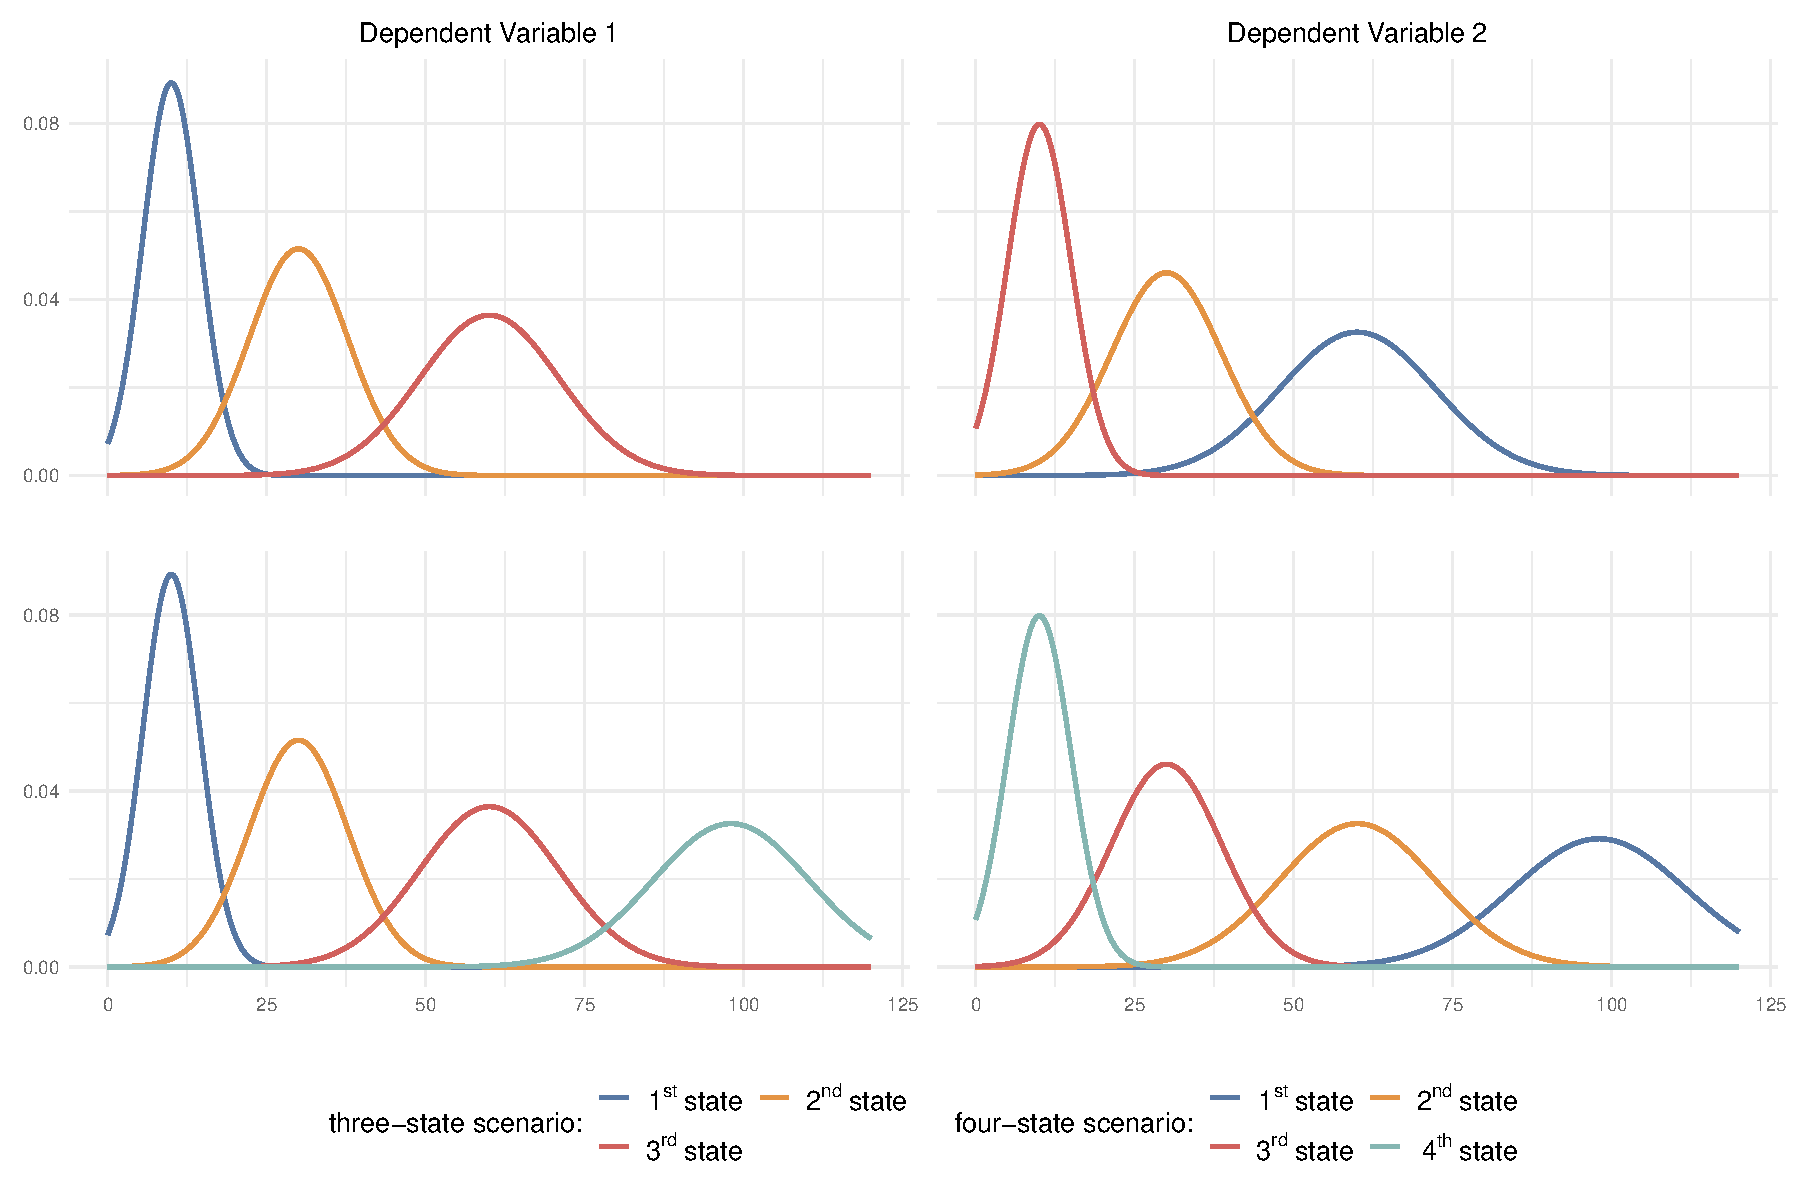
\includegraphics[width=0.75\textwidth]{graphics/emiss_dist_plot.pdf}
\label{em_ds}
\end{figure}

\begin{figure}[h]
\caption{\\Assumed dwell time distributions}
\centering
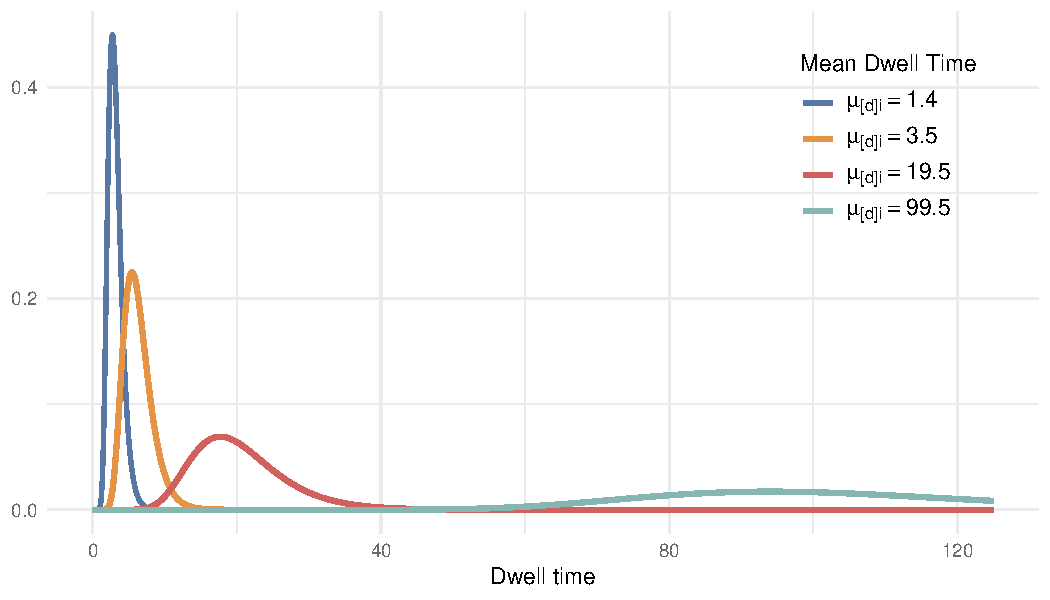
\includegraphics[width=0.7\textwidth]{graphics/lognorm_dist_plot.pdf}
\flushleft
\footnotesize
Three dwell time distributions used in the simulation study, with median dwell times ${d\in\{1.4,3.5,19.5,99.5\}}$\\
\label{log_ds}
\end{figure}

\begin{table}[h]
\caption{Emission distribution priors used in simulation study}
\centering
\resizebox{0.75\linewidth}{!}{
\begin{tabular}{p{0.15\textwidth}p{0.35\textwidth}p{0.3\textwidth}}

\toprule
\multicolumn{1}{c}{\textbf{Parameter}} & \multicolumn{1}{c}{\textbf{Description}} & \multicolumn{1}{c}{\textbf{Value}} \\
\midrule
\multicolumn{1}{c}{$\mu_{10},\mu_{20}$} & The hypothesized mean values of the Normal emission distributions in each of the states for each dependent variable.& \multicolumn{1}{c}{$\{10,30,60,98\}$, $\{98,60,30,10\}$} \\
\multicolumn{1}{c}{$\kappa_0$} & The number of hypothetical prior subjects on which the means $\mu_{10}$ and $\mu_{20}$ are based on. & \multicolumn{1}{c}{$1$}\\
\multicolumn{1}{c}{$u$} & The degree of freedom of the Inverse Gamma hyper-prior distribution connected to the emission distribution means. & \multicolumn{1}{c}{$1$} \\
\multicolumn{1}{c}{$V$} & The hypothesized variances between the subject-level means of the Inverse Gamma hyper-prior distribution connected to the emission distribution means. & \multicolumn{1}{c}{$100$}  \\
\multicolumn{1}{c}{$\alpha_0$} & The shape parameter value of the Inverse Gamma hyper-prior on each of fixed variances of the Normal emission distributions & \multicolumn{1}{c}{$0.001$}\\
\multicolumn{1}{c}{$\beta_0$} & The scale parameter values of the Inverse Gamma hyper-prior on each of fixed variances of the Normal emission distributions & \multicolumn{1}{c}{$0.001$} \\
\bottomrule
\label{Ap_emiss_hp}
\end{tabular}}
\end{table}

\begin{table}[h]
\caption{Dwell time distribution priors used in simulation study}
\centering
\resizebox{0.75\linewidth}{!}{
\begin{tabular}{p{0.15\textwidth}p{0.35\textwidth}p{0.3\textwidth}}
\toprule
\multicolumn{1}{c}{\textbf{Parameter}} & \multicolumn{1}{c}{\textbf{Description}} & \multicolumn{1}{c}{\textbf{Value}} \\
\midrule
\multicolumn{1}{c}{$\mu_{[d]0}$} & The hypothesized mean values of the log-Normal dwell distribution for each of the states in the logarithmic scale. & \multicolumn{1}{c}{$\{1.4, 3.5,19.5,99.5\}$} \\
\multicolumn{1}{c}{$s^2_0$} & The hypothesized variances between the between-subject level means of the Inverse Gamma hyper-prior distribution connected to the dwell distribution log-means. & \multicolumn{1}{c}{$10$} \\
\multicolumn{1}{c}{$\alpha_{\sigma^20}$} & The shape values of the Inverse Gamma hyper-prior on each of fixed variances of the log-Normal dwell distribution.
& \multicolumn{1}{c}{$0.01$} \\
\multicolumn{1}{c}{$\beta_{\sigma^20}$} & The scale values of the Inverse Gamma hyper-prior on each of fixed variances of the log-Normal dwell distribution. & \multicolumn{1}{c}{$0.01$} \\
\multicolumn{1}{c}{$\alpha_{\tau^20}$} & The shape values of the Inverse Gamma hyper-prior on each of the between-subject variances of the Normal prior on the dwell distribution. & \multicolumn{1}{c}{$0.01$}\\
\multicolumn{1}{c}{$\beta_{\tau^20}$} & The scale values of the Inverse Gamma hyper-prior on each of the between-subject variances of the Normal prior on the dwell distribution. & \multicolumn{1}{c}{$0.01$}\\
\bottomrule 
\label{Ap_dwell_hp}
\end{tabular}}
\end{table}

% \subsubsection{Empirical Example}


\section{Simulation Study: Selected results}
\begin{figure}[h]
\caption{Emission distribution: Precision}
    \centering
    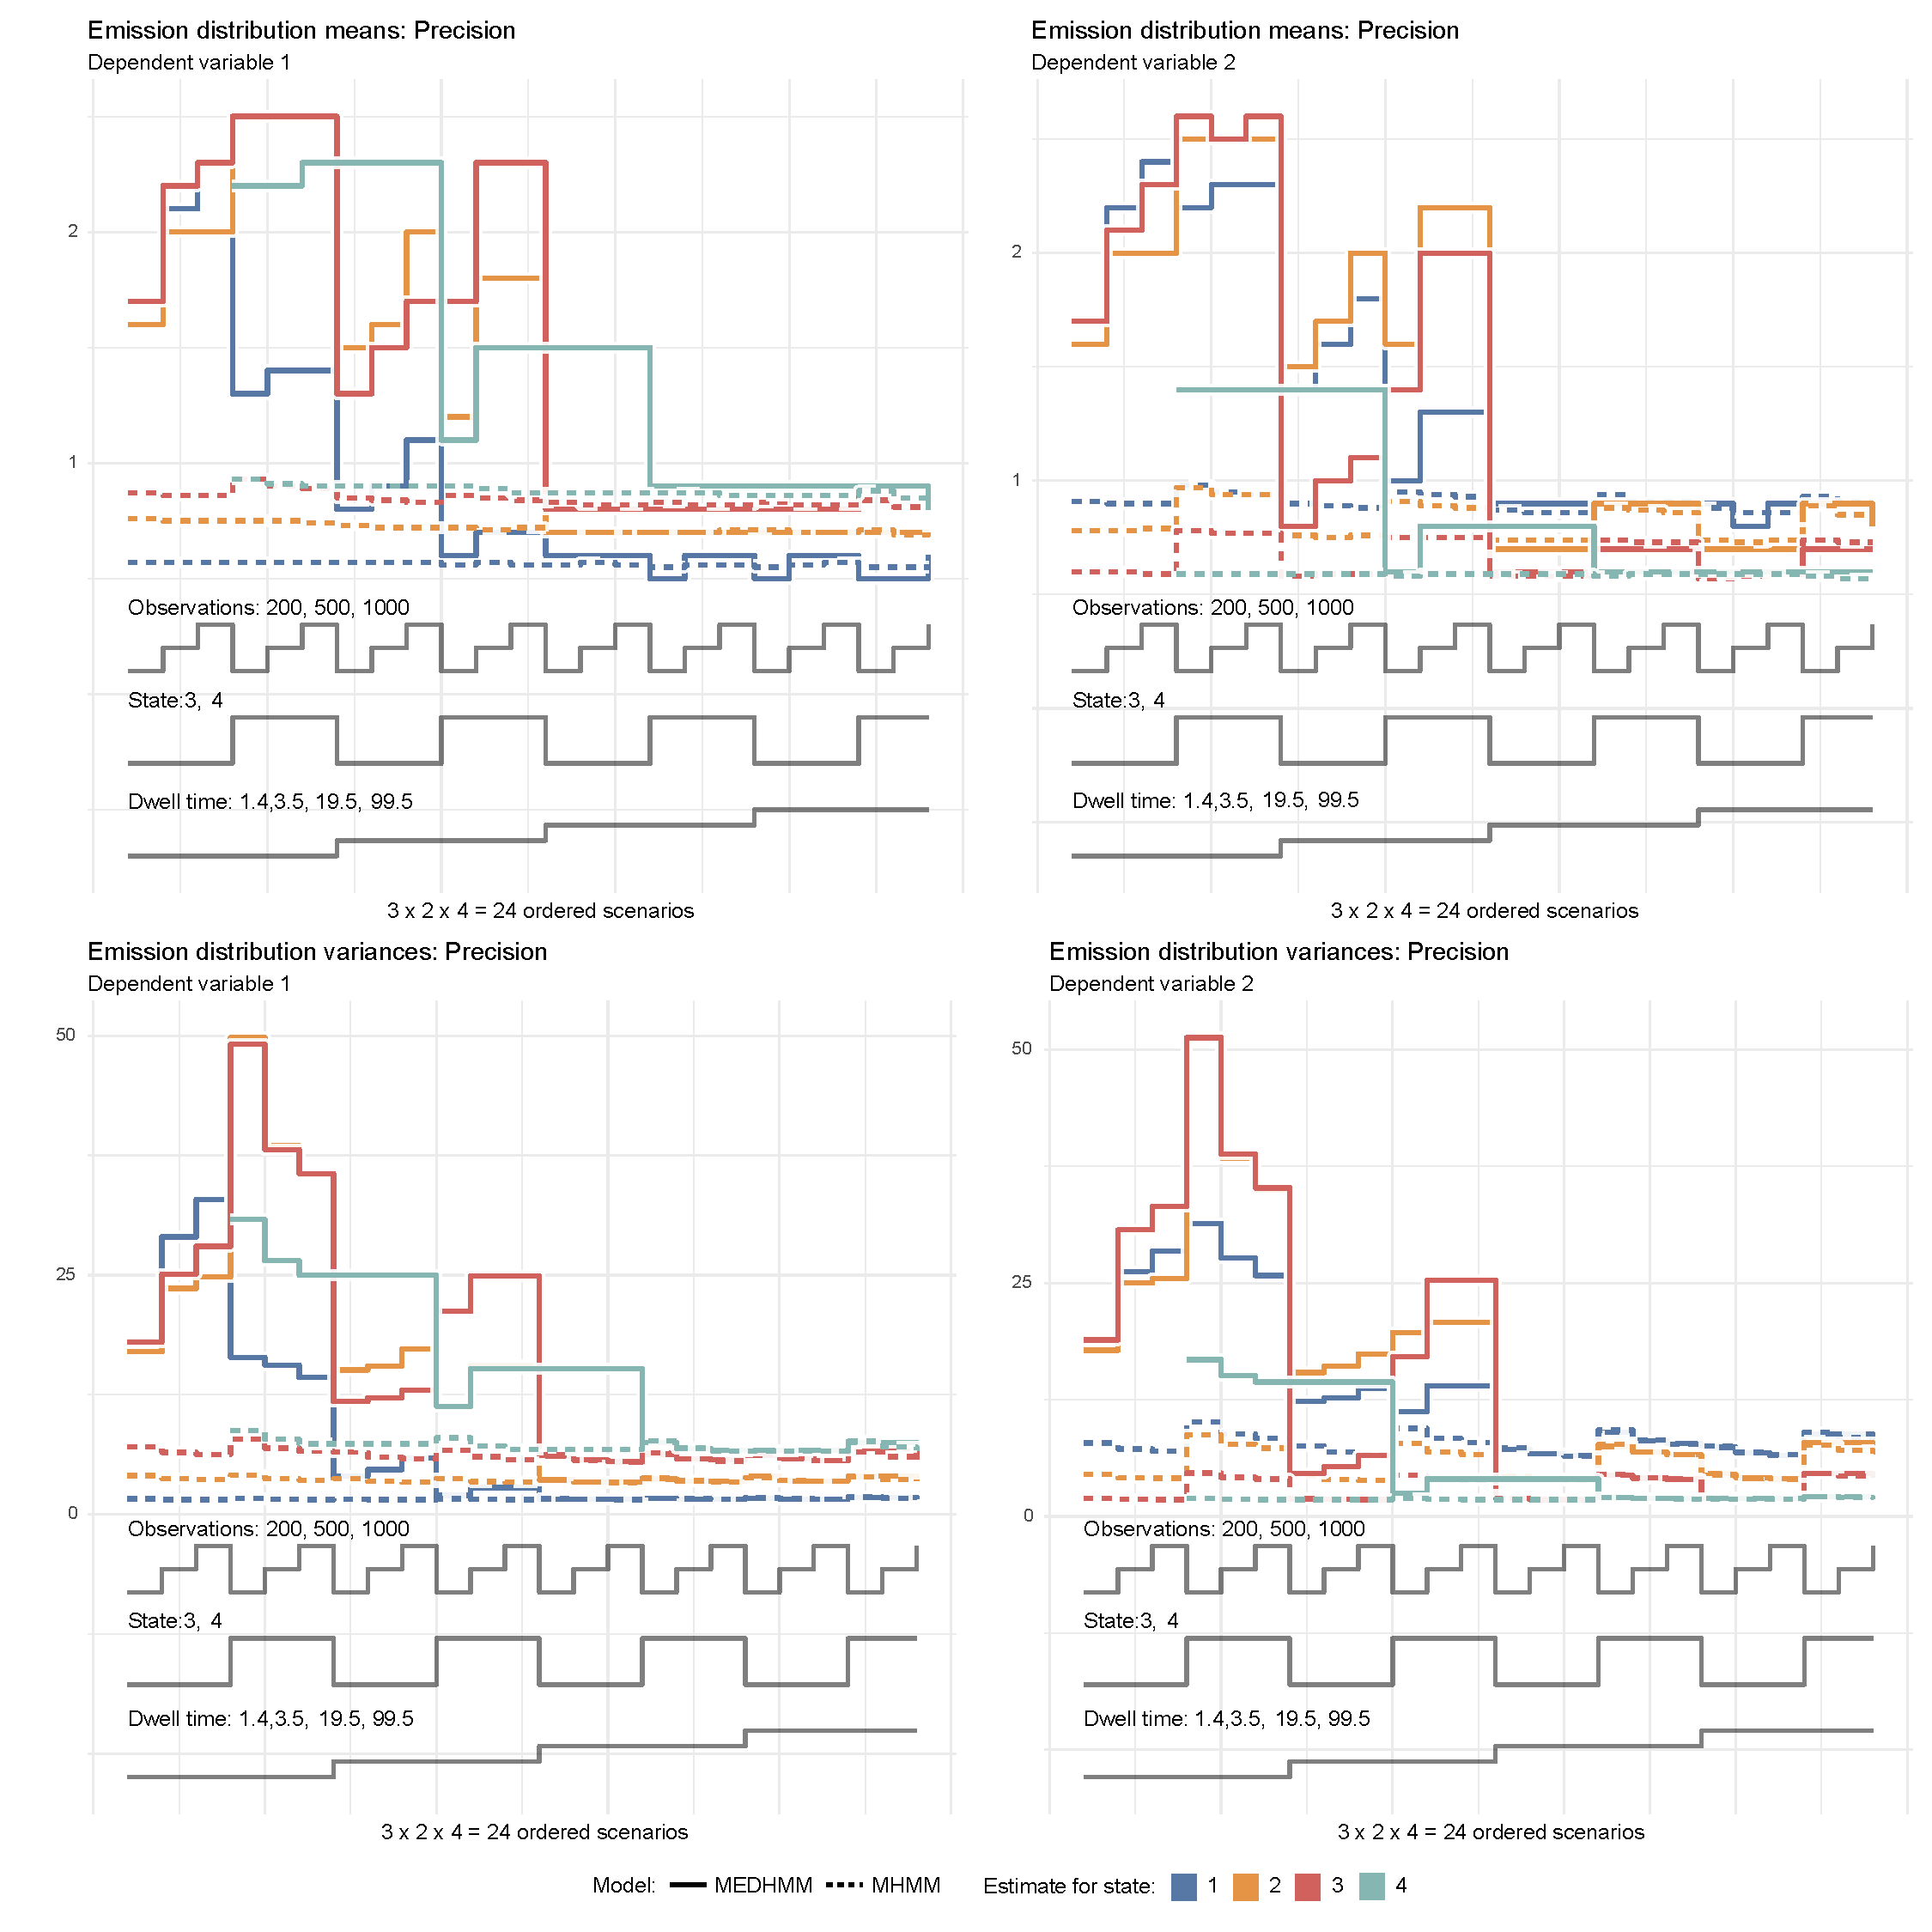
\includegraphics[width=0.75\textwidth]{graphics/emiss_sd.pdf}
    \label{prec_emiss}
    \flushleft
    \footnotesize
    \justifying
     Plots illustrate the empirical standard errors (precision) of each emission distribution means (first row) and emission variances (second row) for every simulation scenario (note that the additional scenario with varying dwell time is omitted). Each colour represent the state-specific emission mean parameters and line
type is the model indicator.
\end{figure}

%to appendix
\begin{figure}[h]
\caption{Emission distribution means: Coverage(\%)}
    \centering
    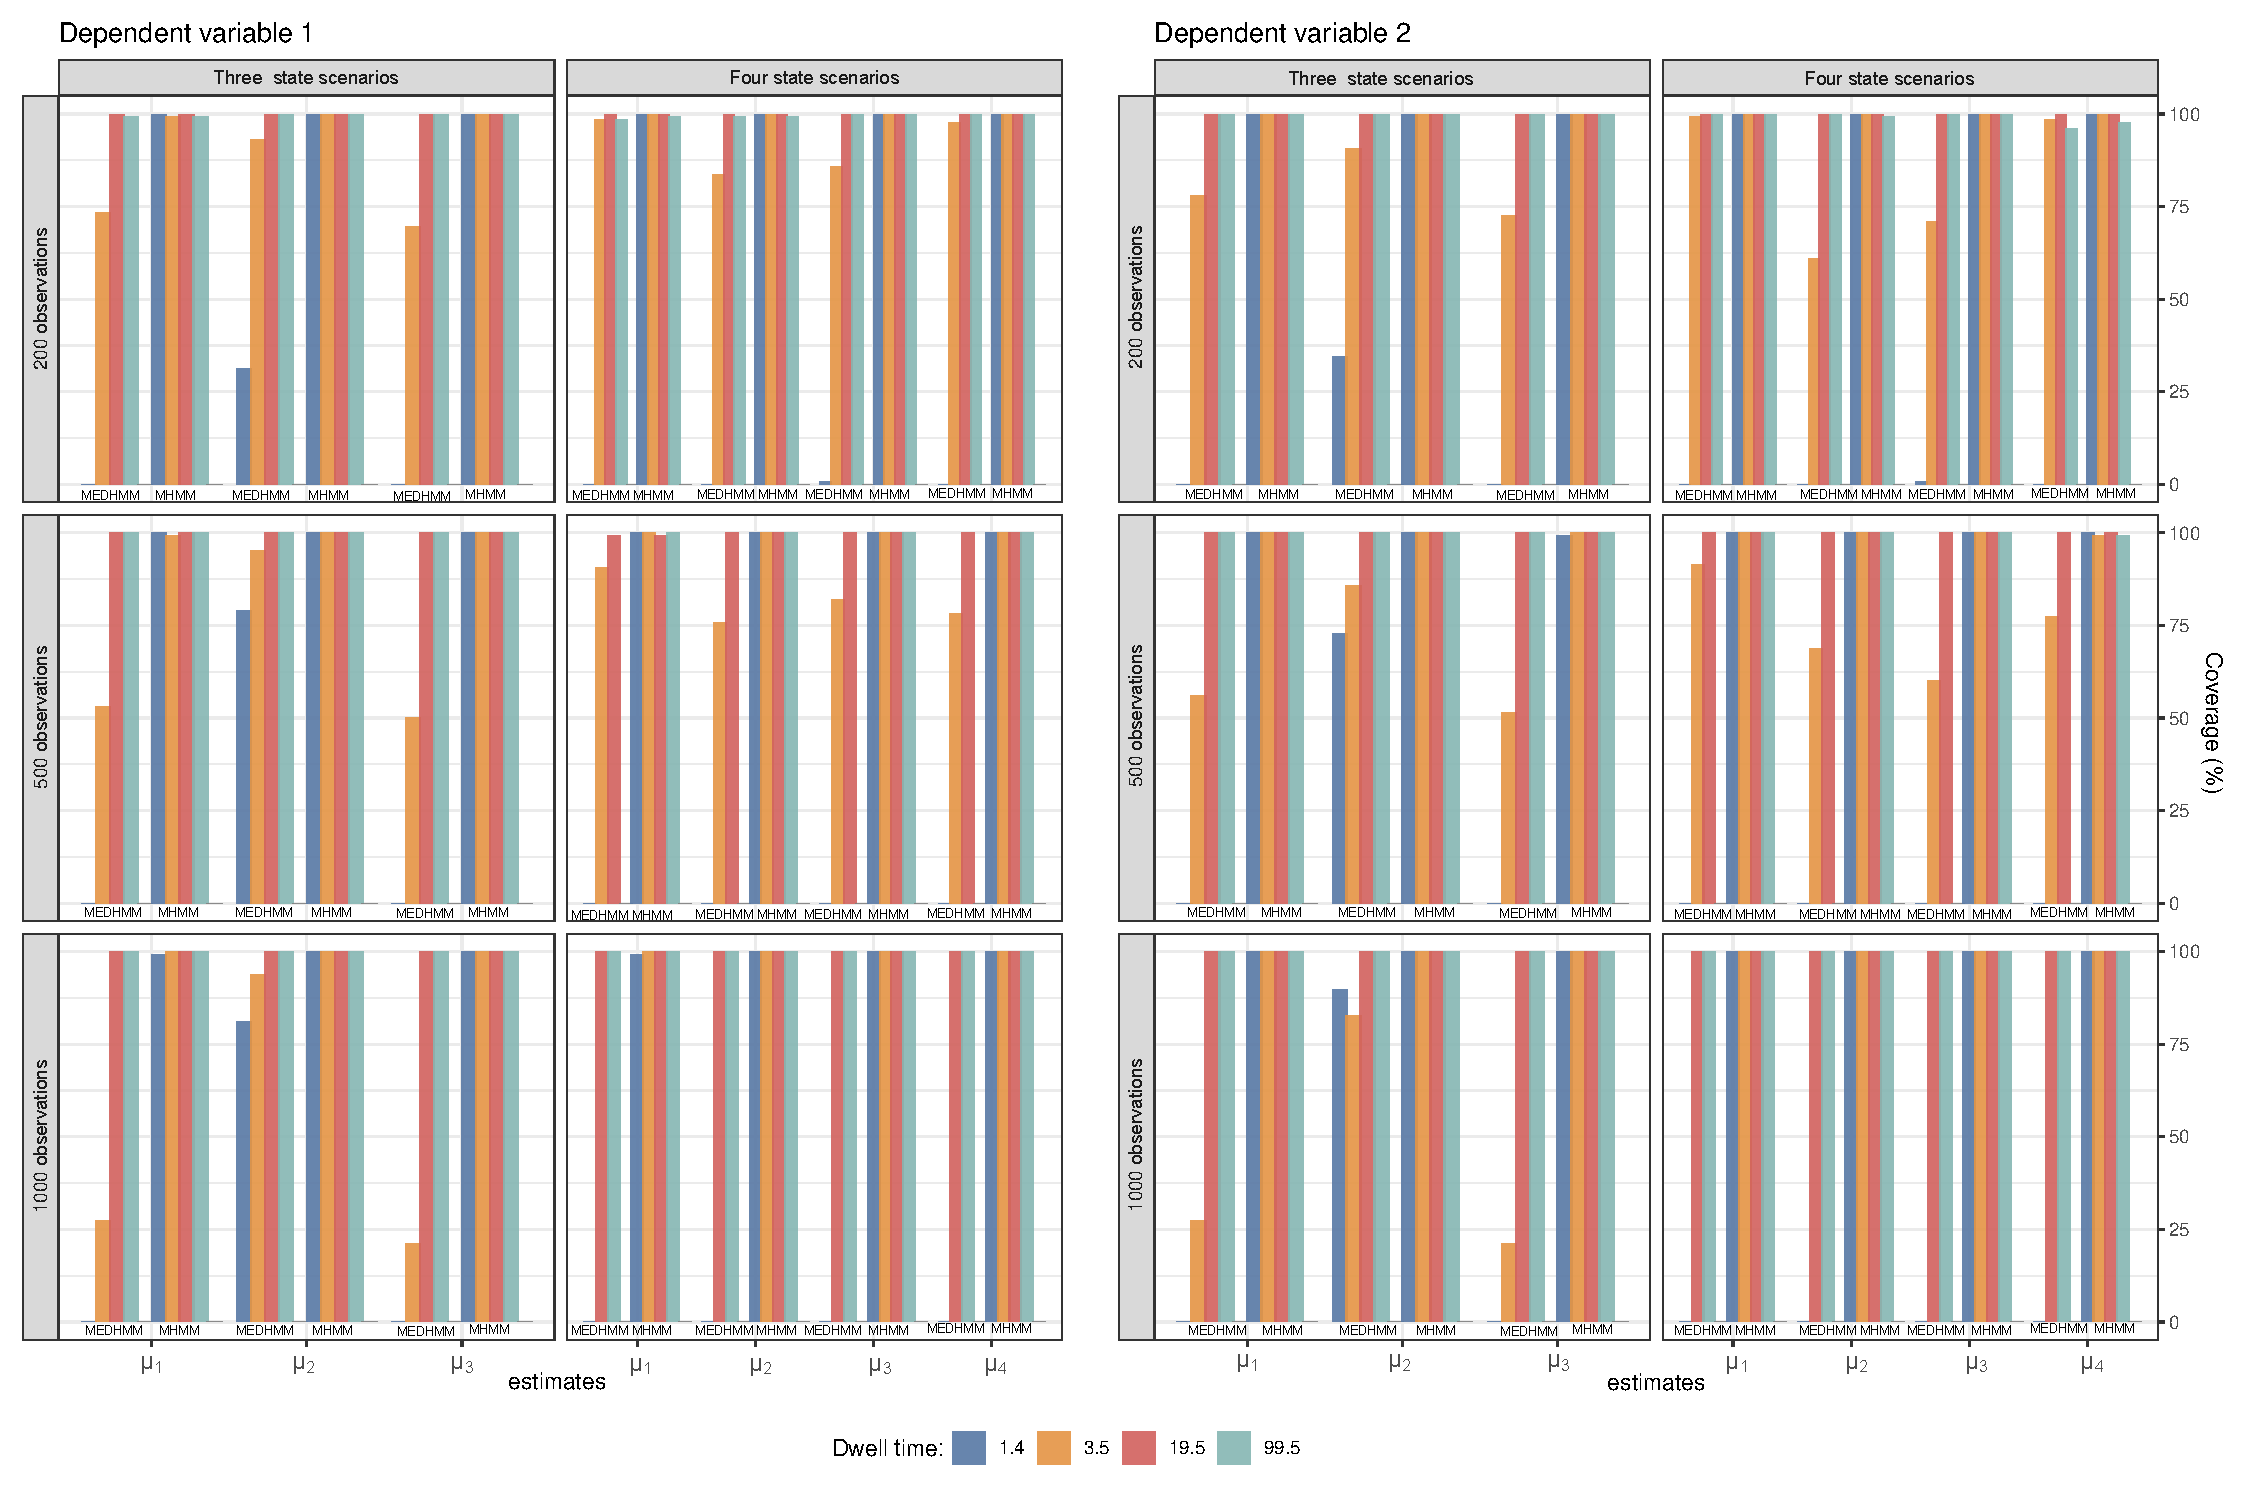
\includegraphics[width=\textwidth]{graphics/emiss_mu_cov.pdf}
     \flushleft
    \footnotesize
    \justifying
 The figure displays the Coverage over each emission distribution mean for MEDHMM and MHMM. Note that an additional scenario with varying across states dwell time was omitted here. Each panel represent a single state and observation length scenario. Colours represent the different assumed dwell time. On the x-axis the indicators of the inspected emission means are listed and within each mean parameter, the bars for MHMM and MEDHMM are shown. 
   
    \label{emiss_mu_cov}
\end{figure}



\begin{figure}[h]
\caption{The switches count for both MEDHMM \& MHMM under all simulation scenarios}
    \centering
    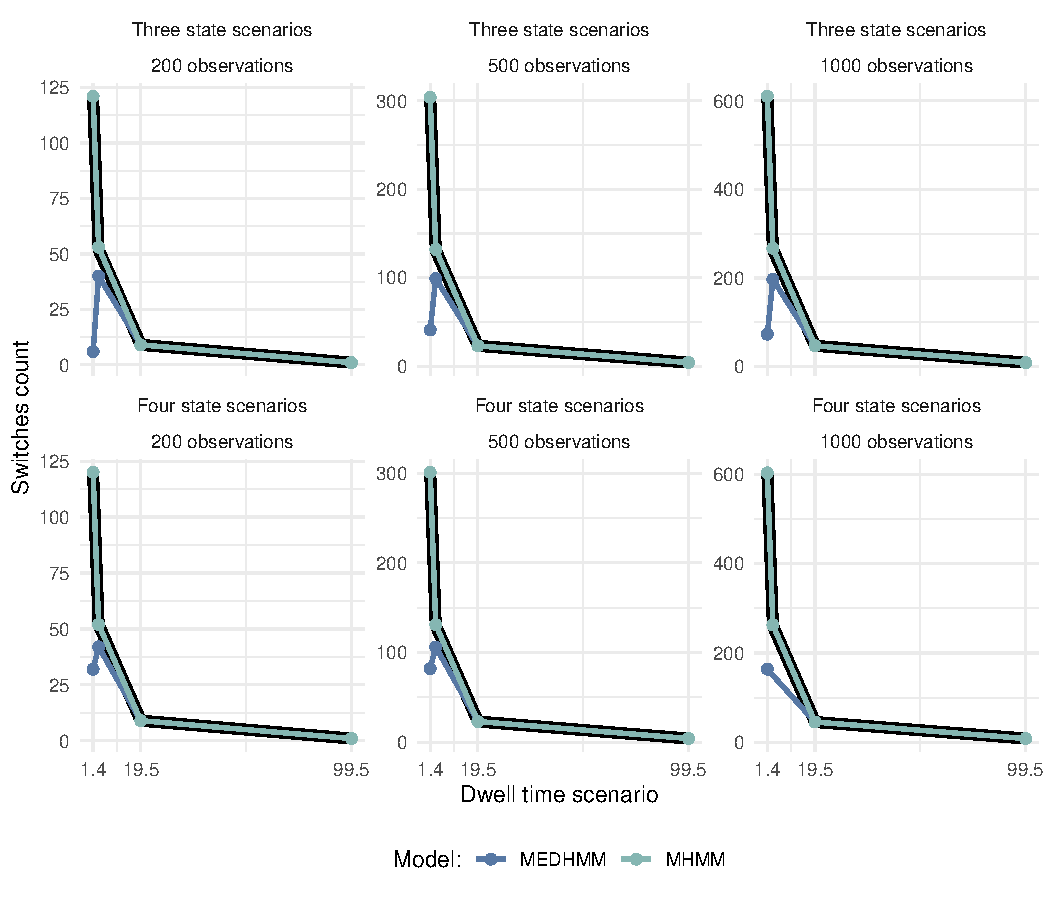
\includegraphics[width=0.9\textwidth]{graphics/switches_fin.pdf}
    \flushleft
    \footnotesize
    \justifying
    The figure displays the average count of state switches derived from local decoding (note that an additional scenario with varying across states dwell time was omitted here). Different dwell times are marked on the x-axis, and each panel represents a different observation's and state scenario. The black line indicates the in-sample true for the average number of switches.
    \label{state_switches}
\end{figure}

\begin{figure}[h]
\caption{Empirically derived dwell times}
    \centering
    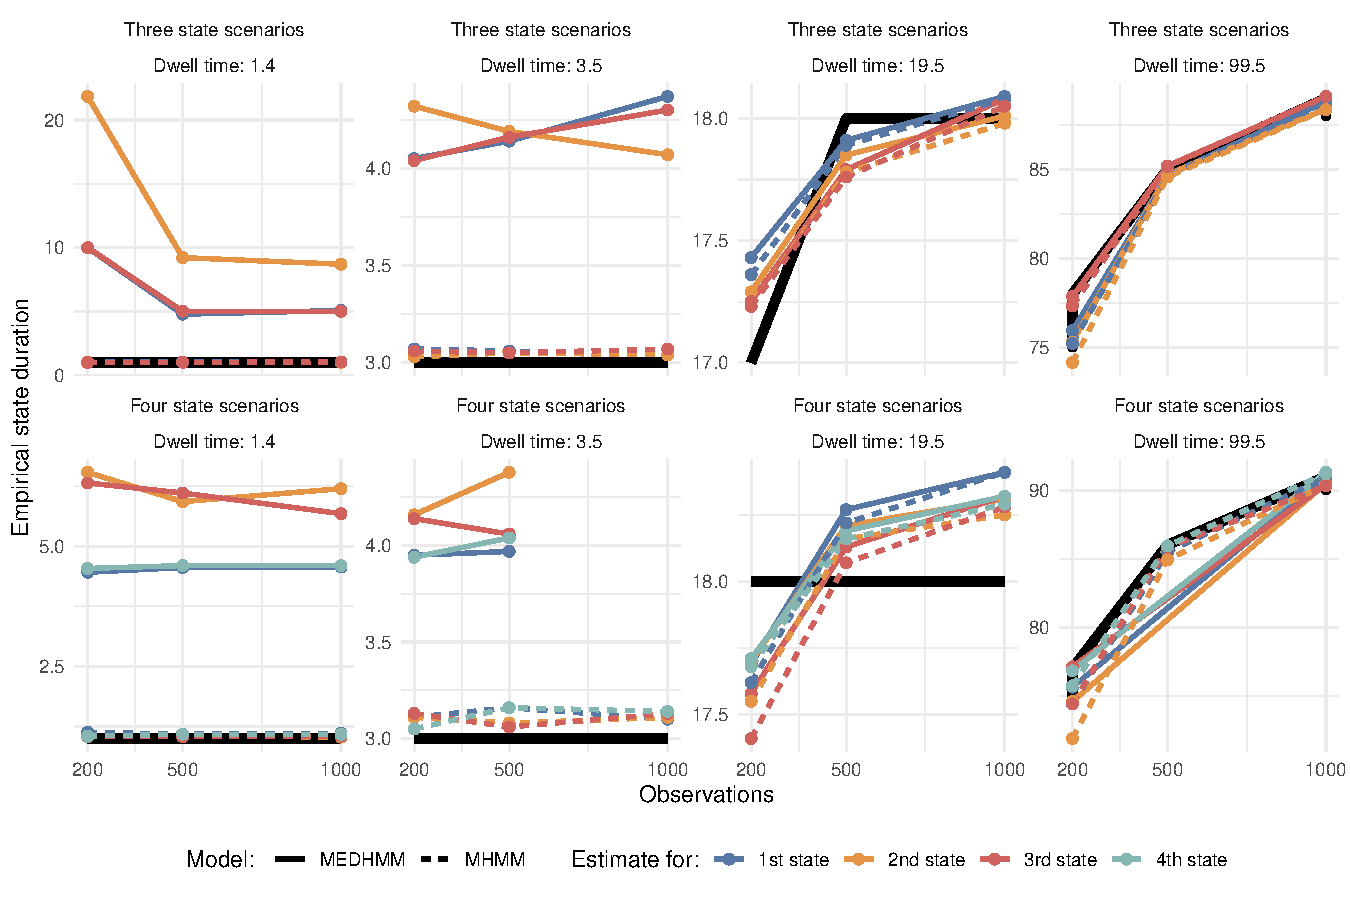
\includegraphics[width=0.8\textwidth]{graphics/dwell_time_plot.pdf}
    \flushleft
    \footnotesize
    \justifying
  The figure displays empirical state durations derived from local decoding (note that an additional scenario with varying across states dwell time was omitted here). Different lengths of observations are marked on the x-axis, and each panel represents a different dwell time and state scenario. The black line shows the average true empirical dwell time across all states, while each coloured line represents a state-specific dwell time estimate. Different models are indicated by the line type. 
    \label{empiric_dwell}
\end{figure}



%% % \usepackage{booktabs}


% \begin{table}
% \centering
% \caption{Maximum a posteriori results for the additional simulation scenario}
% \label{mixed_sim}
% \resizebox{\linewidth}{!}{
% \begin{tabular}{crcccccccccc} 
% \toprule
% \multicolumn{2}{r}{~} & \multicolumn{5}{c}{MEDHMM} & \multicolumn{5}{c}{MHMM} \\ 
% \cmidrule(lr){3-7}\cmidrule(lr){8-12}
% distribution & \multicolumn{1}{c}{parameter} & TRUE & Median (ESE) & Bias & Bias (\%)* & Coverage (\%) & TRUE & Median (ESE) & Bias & Bias (\%)* & Coverage (\%) \\ 
% \midrule
% emisssion distribution & $\bar{\mu_{11}}$ & 10 & 10.8 (0.6) & 0.8 & 8.5 & 79.7 & 10 & 10.12 (0.6) & 0.12 & 1.22 & 100 \\
%  & $\bar{\mu_{12}}$ & 30 & 30 (0.7) & 0 & 1 & 100 & 30 & 30.02 (0.7) & 0.02 & 0.06 & 100 \\
%  & $\bar{\mu_{13}}$ & 60 & 60 (0.8) & 0 & 0.1 & 100 & 60 & 59.96 (0.8) & -0.04 & 0.07 & 100 \\
%  & $\bar{\mu_{21}}$ & 60 & 58.5 (1.1) & -1.5 & 2.5 & 79.7 & 60 & 59.75 (1.0) & -0.25 & 0.42 & 100 \\
%  & $\bar{\mu_{22}}$ & 30 & 30 (0.7) & 0 & 0.1 & 100 & 30 & 29.97 (0.7) & -0.03 & 0.09 & 100 \\
%  & $\bar{\mu_{23}}$ & 10 & 10 (0.6) & 0 & 0.4 & 100 & 10 & 10.04 (0.6) & 0.04 & 0.39 & 100 \\
%  & \sigma^2_{11} & 20 & 35.1 (3.6) & 15.1 & 75.4 & 0 & 20 & 26.3 (2.0) & 6.3 & 31.48 & 0 \\
%  & \sigma^2_{12} & 60 & 74.4 (3.7) & 14.4 & 24.1 & 0 & 60 & 73.37 (3.7) & 13.37 & 22.28 & 0 \\
%  & \sigma^2_{13} & 120 & 140.8 (5.4) & 20.8 & 17.3 & 0 & 120 & 140.91 (5.4) & 20.91 & 17.42 & 0 \\
%  & \sigma^2_{21} & 150 & 188.3 (12.4) & 38.3 & 25.5 & 9.4 & 150 & 169.24 (10.4) & 19.24 & 12.83 & 42.19 \\
%  & \sigma^2_{22} & 75 & 91.8 (4.4) & 16.8 & 22.4 & 0 & 75 & 90.09 (4.3) & 15.09 & 20.12 & 0 \\
%  & \sigma^2_{23} & 25 & 33.6 (1.8) & 8.5 & 34.5 & 0 & 25 & 33.6 (1.8) & 8.6 & 34.4 & 0 \\ 
% \midrule
% gamma distribution & \gamma_{11} & - & - & - & - & - & 0.75 & 0.65 (0.02) & -0.1 & 12.8 & 0 \\
%  & \gamma_{12} & 0.5 & 0.5 (0.0) & 0 & 3.4 & 95.3 & 0.125 & 0.18 (0.01) & 0.05 & 41.18 & 0.78 \\
%  & \gamma_{13} & 0.5 & 0.5 (0.0) & 0 & 3.4 & 95.3 & 0.125 & 0.17 (0.01) & 0.04 & 35.3 & 2.34 \\
%  & \gamma_{21} & 0.5 & 0.5 (0.0) & 0 & 8.1 & 84.4 & 0.025 & 0.04 (0.0) & 0.01 & 55.36 & 0 \\
%  & \gamma_{22} & - & - & - & - & - & 0.95 & 0.92 (0.01) & -0.03 & 2.75 & 0 \\
%  & \gamma_{23} & 0.5 & 0.5 (0.0) & 0 & 8.1 & 84.4 & 0.025 & 0.04 (0.0) & 0.01 & 48.63 & 1.56 \\
%  & \gamma_{31} & 0.5 & 0.5 (0.0) & 0 & 4.3 & 93 & 0.005 & 0.01 (0.0) & 0 & 43.49 & 0.78 \\
%  & \gamma_{32} & 0.5 & 0.5 (0.0) & 0 & 4.3 & 93 & 0.005 & 0.01 (0.0) & 0 & 43.18 & 2.34 \\
%  & \gamma_{33} & - & - & - & - & - & 0.99 & 0.99 (0.0) & 0 & 0.44 & 0 \\ 
% \midrule
% dwell time distribution & $\bar{\mu_{[d]1}}$ & 1.2 & 1.4 (0.0) & 0.1 & 9.7 & 21.1 & - & - & - & - & - \\
%  & $\bar{\mu_{[d]2}}$ & 3 & 3 (0.1) & 0 & 0.2 & 93.8 & - & - & - & - & - \\
%  & $\bar{\mu_{[d]3}}$ & 4.6 & 4.6 (0.0) & 0 & 0.5 & 93 & - & - & - & - & - \\
%  & $\bar{\sigma^2_{[d]1}}$ & 0.1 & 0.1 (0.0) & 0 & 3.8 & 95.3 & - & - & - & - & - \\
%  & $\bar{\sigma^2_{[d]2}}$ & 0.1 & 0.1 (0.0) & 0 & 1.9 & 95.3 & - & - & - & - & - \\
%  & $\bar{\sigma^2_{[d]3}}$ & 0.1 & 0.1 (0.0) & 0 & 1.6 & 95.3 & - & - & - & - & - \\
% \bottomrule
% \multicolumn{9}{l}{*The values presented are absolute values of the \%Bias.}
% \end{tabular}
% }
% \end{table}




\section{Empirical example: Selected results}
\begin{figure}[h]
\centering
\caption{Empirical example: Posterior predictive checks (PPCs) for MEDHMM}
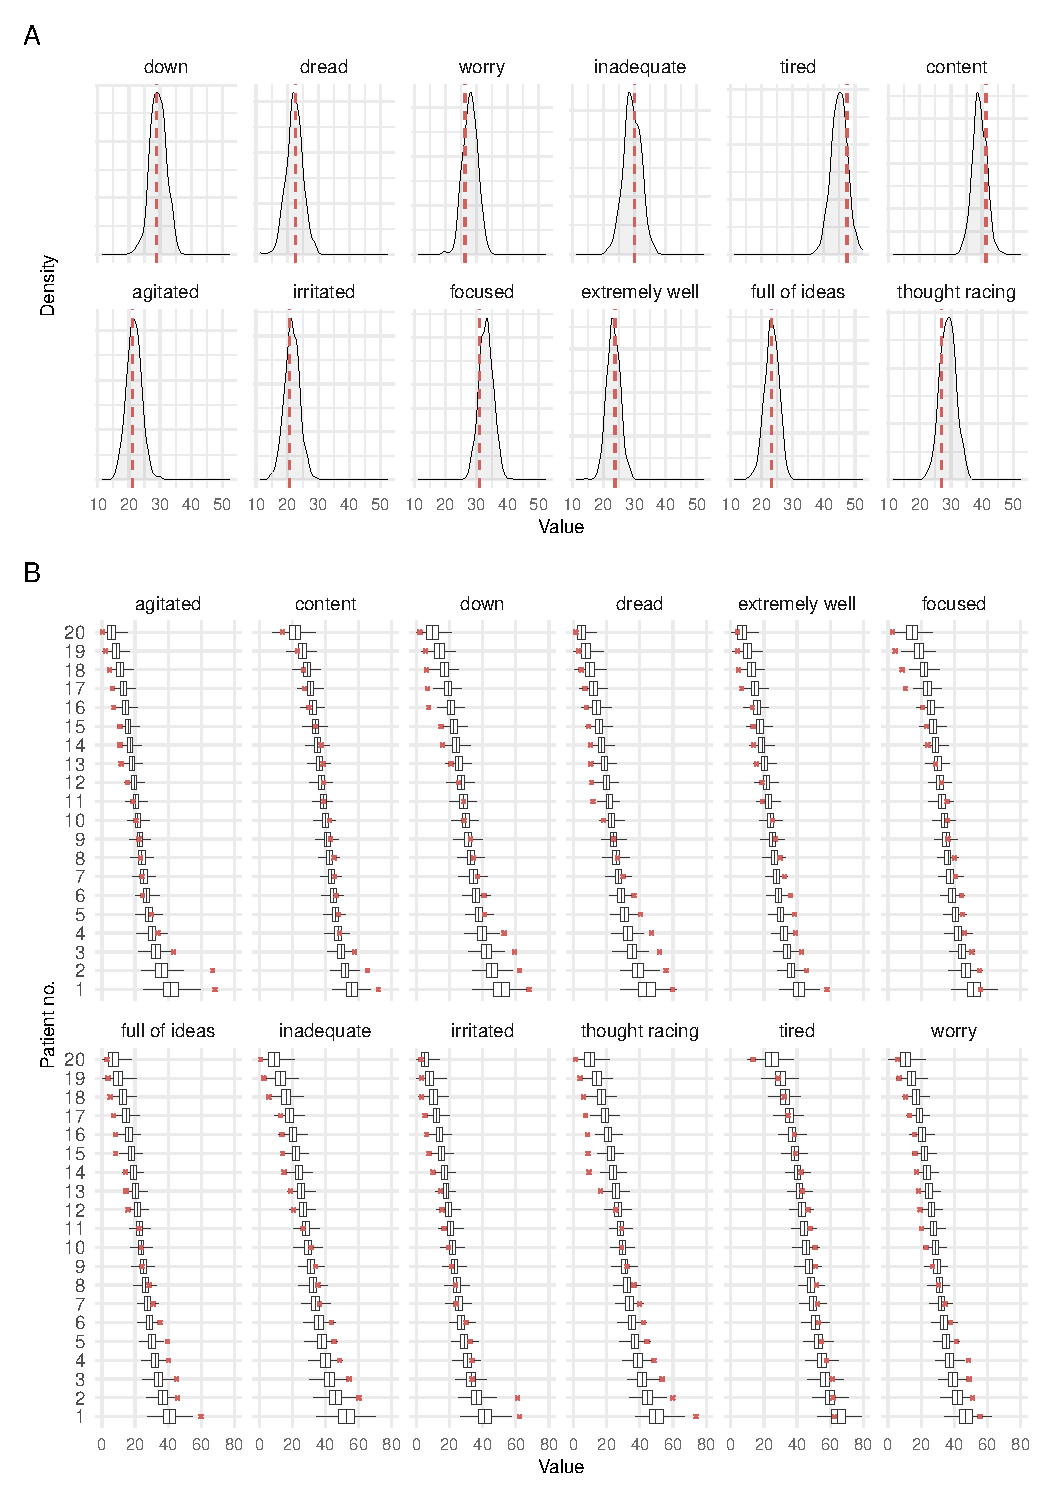
\includegraphics[width=0.7\textwidth]{graphics/ppc_mean_emiss.pdf}
\flushleft
\footnotesize
\justifying
 Panel A represent the group-level emission distribution scores on considered items observed in the data (red dashed line) and the distribution of scores multiply sampled from the MEDHMM (shaded grey distributions). Panel B represent the subject-level emission distribution mean scores on considered items observed in the data (red crosses) and the distribution of scores multiply sampled from the MEDHMM (boxplots).\label{ppc_out_mean_medhmm}
\end{figure}

\begin{figure}[h]
\centering
\caption{Empirical example: Posterior predictive checks (PPCs) for MHMM}
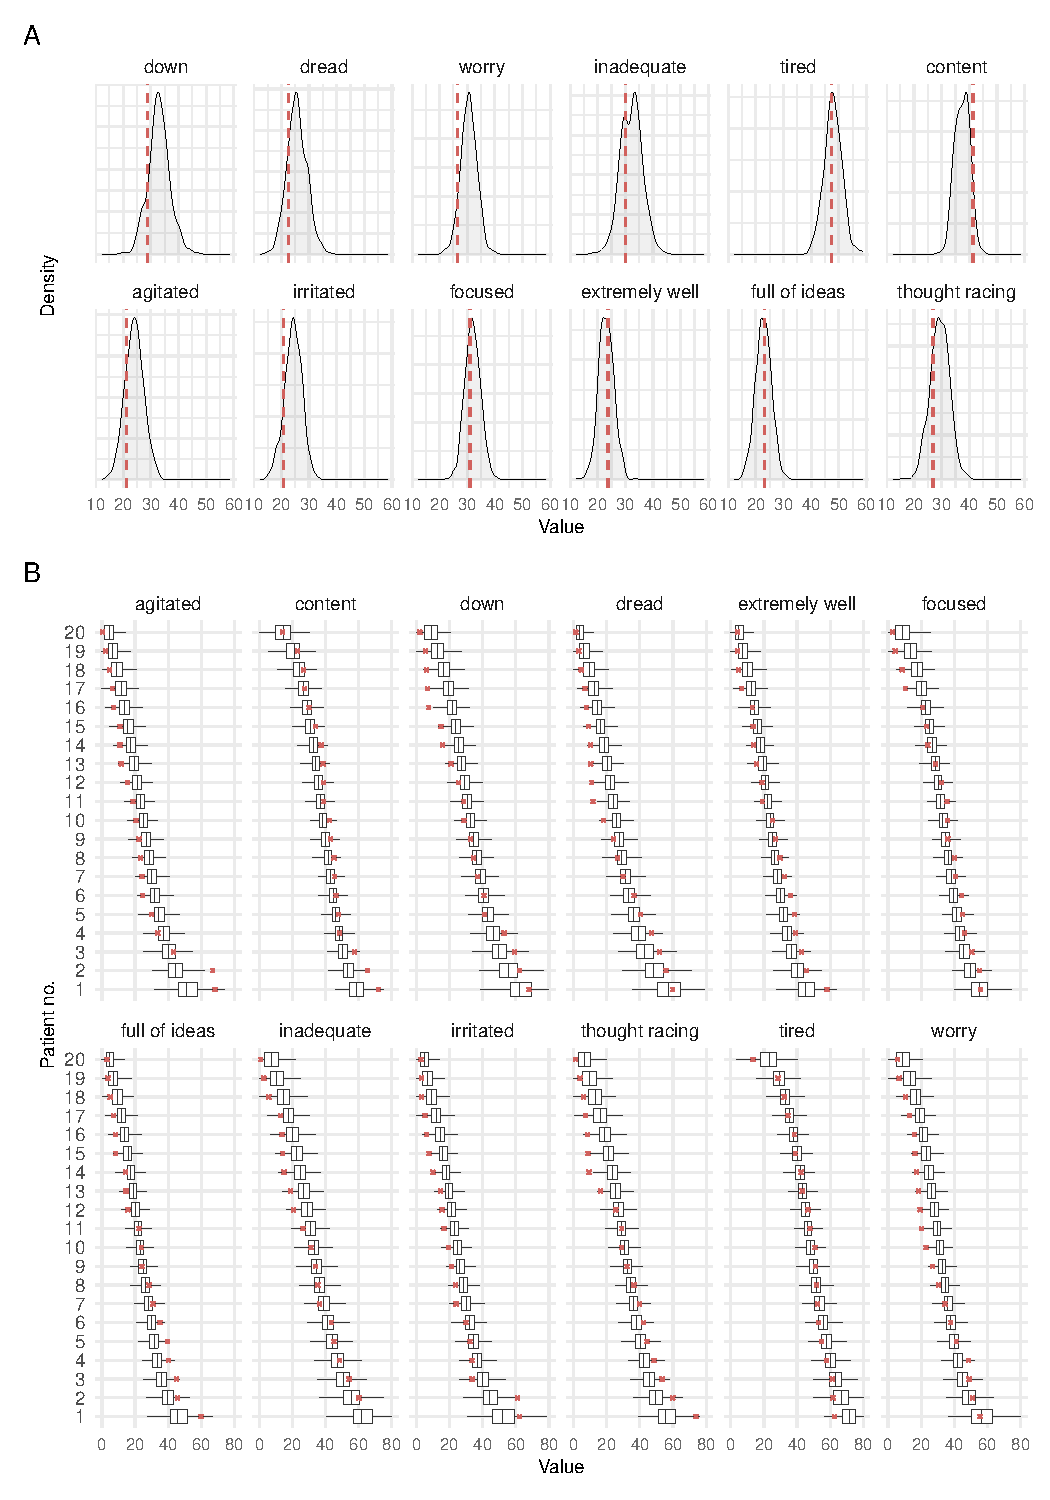
\includegraphics[width=0.8\textwidth]{graphics/ppc_mean_hmm.pdf}
\flushleft
\footnotesize
\justifying
 Panel A represent the group-level emission distribution scores on considered items observed in the data (red dashed line) and the distribution of scores multiply sampled from the MHMM (shaded grey distributions). Panel B represent the subject-level emission distribution of mean scores on considered items observed in the data (red crosses) and the distribution of scores multiply sampled from the MEDHMM (boxplots). 
 \label{ppc_out_mean_mhmm}
\end{figure}


\begin{figure}[h]
\caption{Empirical example: The group-level MHMM transition probability matrix}
    \centering
    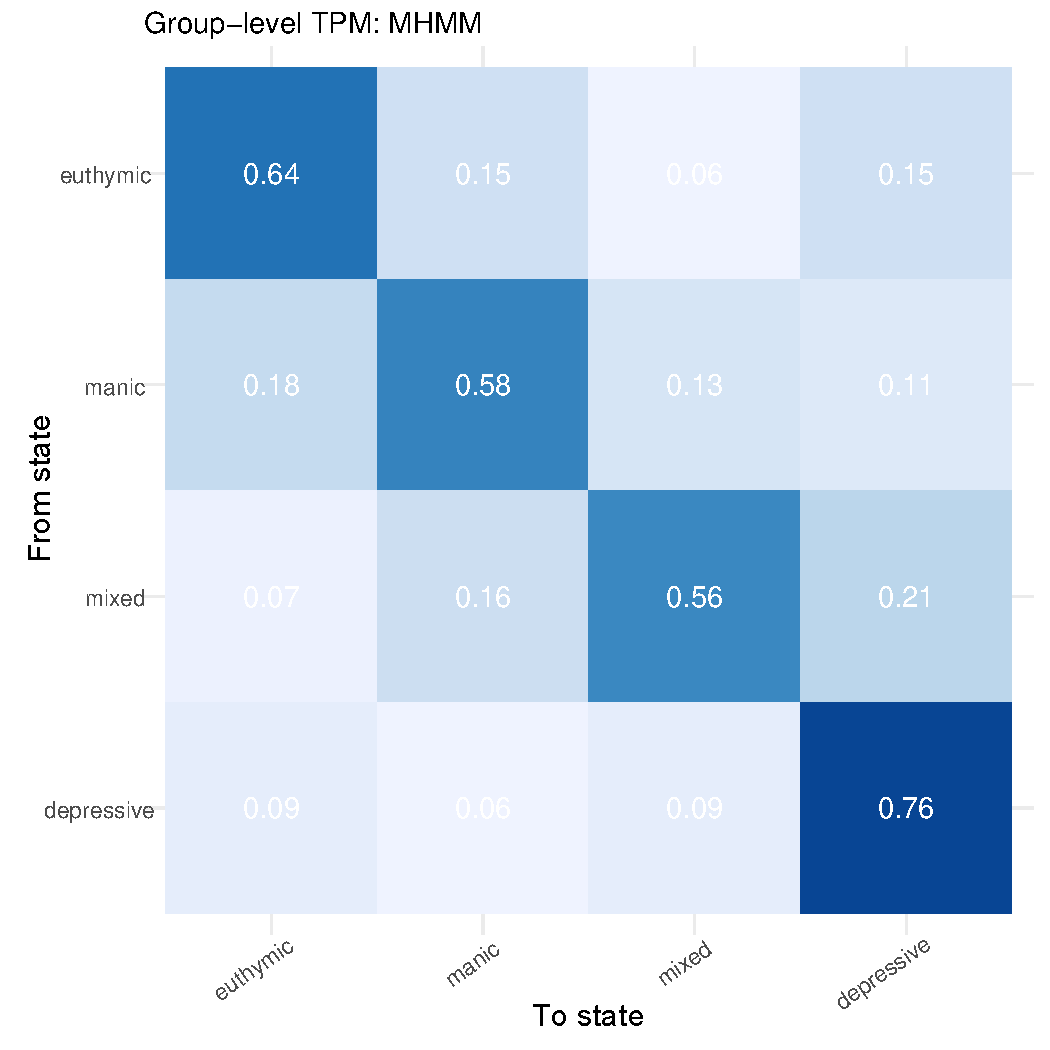
\includegraphics[width=0.65\linewidth]{graphics/group_trandition_matricesvv2.pdf}
    \label{emp_group_trans}
\end{figure}

\begin{sidewaysfigure}
    \centering    
    \caption{Empirical example: Comparison of group-level emission distribution means and variances estimates for the MEDHMM and MHMM}
 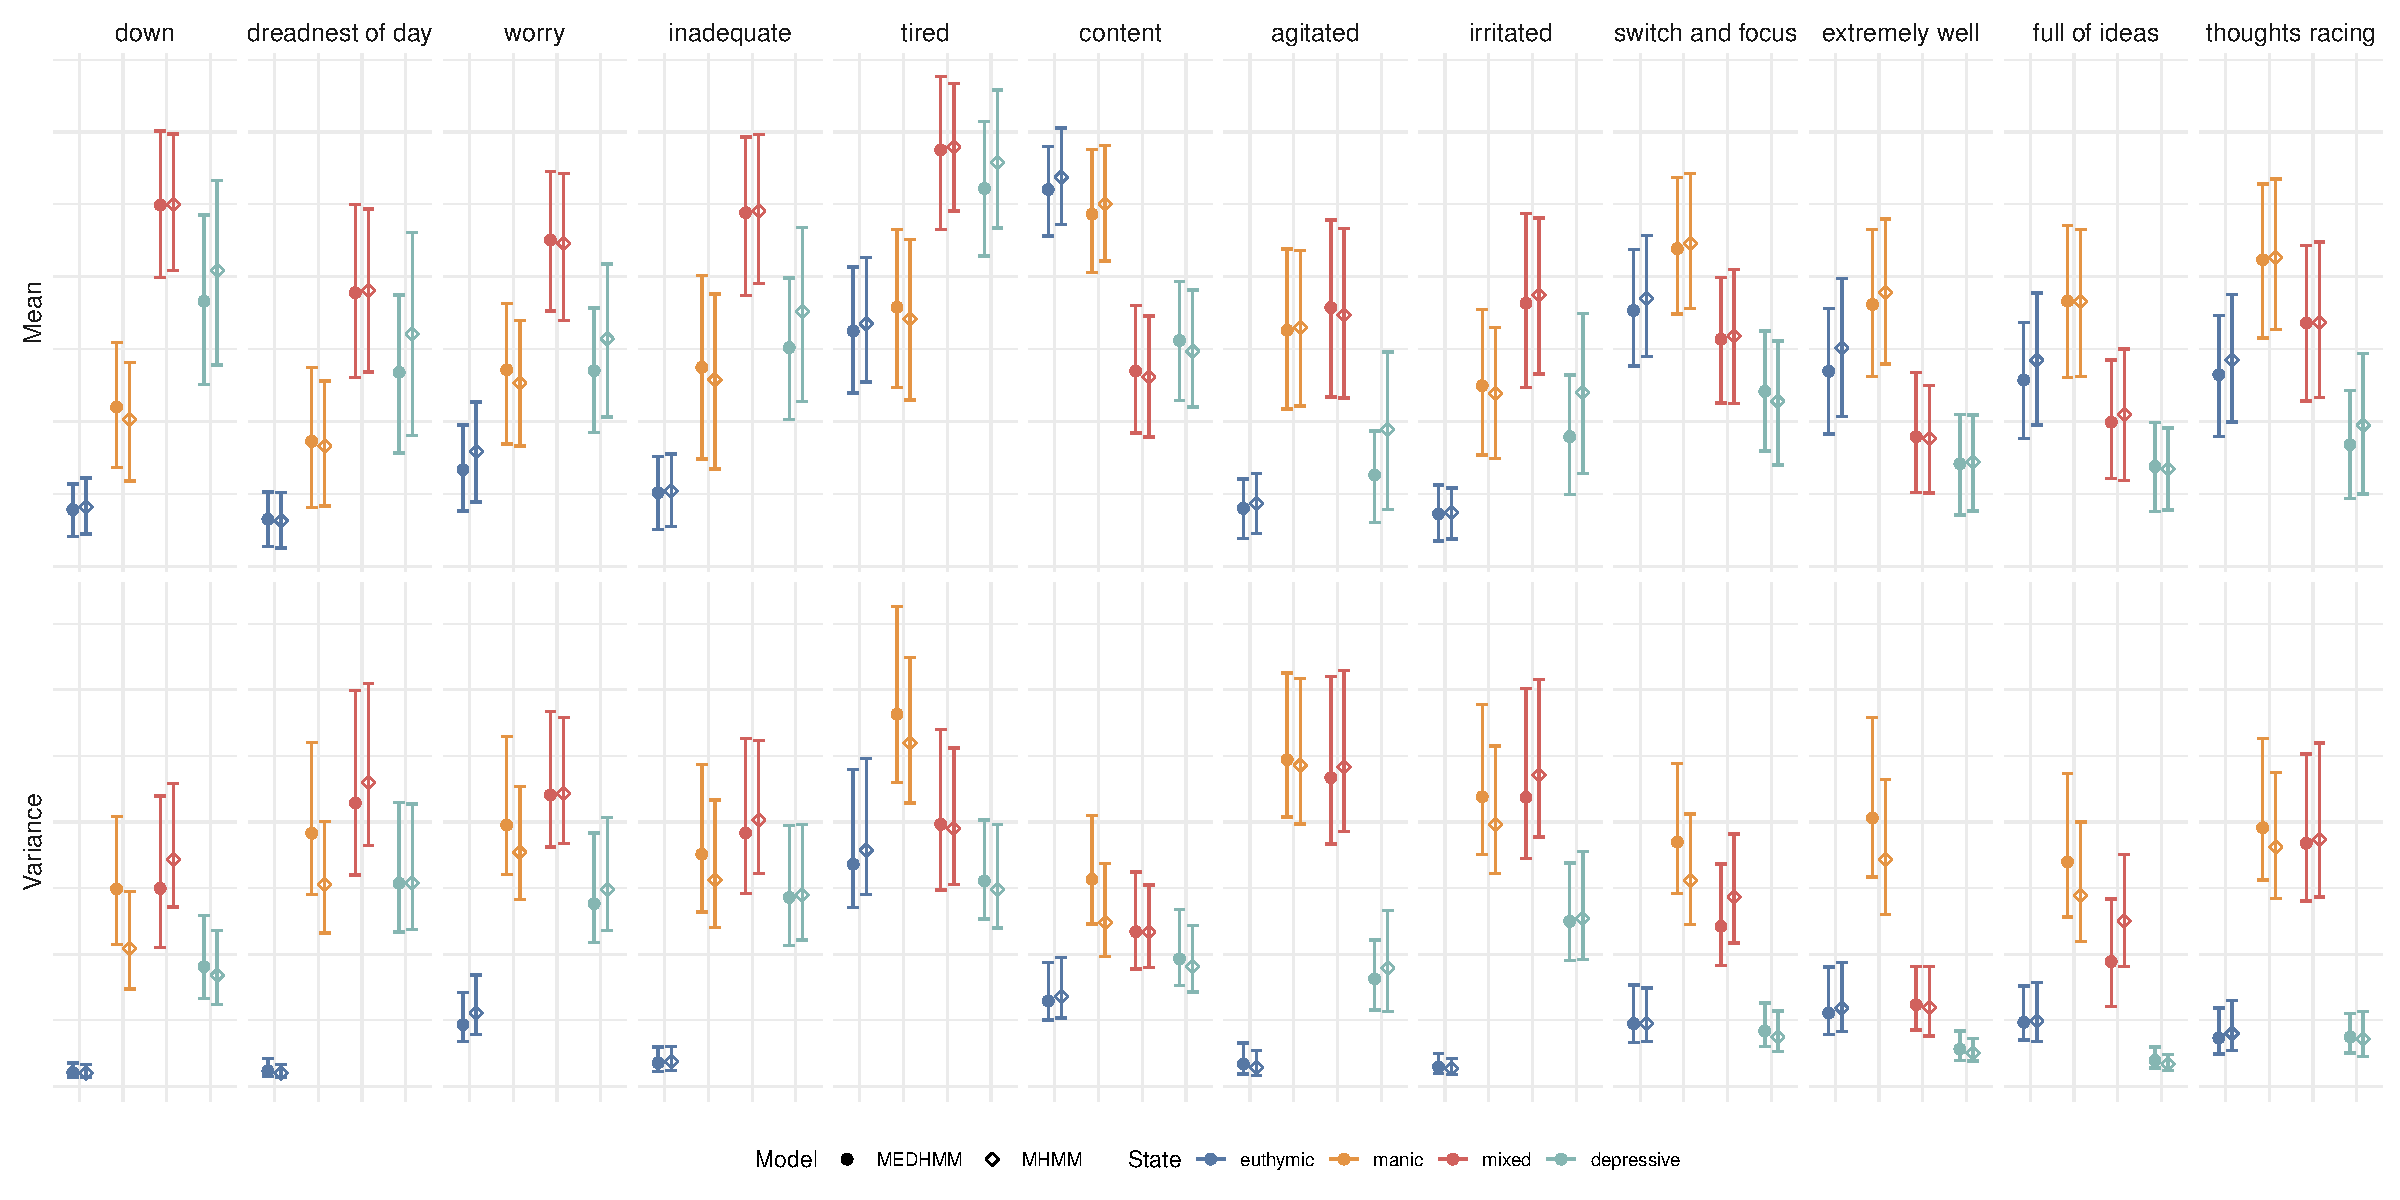
\includegraphics[scale=0.6]{graphics/comparison_emiss_group_level2.pdf}
 \flushleft
 \footnotesize
 \justifying
 This figure shows comparison between group-level estimates of emission distribution parameters. The first row contains estimates for emission means, and the second row shows the emission variances. Each vertical panel represents a dependent variable (inspected EMA item). Within each plot for dependent variable parameters, each Bipolar disorder mood state-specific estimate is marked with a different colour. The round points are indicators of MHMM and diamond points are the MEDHMM estimates. 
    \label{group_emission_emp}
\end{sidewaysfigure}

\begin{figure}
    \centering    
    \caption{Empirical example: Temporal alignment between mood states and weekly symptom scores}
 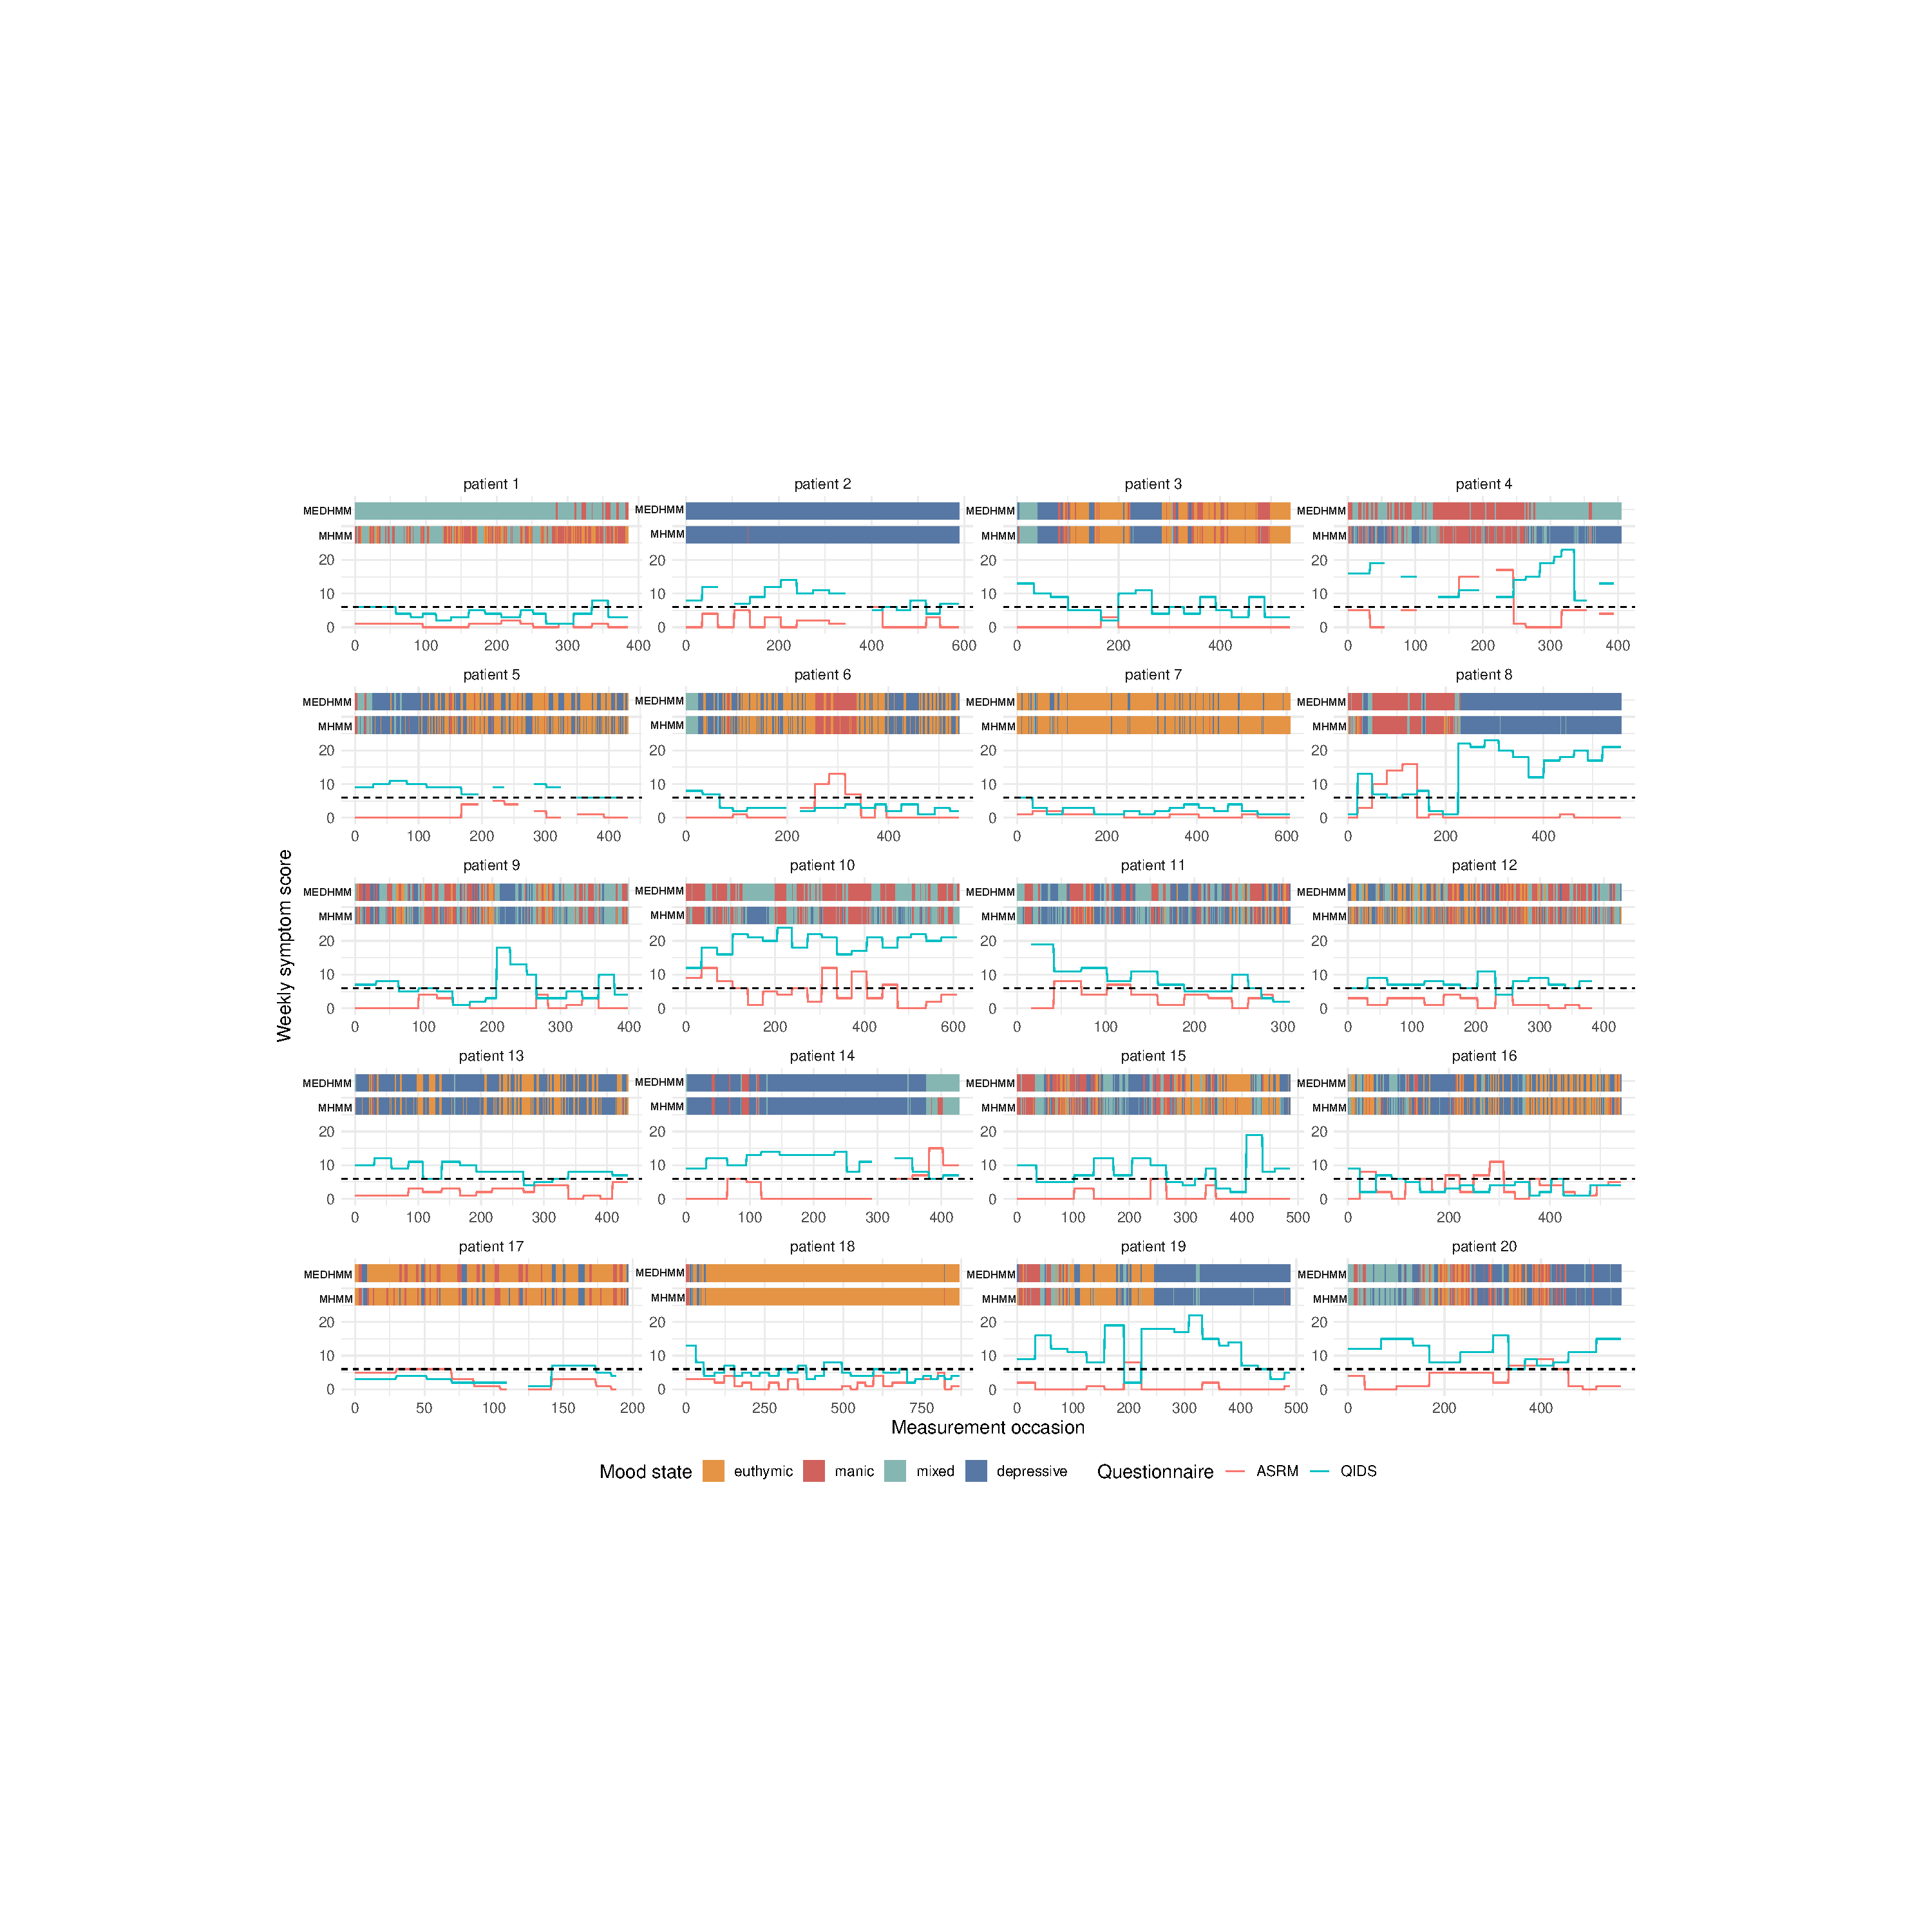
\includegraphics[width=\linewidth]{graphics/decoding_all.pdf}
 \flushleft
 \footnotesize
 The figure shows local state decodings for the MEDHMM (upper decoding strip) and the MHMM (lower decoding script). The plots are presented for all Bipolar disorder patients. Under the strip plots the alignment with the weekly symptom scores on depressive behaviour indicator (QIDS) and manic behaviour indicator (ASRM).
    \label{decoding_all}
\end{figure}

% Please add the following required packages to your document preamble:
% \usepackage{booktabs}
% \usepackage{lscape}

\begin{table}[h]
\caption{Empirical example: Analysis of switches between states \& empirically assessed average state durations}
\resizebox{\linewidth}{!}{
\begin{tabular}{cccccccc}
  \toprule
   &  & \multicolumn{6}{c}{MEDHMM}\\ \cmidrule{3-8}
\textbf{Patient no.} &
 \textbf{Observations} &
 \textbf{Switches count} &
  \textbf{Relative proportion of switches} &
  \textbf{Euthymic state} &
  \textbf{Manic state} &
  \textbf{Mixed state} &
  \textbf{Depressive state}  \\ \midrule

1 & 386 & 16 & 0.041 & 4.83 & 5.71 & 6.69 & 5.10 \\
2 & 589 & 0 & 0 & 4.79 & 4.29 & 4.41 & 5.07 \\
3 & 538 & 61 & 0.113 & 6.84 & 3.27 & 4.82 & 7.10 \\
4 & 405 & 41 & 0.101 & 4.91 & 4.82 & 4.23 & 5.15 \\
5 & 431 & 71 & 0.165 & 5.03 & 2.94 & 4.74 & 4.81 \\
6 & 540 & 83 & 0.154 & 4.92 & 8.18 & 5.20 & 4.13 \\
7 & 608 & 47 & 0.077 & 13.32 & 4.30 & 4.08 & 2.91 \\
8 & 559 & 16 & 0.029 & 4.31 & 11.25 & 4.43 & 8.36 \\
9 & 399 & 99 & 0.248 & 3.41 & 3.42 & 4.03 & 3.41 \\
10 & 613 & 50 & 0.082 & 4.78 & 7.68 & 5.81 & 5.04 \\
11 & 308 & 84 & 0.273 & 2.75 & 3.85 & 3.96 & 4.14 \\
12 & 427 & 115 & 0.269 & 2.99 & 3.80 & 3.69 & 3.43 \\
13 & 434 & 60 & 0.138 & 3.92 & 3.60 & 4.11 & 6.45 \\
14 & 428 & 16 & 0.037 & 4.83 & 5.14 & 3.59 & 17.90 \\
15 & 486 & 95 & 0.195 & 4.28 & 3.87 & 3.83 & 3.63 \\
16 & 541 & 111 & 0.205 & 3.60 & 3.58 & 4.00 & 4.57 \\
17 & 197 & 44 & 0.223 & 5.20 & 2.67 & 4.24 & 3.13 \\
18 & 869 & 13 & 0.015 & 11.89 & 4.84 & 4.07 & 4.27 \\
19 & 489 & 40 & 0.082 & 5.56 & 5.15 & 4.03 & 6.26 \\
20 & 566 & 95 & 0.168 & 3.41 & 3.42 & 4.59 & 5.91 \\
\bottomrule
\end{tabular}}


\resizebox{\linewidth}{!}{
\begin{tabular}{cccccccc}
  \toprule
   & &  \multicolumn{6}{c}{MHMM}\\ \cmidrule{3-8}
\textbf{Patient no.} &
 \textbf{Observations} &
  \textbf{Switches count} &
  \textbf{Relative proportion of switches} &
  \textbf{Euthymic state} &
  \textbf{Manic state} &
 \textbf{Mixed state} &
  \textbf{Depressive state} \\ \midrule
1 & 386 & 141 & 0.365 & 2.66 & 6.29 & 9.52 & 3.50 \\
2 & 589 & 2 & 0.003 & 2.98 & 2.85 & 2.97 & 254.56 \\
3 & 538 & 72 & 0.134 & 26.31 & 5.51 & 12.60 & 21.61 \\
4 & 405 & 137 & 0.338 & 3.09 & 8.45 & 3.54 & 11.39 \\
5 & 431 & 151 & 0.35 & 6.93 & 2.60 & 5.07 & 6.36 \\
6 & 540 & 147 & 0.272 & 8.68 & 14.41 & 11.73 & 5.44 \\
7 & 608 & 74 & 0.122 & 41.29 & 2.57 & 2.92 & 2.35 \\
8 & 559 & 58 & 0.104 & 2.51 & 20.07 & 5.88 & 43.41 \\
9 & 399 & 170 & 0.426 & 3.73 & 4.95 & 6.13 & 4.96 \\
10 & 613 & 157 & 0.256 & 3.12 & 13.04 & 7.04 & 7.17 \\
11 & 308 & 172 & 0.558 & 1.84 & 4.21 & 3.97 & 4.69 \\
12 & 427 & 252 & 0.59 & 3.30 & 3.38 & 3.48 & 2.66 \\
13 & 434 & 117 & 0.27 & 6.06 & 2.85 & 2.98 & 9.47 \\
14 & 428 & 24 & 0.056 & 3.19 & 9.10 & 10.87 & 74.51 \\
15 & 486 & 192 & 0.395 & 7.13 & 5.14 & 5.47 & 4.86 \\
16 & 541 & 225 & 0.416 & 5.77 & 3.01 & 4.04 & 5.94 \\
17 & 197 & 68 & 0.345 & 9.54 & 2.05 & 3.23 & 3.87 \\
18 & 869 & 23 & 0.026 & 172.36 & 4.53 & 2.99 & 5.41 \\
19 & 489 & 70 & 0.143 & 14.20 & 8.53 & 4.86 & 30.46 \\
20 & 566 & 181 & 0.32 & 5.72 & 4.75 & 8.38 & 10.01 \\

\bottomrule
\end{tabular}}

\label{table_emp_switch}
\end{table}
\section{All results concerning the simulation study}

\begin{table}[h]
\centering  
\caption{The simulation study results: Three states \&  d=1.4 dwell time scenarios}
\resizebox{0.71\linewidth}{!}{
\begin{tabular}{ccccccccccc}
\toprule
 &  & \textbf{} & \multicolumn{8}{c}{\textbf{d = 1.4}} \\
 &  & \textbf{} & \multicolumn{4}{c}{\textbf{MEDHMM}} & \multicolumn{4}{c}{\textbf{MHMM}} \\ \cmidrule(r){4-7}\cmidrule(lr){8-11} 
\textbf{Observations} & \textbf{Parmeter distribution} & \textbf{Estimate name} & \textbf{True} & \textbf{Median(ESE)} & \textbf{Bias(\%Bias)*} & \textbf{Coverage} & \textbf{True} & \textbf{Median(ESE)} & \textbf{Bias(\%Bias)*}& \textbf{Coverage} \\ \midrule

200 & dwell time distribution & $\bar{\mu_{[d]1}}$ & 0.40 & 2.30 (0.00) & 1.90 (528.20) & 0.00 & 1.43 & 0.87 (0.06) & -0.57 (39.61) & 0.00 \\
\multirow{26}{*}{} & \multirow{5}{*}{} & $\bar{\mu_{[d]2}}$ & 0.40 & 2.30 (0.00) & 1.90 (528.20) & 0.00 & 1.43 & 0.88 (0.06) & -0.56 (38.93) & 0.00 \\
 &  & $\bar{\mu_{[d]3}}$ & 0.40 & 2.30 (0.00) & 1.90 (528.20) & 0.00 & 1.43 & 0.87 (0.06) & -0.57 (39.44) & 0.00 \\
 &  & $\bar{\sigma^2_{[d]1}}$ & 0.10 & 0.00 (0.00) & -0.10 (100.00) & 0.00 & - & - & - & - \\
 &  & $\bar{\sigma^2_{[d]2}}$ & 0.10 & 0.00 (0.00) & -0.10 (100.00) & 0.00 & - & - & - & - \\
 &  & $\bar{\sigma^2_{[d]3}}$ & 0.10 & 0.00 (0.00) & -0.10 (100.00) & 0.00 & - & - & - & - \\
 & emission distribution & $\bar{\mu_{11}}$ & 10.00 & 33.00 (1.70) & 23.00 (229.60) & 0.00 & 10.00 & 10.14 (0.57) & 0.14 (1.40) & 100.00 \\
 & \multirow{11}{*}{} & $\bar{\mu_{12}}$ & 30.00 & 33.30 (1.60) & 3.30 (11.00) & 31.20 & 30.00 & 29.99 (0.71) & -0.01 (0.03) & 100.00 \\
 &  & $\bar{\mu_{13}}$ & 60.00 & 33.80 (1.70) & -26.20 (43.70) & 0.00 & 60.00 & 59.86 (0.87) & -0.14 (0.24) & 100.00 \\
 &  & $\bar{\mu_{21}}$ & 60.00 & 33.80 (1.70) & -26.20 (43.70) & 0.00 & 60.00 & 59.91 (0.91) & -0.09 (0.15) & 100.00 \\
 &  & $\bar{\mu_{22}}$ & 30.00 & 33.30 (1.60) & 3.30 (10.90) & 34.40 & 30.00 & 30.13 (0.78) & 0.13 (0.45) & 100.00 \\
 &  & $\bar{\mu_{23}}$ & 10.00 & 33.00 (1.70) & 23.00 (229.50) & 0.00 & 10.00 & 10.09 (0.60) & 0.09 (0.90) & 100.00 \\
 &  & $\sigma^2_{11}$ & 20.00 & 502.80 (18.10) & 482.80 (2414.10) & 0.00 & 20.00 & 27.75 (1.63) & 7.75 (38.73) & 0.00 \\
 &  & $\sigma^2_{12}$ & 60.00 & 503.50 (17.00) & 443.50 (739.20) & 0.00 & 60.00 & 77.60 (4.07) & 17.60 (29.34) & 0.00 \\
 &  & $\sigma^2_{13}$ & 120.00 & 504.80 (18.00) & 384.80 (320.60) & 0.00 & 120.00 & 144.39 (7.08) & 24.39 (20.33) & 0.00 \\
 &  & $\sigma^2_{21}$ & 150.00 & 521.40 (18.90) & 371.40 (247.60) & 0.00 & 150.00 & 173.59 (7.87) & 23.59 (15.73) & 0.00 \\
 &  & $\sigma^2_{22}$ & 75.00 & 519.50 (17.80) & 444.50 (592.70) & 0.00 & 75.00 & 92.21 (4.51) & 17.21 (22.95) & 0.00 \\
 &  & $\sigma^2_{23}$ & 25.00 & 519.20 (18.90) & 494.20 (1976.70) & 0.00 & 25.00 & 33.84 (1.90) & 8.84 (35.37) & 0.00 \\
 & transition distribution & $\gamma_{11}$ & 0.00 & 0.00 (0.00) & 0.00 (0.00) & 100.00 & 0.50 & 0.32 (0.03) & -0.18 (36.69) & 0.00 \\
 & \multirow{8}{*}{} & $\gamma_{12}$ & 0.50 & 0.60 (0.10) & 0.10 (16.40) & 100.00 & 0.25 & 0.34 (0.02) & 0.09 (37.37) & 0.00 \\
 &  & $\gamma_{13}$ & 0.50 & 0.40 (0.10) & -0.10 (16.40) & 100.00 & 0.25 & 0.34 (0.02) & 0.09 (35.77) & 0.00 \\
 &  & $\gamma_{21}$ & 0.50 & 0.50 (0.10) & 0.00 (0.10) & 100.00 & 0.25 & 0.34 (0.02) & 0.09 (35.94) & 0.00 \\
 &  & $\gamma_{22}$ & 0.00 & 0.00 (0.00) & 0.00 (0.00) & 100.00 & 0.50 & 0.32 (0.03) & -0.18 (35.88) & 0.00 \\
 &  & $\gamma_{23}$ & 0.50 & 0.50 (0.10) & 0.00 (0.10) & 100.00 & 0.25 & 0.34 (0.02) & 0.09 (35.59) & 0.00 \\
 &  & $\gamma_{31}$ & 0.50 & 0.40 (0.10) & -0.10 (16.10) & 100.00 & 0.25 & 0.34 (0.02) & 0.09 (36.14) & 0.00 \\
 &  & $\gamma_{32}$ & 0.50 & 0.60 (0.10) & 0.10 (16.10) & 100.00 & 0.25 & 0.34 (0.02) & 0.09 (36.53) & 0.00 \\
 &  & $\gamma_{33}$ & 0.00 & 0.00 (0.00) & 0.00 (0.00) & 100.00 & 0.50 & 0.32 (0.03) & -0.18 (36.45) & 0.00 \\ \midrule
500 & dwell time distribution & $\bar{\mu_{[d]1}}$ & 0.40 & 2.60 (0.20) & 2.20 (608.40) & 0.00 & 1.43 & 0.85 (0.06) & -0.59 (40.99) & 0.00 \\
\multirow{26}{*}{} & \multirow{5}{*}{} & $\bar{\mu_{[d]2}}$ & 0.40 & 2.90 (0.20) & 2.50 (684.90) & 0.00 & 1.43 & 0.85 (0.06) & -0.59 (41.04) & 0.00 \\
 &  & $\bar{\mu_{[d]3}}$ & 0.40 & 2.60 (0.20) & 2.20 (612.00) & 0.00 & 1.43 & 0.86 (0.06) & -0.58 (40.53) & 0.00 \\
 &  & $\bar{\sigma^2_{[d]1}}$ & 0.10 & 0.20 (0.00) & 0.10 (66.60) & 44.50 & - & - & - & - \\
 &  & $\bar{\sigma^2_{[d]2}}$ & 0.10 & 0.20 (0.00) & 0.10 (66.10) & 34.40 & - & - & - & - \\
 &  & $\bar{\sigma^2_{[d]3}}$ & 0.10 & 0.20 (0.00) & 0.10 (67.40) & 46.10 & - & - & - & - \\
 & emission distribution & $\bar{\mu_{11}}$ & 10.00 & 29.80 (2.10) & 19.80 (198.40) & 0.00 & 10.00 & 10.10 (0.57) & 0.10 (1.04) & 100.00 \\
 & \multirow{11}{*}{} & $\bar{\mu_{12}}$ & 30.00 & 33.40 (2.00) & 3.40 (11.20) & 78.90 & 30.00 & 30.01 (0.75) & 0.01 (0.03) & 100.00 \\
 &  & $\bar{\mu_{13}}$ & 60.00 & 36.50 (2.20) & -23.50 (39.10) & 0.00 & 60.00 & 59.81 (0.86) & -0.19 (0.32) & 100.00 \\
 &  & $\bar{\mu_{21}}$ & 60.00 & 36.80 (2.20) & -23.20 (38.70) & 0.00 & 60.00 & 59.94 (0.90) & -0.06 (0.09) & 100.00 \\
 &  & $\bar{\mu_{22}}$ & 30.00 & 33.40 (2.00) & 3.40 (11.20) & 72.70 & 30.00 & 30.10 (0.78) & 0.10 (0.32) & 100.00 \\
 &  & $\bar{\mu_{23}}$ & 10.00 & 30.00 (2.10) & 20.00 (199.80) & 0.00 & 10.00 & 10.13 (0.60) & 0.13 (1.30) & 99.22 \\
 &  & $\sigma^2_{11}$ & 20.00 & 410.30 (29.00) & 390.30 (1951.70) & 0.00 & 20.00 & 28.01 (1.56) & 8.01 (40.03) & 0.00 \\
 &  & $\sigma^2_{12}$ & 60.00 & 489.30 (23.60) & 429.30 (715.50) & 0.00 & 60.00 & 78.00 (3.76) & 18.00 (30.00) & 0.00 \\
 &  & $\sigma^2_{13}$ & 120.00 & 455.60 (25.10) & 335.60 (279.60) & 0.00 & 120.00 & 145.50 (6.49) & 25.50 (21.25) & 0.00 \\
 &  & $\sigma^2_{21}$ & 150.00 & 471.90 (26.20) & 321.90 (214.60) & 0.00 & 150.00 & 175.32 (7.22) & 25.32 (16.88) & 0.00 \\
 &  & $\sigma^2_{22}$ & 75.00 & 506.00 (25.00) & 431.00 (574.70) & 0.00 & 75.00 & 93.00 (4.14) & 18.00 (24.00) & 0.00 \\
 &  & $\sigma^2_{23}$ & 25.00 & 428.10 (30.70) & 403.10 (1612.30) & 0.00 & 25.00 & 33.98 (1.82) & 8.98 (35.94) & 0.00 \\
 & transition distribution & $\gamma_{11}$ & 0.00 & 0.00 (0.00) & 0.00 (0.00) & 100.00 & 0.50 & 0.31 (0.03) & -0.19 (38.37) & 0.00 \\
 & \multirow{8}{*}{} & $\gamma_{12}$ & 0.50 & 0.50 (0.10) & 0.00 (4.80) & 80.50 & 0.25 & 0.35 (0.02) & 0.10 (39.09) & 0.00 \\
 &  & $\gamma_{13}$ & 0.50 & 0.50 (0.10) & 0.00 (4.80) & 80.50 & 0.25 & 0.34 (0.02) & 0.09 (37.35) & 0.00 \\
 &  & $\gamma_{21}$ & 0.50 & 0.50 (0.10) & 0.00 (0.10) & 96.90 & 0.25 & 0.35 (0.02) & 0.10 (38.66) & 0.00 \\
 &  & $\gamma_{22}$ & 0.00 & 0.00 (0.00) & 0.00 (0.00) & 100.00 & 0.50 & 0.31 (0.03) & -0.19 (38.43) & 0.00 \\
 &  & $\gamma_{23}$ & 0.50 & 0.50 (0.10) & 0.00 (0.10) & 96.90 & 0.25 & 0.35 (0.02) & 0.10 (38.00) & 0.00 \\
 &  & $\gamma_{31}$ & 0.50 & 0.50 (0.10) & 0.00 (5.00) & 82.80 & 0.25 & 0.34 (0.02) & 0.09 (37.20) & 0.00 \\
 &  & $\gamma_{32}$ & 0.50 & 0.50 (0.10) & 0.00 (5.00) & 82.80 & 0.25 & 0.35 (0.02) & 0.10 (38.17) & 0.00 \\
 &  & $\gamma_{33}$ & 0.00 & 0.00 (0.00) & 0.00 (0.00) & 100.00 & 0.50 & 0.31 (0.03) & -0.19 (37.79) & 0.00 \\ \midrule
1000 & dwell time distribution & $\bar{\mu_{[d]1}}$ & 0.40 & 2.70 (0.20) & 2.30 (636.00) & 0.00 & 1.43 & 0.85 (0.06) & -0.60 (41.30) & 0.00 \\
\multirow{26}{*}{} & \multirow{5}{*}{} & $\bar{\mu_{[d]2}}$ & 0.40 & 2.90 (0.20) & 2.50 (687.50) & 0.00 & 1.43 & 0.85 (0.06) & -0.60 (41.28) & 0.00 \\
 &  & $\bar{\mu_{[d]3}}$ & 0.40 & 2.70 (0.20) & 2.40 (643.70) & 0.00 & 1.43 & 0.85 (0.06) & -0.59 (41.21) & 0.00 \\
 &  & $\bar{\sigma^2_{[d]1}}$ & 0.10 & 0.20 (0.00) & 0.10 (69.60) & 7.00 & - & - & - & - \\
 &  & $\bar{\sigma^2_{[d]2}}$ & 0.10 & 0.20 (0.00) & 0.10 (75.30) & 1.60 & - & - & - & - \\
 &  & $\bar{\sigma^2_{[d]3}}$ & 0.10 & 0.20 (0.00) & 0.10 (76.60) & 7.80 & - & - & - & - \\
 & emission distribution & $\bar{\mu_{11}}$ & 10.00 & 31.30 (2.30) & 21.30 (213.00) & 0.00 & 10.00 & 10.17 (0.57) & 0.17 (1.74) & 99.22 \\
 & \multirow{11}{*}{} & $\bar{\mu_{12}}$ & 30.00 & 33.40 (2.00) & 3.40 (11.30) & 81.20 & 30.00 & 29.95 (0.75) & -0.05 (0.17) & 100.00 \\
 &  & $\bar{\mu_{13}}$ & 60.00 & 34.90 (2.30) & -25.10 (41.80) & 0.00 & 60.00 & 59.80 (0.86) & -0.20 (0.33) & 100.00 \\
 &  & $\bar{\mu_{21}}$ & 60.00 & 35.40 (2.40) & -24.60 (41.10) & 0.00 & 60.00 & 59.92 (0.90) & -0.08 (0.13) & 100.00 \\
 &  & $\bar{\mu_{22}}$ & 30.00 & 33.30 (2.00) & 3.30 (10.90) & 89.80 & 30.00 & 30.12 (0.79) & 0.12 (0.40) & 100.00 \\
 &  & $\bar{\mu_{23}}$ & 10.00 & 31.80 (2.30) & 21.80 (217.60) & 0.00 & 10.00 & 10.13 (0.59) & 0.13 (1.33) & 100.00 \\
 &  & $\sigma^2_{11}$ & 20.00 & 437.20 (32.90) & 417.20 (2086.00) & 0.00 & 20.00 & 28.07 (1.54) & 8.07 (40.34) & 0.00 \\
 &  & $\sigma^2_{12}$ & 60.00 & 485.10 (24.80) & 425.10 (708.50) & 0.00 & 60.00 & 78.23 (3.64) & 18.23 (30.38) & 0.00 \\
 &  & $\sigma^2_{13}$ & 120.00 & 469.80 (28.00) & 349.80 (291.50) & 0.00 & 120.00 & 146.00 (6.28) & 26.00 (21.67) & 0.00 \\
 &  & $\sigma^2_{21}$ & 150.00 & 479.10 (28.40) & 329.10 (219.40) & 0.00 & 150.00 & 175.46 (6.96) & 25.46 (16.97) & 0.00 \\
 &  & $\sigma^2_{22}$ & 75.00 & 501.90 (25.50) & 426.90 (569.20) & 0.00 & 75.00 & 93.84 (4.10) & 18.84 (25.13) & 0.00 \\
 &  & $\sigma^2_{23}$ & 25.00 & 467.10 (33.20) & 442.10 (1768.30) & 0.00 & 25.00 & 34.06 (1.79) & 9.06 (36.23) & 0.00 \\
 & transition distribution & $\gamma_{11}$ & 0.00 & 0.00 (0.00) & 0.00 (0.00) & 100.00 & 0.50 & 0.31 (0.03) & -0.19 (38.74) & 0.00 \\
 & \multirow{8}{*}{} & $\gamma_{12}$ & 0.50 & 0.50 (0.20) & 0.00 (6.70) & 95.30 & 0.25 & 0.35 (0.02) & 0.10 (38.83) & 0.00 \\
 &  & $\gamma_{13}$ & 0.50 & 0.50 (0.20) & 0.00 (6.70) & 95.30 & 0.25 & 0.35 (0.02) & 0.10 (38.35) & 0.00 \\
 &  & $\gamma_{21}$ & 0.50 & 0.50 (0.20) & 0.00 (1.60) & 99.20 & 0.25 & 0.35 (0.02) & 0.10 (38.45) & 0.00 \\
 &  & $\gamma_{22}$ & 0.00 & 0.00 (0.00) & 0.00 (0.00) & 100.00 & 0.50 & 0.31 (0.03) & -0.19 (38.69) & 0.00 \\
 &  & $\gamma_{23}$ & 0.50 & 0.50 (0.20) & 0.00 (1.60) & 99.20 & 0.25 & 0.35 (0.02) & 0.10 (38.73) & 0.00 \\
 &  & $\gamma_{31}$ & 0.50 & 0.50 (0.20) & 0.00 (5.00) & 93.80 & 0.25 & 0.34 (0.02) & 0.09 (37.62) & 0.00 \\
 &  & $\gamma_{32}$ & 0.50 & 0.50 (0.20) & 0.00 (5.00) & 93.80 & 0.25 & 0.35 (0.02) & 0.10 (39.42) & 0.00 \\
 &  & $\gamma_{33}$ & 0.00 & 0.00 (0.00) & 0.00 (0.00) & 100.00 & 0.50 & 0.31 (0.03) & -0.19 (38.63) & 0.00 \\
\bottomrule
\multicolumn{10}{l}{*The values presented are absolute values of the \%Bias.}
\end{tabular}}
\label{tgr2_1}
\end{table}


\begin{table}[h]
\centering  
\caption{The simulation study results: Three states \&  d=3.5 dwell time scenarios}
\resizebox{0.71\linewidth}{!}{
\begin{tabular}{ccccccccccc}
\toprule
 &  & \textbf{} & \multicolumn{8}{c}{\textbf{d = 3.5}} \\
 &  & \textbf{} & \multicolumn{4}{c}{\textbf{MEDHMM}} & \multicolumn{4}{c}{\textbf{MHMM}} \\ \cmidrule(r){4-7}\cmidrule(lr){8-11} 
\textbf{Observations} & \textbf{Parmeter distribution} & \textbf{Estimate name} & \textbf{True} & \textbf{Median(ESE)(ESE)} & \textbf{Bias(\%Bias)*} & \textbf{Coverage} & \textbf{True} & \textbf{Median(ESE)(ESE)} & \textbf{Bias(\%Bias)*} & \textbf{Coverage} \\ \midrule

200 & dwell time distribution & $\bar{\mu_{[d]1}}$ & 1.20 & 1.50 (0.00) & 0.20 (19.00) & 0.80 & 3.48 & 2.75 (0.18) & -0.72 (20.85) & 4.69 \\
\multirow{26}{*}{} & \multirow{5}{*}{} & $\bar{\mu_{[d]2}}$ & 1.20 & 1.60 (0.00) & 0.40 (28.60) & 0.00 & 3.48 & 2.63 (0.18) & -0.85 (24.48) & 0.78 \\
 &  & $\bar{\mu_{[d]3}}$ & 1.20 & 1.50 (0.00) & 0.20 (18.90) & 0.80 & 3.48 & 2.75 (0.19) & -0.73 (20.99) & 3.12 \\
 &  & $\bar{\sigma^2_{[d]1}}$ & 0.10 & 0.10 (0.00) & 0.00 (17.20) & 37.50 & - & - & - & - \\
 &  & $\bar{\sigma^2_{[d]2}}$ & 0.10 & 0.20 (0.00) & 0.10 (74.20) & 0.80 & - & - & - & - \\
 &  & $\bar{\sigma^2_{[d]3}}$ & 0.10 & 0.10 (0.00) & 0.00 (14.20) & 53.10 & - & - & - & - \\
 & emission distribution & $\bar{\mu_{11}}$ & 10.00 & 11.20 (0.80) & 1.20 (12.40) & 73.40 & 10.00 & 10.07 (0.57) & 0.07 (0.71) & 99.22 \\
 & \multirow{11}{*}{} & $\bar{\mu_{12}}$ & 30.00 & 30.90 (1.50) & 0.80 (2.80) & 93.00 & 30.00 & 30.02 (0.73) & 0.02 (0.06) & 100.00 \\
 &  & $\bar{\mu_{13}}$ & 60.00 & 57.80 (1.30) & -2.20 (3.60) & 69.50 & 60.00 & 59.91 (0.85) & -0.09 (0.15) & 100.00 \\
 &  & $\bar{\mu_{21}}$ & 60.00 & 58.00 (1.40) & -2.00 (3.30) & 78.10 & 60.00 & 59.92 (0.90) & -0.08 (0.13) & 100.00 \\
 &  & $\bar{\mu_{22}}$ & 30.00 & 31.50 (1.50) & 1.50 (5.00) & 90.60 & 30.00 & 29.99 (0.71) & -0.01 (0.02) & 100.00 \\
 &  & $\bar{\mu_{23}}$ & 10.00 & 11.20 (0.80) & 1.20 (12.50) & 72.70 & 10.00 & 10.04 (0.58) & 0.04 (0.38) & 100.00 \\
 &  & $\sigma^2_{11}$ & 20.00 & 37.30 (4.00) & 17.30 (86.30) & 0.00 & 20.00 & 27.39 (1.62) & 7.39 (36.93) & 0.00 \\
 &  & $\sigma^2_{12}$ & 60.00 & 216.70 (15.10) & 156.70 (261.10) & 0.00 & 60.00 & 74.37 (3.73) & 14.37 (23.94) & 0.00 \\
 &  & $\sigma^2_{13}$ & 120.00 & 179.30 (11.80) & 59.30 (49.40) & 0.00 & 120.00 & 141.00 (6.51) & 21.00 (17.50) & 0.00 \\
 &  & $\sigma^2_{21}$ & 150.00 & 206.90 (12.30) & 56.90 (37.90) & 0.00 & 150.00 & 172.87 (7.53) & 22.87 (15.24) & 0.00 \\
 &  & $\sigma^2_{22}$ & 75.00 & 237.80 (15.40) & 162.80 (217.10) & 0.00 & 75.00 & 90.30 (4.30) & 15.30 (20.39) & 0.00 \\
 &  & $\sigma^2_{23}$ & 25.00 & 44.50 (4.60) & 19.50 (77.90) & 0.00 & 25.00 & 33.19 (1.87) & 8.19 (32.74) & 0.00 \\
 & transition distribution & $\gamma_{11}$ & 0.00 & 0.00 (0.00) & 0.00 (0.00) & 100.00 & 0.75 & 0.69 (0.02) & -0.06 (7.40) & 4.69 \\
 & \multirow{8}{*}{} & $\gamma_{12}$ & 0.50 & 0.50 (0.00) & 0.00 (3.60) & 86.70 & 0.13 & 0.16 (0.01) & 0.03 (25.05) & 10.94 \\
 &  & $\gamma_{13}$ & 0.50 & 0.50 (0.00) & 0.00 (3.60) & 86.70 & 0.13 & 0.15 (0.01) & 0.02 (19.15) & 30.47 \\
 &  & $\gamma_{21}$ & 0.50 & 0.50 (0.00) & 0.00 (3.10) & 85.90 & 0.13 & 0.16 (0.01) & 0.03 (27.54) & 5.47 \\
 &  & $\gamma_{22}$ & 0.00 & 0.00 (0.00) & 0.00 (0.00) & 100.00 & 0.75 & 0.68 (0.02) & -0.07 (9.01) & 0.78 \\
 &  & $\gamma_{23}$ & 0.50 & 0.50 (0.00) & 0.00 (3.10) & 85.90 & 0.13 & 0.16 (0.01) & 0.03 (26.34) & 9.38 \\
 &  & $\gamma_{31}$ & 0.50 & 0.50 (0.00) & 0.00 (6.30) & 78.90 & 0.13 & 0.15 (0.01) & 0.02 (19.42) & 28.12 \\
 &  & $\gamma_{32}$ & 0.50 & 0.50 (0.00) & 0.00 (6.30) & 78.90 & 0.13 & 0.16 (0.01) & 0.03 (25.13) & 9.38 \\
 &  & $\gamma_{33}$ & 0.00 & 0.00 (0.00) & 0.00 (0.00) & 100.00 & 0.75 & 0.69 (0.02) & -0.06 (7.46) & 3.12 \\ \midrule
500 & dwell time distribution & $\bar{\mu_{[d]1}}$ & 1.20 & 1.50 (0.00) & 0.30 (21.20) & 0.00 & 3.48 & 2.82 (0.19) & -0.65 (18.81) & 5.47 \\
\multirow{26}{*}{} & \multirow{5}{*}{} & $\bar{\mu_{[d]2}}$ & 1.20 & 1.60 (0.00) & 0.40 (28.50) & 0.00 & 3.48 & 2.75 (0.19) & -0.72 (20.80) & 4.69 \\
 &  & $\bar{\mu_{[d]3}}$ & 1.20 & 1.50 (0.00) & 0.30 (21.20) & 0.00 & 3.48 & 2.84 (0.20) & -0.64 (18.27) & 10.16 \\
 &  & $\bar{\sigma^2_{[d]1}}$ & 0.10 & 0.10 (0.00) & 0.00 (11.90) & 39.80 & - & - & - & - \\
 &  & $\bar{\sigma^2_{[d]2}}$ & 0.10 & 0.20 (0.00) & 0.10 (69.50) & 5.50 & - & - & - & - \\
 &  & $\bar{\sigma^2_{[d]3}}$ & 0.10 & 0.10 (0.00) & 0.00 (5.20) & 60.20 & - & - & - & - \\
 & emission distribution & $\bar{\mu_{11}}$ & 10.00 & 12.00 (0.90) & 2.00 (20.10) & 53.10 & 10.00 & 10.06 (0.57) & 0.06 (0.63) & 99.22 \\
 & \multirow{11}{*}{} & $\bar{\mu_{12}}$ & 30.00 & 30.80 (1.60) & 0.80 (2.80) & 95.30 & 30.00 & 29.98 (0.72) & -0.02 (0.08) & 100.00 \\
 &  & $\bar{\mu_{13}}$ & 60.00 & 56.60 (1.50) & -3.40 (5.60) & 50.00 & 60.00 & 59.93 (0.84) & -0.07 (0.12) & 100.00 \\
 &  & $\bar{\mu_{21}}$ & 60.00 & 56.70 (1.60) & -3.30 (5.50) & 56.20 & 60.00 & 59.91 (0.89) & -0.09 (0.15) & 100.00 \\
 &  & $\bar{\mu_{22}}$ & 30.00 & 32.00 (1.70) & 2.00 (6.70) & 85.90 & 30.00 & 30.03 (0.75) & 0.03 (0.10) & 100.00 \\
 &  & $\bar{\mu_{23}}$ & 10.00 & 12.00 (1.00) & 2.00 (20.10) & 51.60 & 10.00 & 10.05 (0.59) & 0.05 (0.54) & 100.00 \\
 &  & $\sigma^2_{11}$ & 20.00 & 43.20 (4.70) & 23.20 (115.90) & 0.00 & 20.00 & 27.57 (1.55) & 7.57 (37.84) & 0.00 \\
 &  & $\sigma^2_{12}$ & 60.00 & 227.60 (15.50) & 167.60 (279.40) & 0.00 & 60.00 & 74.83 (3.46) & 14.83 (24.72) & 0.00 \\
 &  & $\sigma^2_{13}$ & 120.00 & 193.30 (12.20) & 73.30 (61.10) & 0.00 & 120.00 & 141.91 (5.96) & 21.91 (18.26) & 0.00 \\
 &  & $\sigma^2_{21}$ & 150.00 & 219.60 (12.70) & 69.60 (46.40) & 0.00 & 150.00 & 173.91 (6.87) & 23.91 (15.94) & 0.00 \\
 &  & $\sigma^2_{22}$ & 75.00 & 252.50 (16.10) & 177.50 (236.70) & 0.00 & 75.00 & 90.82 (3.93) & 15.82 (21.09) & 0.00 \\
 &  & $\sigma^2_{23}$ & 25.00 & 51.80 (5.30) & 26.80 (107.10) & 0.00 & 25.00 & 33.65 (1.82) & 8.65 (34.58) & 0.00 \\
 & transition distribution & $\gamma_{11}$ & 0.00 & 0.00 (0.00) & 0.00 (0.00) & 100.00 & 0.75 & 0.70 (0.02) & -0.05 (6.55) & 5.47 \\
 & \multirow{8}{*}{} & $\gamma_{12}$ & 0.50 & 0.50 (0.00) & 0.00 (3.40) & 87.50 & 0.13 & 0.15 (0.01) & 0.03 (22.27) & 7.81 \\
 &  & $\gamma_{13}$ & 0.50 & 0.50 (0.00) & 0.00 (3.40) & 87.50 & 0.13 & 0.15 (0.01) & 0.02 (16.82) & 37.50 \\
 &  & $\gamma_{21}$ & 0.50 & 0.50 (0.00) & 0.00 (4.20) & 89.10 & 0.13 & 0.15 (0.01) & 0.03 (22.36) & 9.38 \\
 &  & $\gamma_{22}$ & 0.00 & 0.00 (0.00) & 0.00 (0.00) & 100.00 & 0.75 & 0.69 (0.02) & -0.06 (7.38) & 4.69 \\
 &  & $\gamma_{23}$ & 0.50 & 0.50 (0.00) & 0.00 (4.20) & 89.10 & 0.13 & 0.15 (0.01) & 0.03 (21.79) & 15.62 \\
 &  & $\gamma_{31}$ & 0.50 & 0.50 (0.00) & 0.00 (1.60) & 82.80 & 0.13 & 0.15 (0.01) & 0.02 (16.47) & 35.16 \\
 &  & $\gamma_{32}$ & 0.50 & 0.50 (0.00) & 0.00 (1.60) & 82.80 & 0.13 & 0.15 (0.01) & 0.03 (21.29) & 15.62 \\
 &  & $\gamma_{33}$ & 0.00 & 0.00 (0.00) & 0.00 (0.00) & 100.00 & 0.75 & 0.70 (0.02) & -0.05 (6.32) & 10.16 \\ \midrule
1000 & dwell time distribution & $\bar{\mu_{[d]1}}$ & 1.20 & 1.60 (0.00) & 0.30 (24.40) & 0.00 & 3.48 & 2.81 (0.19) & -0.66 (19.06) & 7.03 \\
\multirow{26}{*}{} & \multirow{5}{*}{} & $\bar{\mu_{[d]2}}$ & 1.20 & 1.60 (0.00) & 0.40 (28.50) & 0.00 & 3.48 & 2.77 (0.19) & -0.71 (20.43) & 4.69 \\
 &  & $\bar{\mu_{[d]3}}$ & 1.20 & 1.60 (0.00) & 0.30 (24.90) & 0.00 & 3.48 & 2.84 (0.20) & -0.63 (18.20) & 14.06 \\
 &  & $\bar{\sigma^2_{[d]1}}$ & 0.10 & 0.10 (0.00) & 0.00 (5.00) & 65.60 & - & - & - & - \\
 &  & $\bar{\sigma^2_{[d]2}}$ & 0.10 & 0.20 (0.00) & 0.10 (71.40) & 7.80 & - & - & - & - \\
 &  & $\bar{\sigma^2_{[d]3}}$ & 0.10 & 0.10 (0.00) & 0.00 (1.00) & 79.70 & - & - & - & - \\
 & emission distribution & $\bar{\mu_{11}}$ & 10.00 & 12.90 (1.10) & 3.00 (29.50) & 27.30 & 10.00 & 10.03 (0.57) & 0.03 (0.30) & 100.00 \\
 & \multirow{11}{*}{} & $\bar{\mu_{12}}$ & 30.00 & 31.40 (2.00) & 1.40 (4.70) & 93.80 & 30.00 & 30.03 (0.72) & 0.03 (0.10) & 100.00 \\
 &  & $\bar{\mu_{13}}$ & 60.00 & 55.00 (1.70) & -5.00 (8.30) & 21.10 & 60.00 & 59.92 (0.83) & -0.08 (0.14) & 100.00 \\
 &  & $\bar{\mu_{21}}$ & 60.00 & 55.30 (1.80) & -4.70 (7.90) & 27.30 & 60.00 & 59.98 (0.88) & -0.02 (0.03) & 100.00 \\
 &  & $\bar{\mu_{22}}$ & 30.00 & 32.20 (2.00) & 2.20 (7.30) & 82.80 & 30.00 & 30.04 (0.71) & 0.04 (0.12) & 100.00 \\
 &  & $\bar{\mu_{23}}$ & 10.00 & 13.10 (1.10) & 3.10 (30.70) & 21.10 & 10.00 & 10.04 (0.59) & 0.04 (0.44) & 100.00 \\
 &  & $\sigma^2_{11}$ & 20.00 & 50.80 (5.90) & 30.80 (154.20) & 0.00 & 20.00 & 27.70 (1.54) & 7.70 (38.51) & 0.00 \\
 &  & $\sigma^2_{12}$ & 60.00 & 251.40 (17.30) & 191.40 (318.90) & 0.00 & 60.00 & 74.83 (3.36) & 14.83 (24.71) & 0.00 \\
 &  & $\sigma^2_{13}$ & 120.00 & 205.20 (13.00) & 85.20 (71.00) & 0.00 & 120.00 & 142.16 (5.78) & 22.16 (18.47) & 0.00 \\
 &  & $\sigma^2_{21}$ & 150.00 & 232.50 (13.70) & 82.50 (55.00) & 0.00 & 150.00 & 173.90 (6.59) & 23.90 (15.93) & 0.00 \\
 &  & $\sigma^2_{22}$ & 75.00 & 274.30 (17.40) & 199.30 (265.70) & 0.00 & 75.00 & 91.41 (3.87) & 16.41 (21.89) & 0.00 \\
 &  & $\sigma^2_{23}$ & 25.00 & 60.20 (6.50) & 35.20 (141.00) & 0.00 & 25.00 & 33.70 (1.78) & 8.70 (34.79) & 0.00 \\
 & transition distribution & $\gamma_{11}$ & 0.00 & 0.00 (0.00) & 0.00 (0.00) & 100.00 & 0.75 & 0.70 (0.02) & -0.05 (6.65) & 7.03 \\
 & \multirow{8}{*}{} & $\gamma_{12}$ & 0.50 & 0.50 (0.00) & 0.00 (6.40) & 86.70 & 0.13 & 0.15 (0.01) & 0.03 (22.97) & 10.94 \\
 &  & $\gamma_{13}$ & 0.50 & 0.50 (0.00) & 0.00 (6.40) & 86.70 & 0.13 & 0.15 (0.01) & 0.02 (16.80) & 33.59 \\
 &  & $\gamma_{21}$ & 0.50 & 0.50 (0.00) & 0.00 (3.70) & 90.60 & 0.13 & 0.15 (0.01) & 0.03 (21.69) & 10.16 \\
 &  & $\gamma_{22}$ & 0.00 & 0.00 (0.00) & 0.00 (0.00) & 100.00 & 0.75 & 0.70 (0.02) & -0.05 (7.21) & 4.69 \\
 &  & $\gamma_{23}$ & 0.50 & 0.50 (0.00) & 0.00 (3.70) & 90.60 & 0.13 & 0.15 (0.01) & 0.03 (21.51) & 11.72 \\
 &  & $\gamma_{31}$ & 0.50 & 0.50 (0.00) & 0.00 (3.30) & 85.20 & 0.13 & 0.14 (0.01) & 0.02 (15.50) & 39.84 \\
 &  & $\gamma_{32}$ & 0.50 & 0.50 (0.00) & 0.00 (3.30) & 85.20 & 0.13 & 0.15 (0.01) & 0.03 (22.33) & 14.06 \\
 &  & $\gamma_{33}$ & 0.00 & 0.00 (0.00) & 0.00 (0.00) & 100.00 & 0.75 & 0.70 (0.02) & -0.05 (6.32) & 14.06 \\

\bottomrule
\multicolumn{10}{l}{*The values presented are absolute values of the \%Bias.}
\end{tabular}}
\label{tgr2_2}
\end{table}


\begin{table}[h]
\centering  
\caption{The simulation study results: Three states \&  d=19.5 dwell time scenarios}
\resizebox{0.71\linewidth}{!}{
\begin{tabular}{ccccccccccc}
\toprule
 &  & \textbf{} & \multicolumn{8}{c}{\textbf{d = 19.5}} \\
 &  & \textbf{} & \multicolumn{4}{c}{\textbf{MEDHMM}} & \multicolumn{4}{c}{\textbf{MHMM}} \\ \cmidrule(r){4-7}\cmidrule(lr){8-11} 
\textbf{Observations} & \textbf{Parmeter distribution} & \textbf{Estimate name} & \textbf{True} & \textbf{Median(ESE)} & \textbf{Bias(\%Bias)*} & \textbf{Coverage} & \textbf{True} & \textbf{Median(ESE)} & \textbf{Bias(\%Bias)*} & \textbf{Coverage} \\ \midrule
200 & dwell time distribution & $\bar{\mu_{[d]1}}$ & 3.00 & 3.00 (0.00) & 0.00 (0.50) & 99.20 & 19.50 & 12.46 (1.06) & -7.04 (36.09) & 0.00 \\
\multirow{26}{*}{} & \multirow{5}{*}{} & $\bar{\mu_{[d]2}}$ & 3.00 & 3.00 (0.00) & 0.00 (0.70) & 93.80 & 19.50 & 12.08 (1.08) & -7.42 (38.05) & 0.00 \\
 &  & $\bar{\mu_{[d]3}}$ & 3.00 & 2.90 (0.00) & 0.00 (0.90) & 92.20 & 19.50 & 12.27 (1.10) & -7.22 (37.06) & 0.00 \\
 &  & $\bar{\sigma^2_{[d]1}}$ & 0.10 & 0.10 (0.00) & 0.00 (1.10) & 93.00 & - & - & - & - \\
 &  & $\bar{\sigma^2_{[d]2}}$ & 0.10 & 0.10 (0.00) & 0.00 (0.80) & 96.90 & - & - & - & - \\
 &  & $\bar{\sigma^2_{[d]3}}$ & 0.10 & 0.10 (0.00) & 0.00 (0.70) & 97.70 & - & - & - & - \\
 & emission distribution & $\bar{\mu_{11}}$ & 10.00 & 10.10 (0.60) & 0.10 (0.60) & 100.00 & 10.00 & 10.07 (0.56) & 0.07 (0.66) & 100.00 \\
 & \multirow{11}{*}{} & $\bar{\mu_{12}}$ & 30.00 & 30.00 (0.70) & 0.00 (0.00) & 100.00 & 30.00 & 29.98 (0.70) & -0.02 (0.06) & 100.00 \\
 &  & $\bar{\mu_{13}}$ & 60.00 & 60.00 (0.80) & 0.00 (0.10) & 100.00 & 60.00 & 60.05 (0.83) & 0.05 (0.09) & 100.00 \\
 &  & $\bar{\mu_{21}}$ & 60.00 & 60.00 (0.90) & 0.00 (0.00) & 100.00 & 60.00 & 59.99 (0.87) & -0.01 (0.01) & 100.00 \\
 &  & $\bar{\mu_{22}}$ & 30.00 & 30.00 (0.70) & 0.00 (0.10) & 100.00 & 30.00 & 30.02 (0.74) & 0.02 (0.08) & 100.00 \\
 &  & $\bar{\mu_{23}}$ & 10.00 & 10.00 (0.60) & 0.00 (0.20) & 100.00 & 10.00 & 10.02 (0.58) & 0.02 (0.20) & 100.00 \\
 &  & $\sigma^2_{11}$ & 20.00 & 26.90 (1.60) & 6.90 (34.70) & 0.00 & 20.00 & 27.15 (1.64) & 7.15 (35.75) & 0.00 \\
 &  & $\sigma^2_{12}$ & 60.00 & 72.80 (3.60) & 12.80 (21.20) & 0.00 & 60.00 & 73.22 (3.61) & 13.22 (22.04) & 0.00 \\
 &  & $\sigma^2_{13}$ & 120.00 & 137.90 (6.10) & 17.90 (14.90) & 0.00 & 120.00 & 139.50 (6.22) & 19.50 (16.25) & 0.00 \\
 &  & $\sigma^2_{21}$ & 150.00 & 170.30 (7.20) & 20.30 (13.60) & 0.80 & 150.00 & 172.45 (7.33) & 22.45 (14.97) & 0.00 \\
 &  & $\sigma^2_{22}$ & 75.00 & 89.30 (4.20) & 14.30 (19.00) & 0.00 & 75.00 & 89.95 (4.27) & 14.95 (19.94) & 0.00 \\
 &  & $\sigma^2_{23}$ & 25.00 & 32.90 (1.90) & 7.90 (31.50) & 0.00 & 25.00 & 33.16 (1.94) & 8.16 (32.62) & 0.00 \\
 & transition distribution & $\gamma_{11}$ & 0.00 & 0.00 (0.00) & 0.00 (0.00) & 100.00 & 0.95 & 0.92 (0.01) & -0.03 (2.87) & 0.00 \\
 & \multirow{8}{*}{} & $\gamma_{12}$ & 0.50 & 0.50 (0.00) & 0.00 (0.90) & 96.90 & 0.03 & 0.04 (0.00) & 0.01 (58.73) & 0.00 \\
 &  & $\gamma_{13}$ & 0.50 & 0.50 (0.00) & 0.00 (0.90) & 96.90 & 0.03 & 0.04 (0.00) & 0.01 (49.96) & 0.78 \\
 &  & $\gamma_{21}$ & 0.50 & 0.50 (0.00) & 0.00 (0.90) & 95.30 & 0.03 & 0.04 (0.00) & 0.02 (60.70) & 0.00 \\
 &  & $\gamma_{22}$ & 0.00 & 0.00 (0.00) & 0.00 (0.00) & 100.00 & 0.95 & 0.92 (0.01) & -0.03 (3.12) & 0.00 \\
 &  & $\gamma_{23}$ & 0.50 & 0.50 (0.00) & 0.00 (0.90) & 95.30 & 0.03 & 0.04 (0.00) & 0.01 (57.74) & 0.00 \\
 &  & $\gamma_{31}$ & 0.50 & 0.50 (0.00) & 0.00 (1.20) & 97.70 & 0.03 & 0.04 (0.00) & 0.01 (54.61) & 0.00 \\
 &  & $\gamma_{32}$ & 0.50 & 0.50 (0.00) & 0.00 (1.20) & 97.70 & 0.03 & 0.04 (0.00) & 0.01 (58.88) & 0.00 \\
 &  & $\gamma_{33}$ & 0.00 & 0.00 (0.00) & 0.00 (0.00) & 100.00 & 0.95 & 0.92 (0.01) & -0.03 (3.00) & 0.00 \\ \midrule
500 & dwell time distribution & $\bar{\mu_{[d]1}}$ & 3.00 & 3.00 (0.00) & 0.00 (0.10) & 91.40 & 19.50 & 15.90 (1.23) & -3.60 (18.44) & 14.06 \\
\multirow{26}{*}{} & \multirow{5}{*}{} & $\bar{\mu_{[d]2}}$ & 3.00 & 3.00 (0.00) & 0.00 (0.30) & 95.30 & 19.50 & 15.40 (1.26) & -4.10 (21.01) & 8.59 \\
 &  & $\bar{\mu_{[d]3}}$ & 3.00 & 3.00 (0.00) & 0.00 (0.20) & 94.50 & 19.50 & 15.77 (1.29) & -3.73 (19.11) & 15.62 \\
 &  & $\bar{\sigma^2_{[d]1}}$ & 0.10 & 0.10 (0.00) & 0.00 (0.90) & 94.50 & - & - & - & - \\
 &  & $\bar{\sigma^2_{[d]2}}$ & 0.10 & 0.10 (0.00) & 0.00 (0.10) & 92.20 & - & - & - & - \\
 &  & $\bar{\sigma^2_{[d]3}}$ & 0.10 & 0.10 (0.00) & 0.00 (0.00) & 96.90 & - & - & - & - \\
 & emission distribution & $\bar{\mu_{11}}$ & 10.00 & 10.00 (0.60) & 0.00 (0.20) & 100.00 & 10.00 & 10.02 (0.57) & 0.02 (0.19) & 100.00 \\
 & \multirow{11}{*}{} & $\bar{\mu_{12}}$ & 30.00 & 30.00 (0.70) & 0.00 (0.00) & 100.00 & 30.00 & 29.98 (0.70) & -0.02 (0.05) & 100.00 \\
 &  & $\bar{\mu_{13}}$ & 60.00 & 60.00 (0.80) & 0.00 (0.00) & 100.00 & 60.00 & 60.02 (0.82) & 0.02 (0.04) & 100.00 \\
 &  & $\bar{\mu_{21}}$ & 60.00 & 60.00 (0.90) & 0.00 (0.00) & 100.00 & 60.00 & 59.98 (0.86) & -0.02 (0.03) & 100.00 \\
 &  & $\bar{\mu_{22}}$ & 30.00 & 30.00 (0.70) & 0.00 (0.00) & 100.00 & 30.00 & 29.99 (0.74) & -0.01 (0.03) & 100.00 \\
 &  & $\bar{\mu_{23}}$ & 10.00 & 10.00 (0.60) & 0.00 (0.00) & 100.00 & 10.00 & 10.00 (0.58) & 0.00 (0.02) & 100.00 \\
 &  & $\sigma^2_{11}$ & 20.00 & 27.50 (1.60) & 7.50 (37.30) & 0.00 & 20.00 & 27.52 (1.59) & 7.52 (37.58) & 0.00 \\
 &  & $\sigma^2_{12}$ & 60.00 & 73.80 (3.40) & 13.80 (22.90) & 0.00 & 60.00 & 73.72 (3.39) & 13.72 (22.87) & 0.00 \\
 &  & $\sigma^2_{13}$ & 120.00 & 140.20 (5.70) & 20.20 (16.80) & 0.00 & 120.00 & 140.66 (5.68) & 20.66 (17.22) & 0.00 \\
 &  & $\sigma^2_{21}$ & 150.00 & 172.40 (6.70) & 22.40 (15.00) & 0.00 & 150.00 & 173.19 (6.68) & 23.19 (15.46) & 0.00 \\
 &  & $\sigma^2_{22}$ & 75.00 & 90.50 (4.00) & 15.50 (20.70) & 0.00 & 75.00 & 90.62 (3.99) & 15.62 (20.82) & 0.00 \\
 &  & $\sigma^2_{23}$ & 25.00 & 33.40 (1.80) & 8.40 (33.50) & 0.00 & 25.00 & 33.44 (1.84) & 8.44 (33.78) & 0.00 \\
 & transition distribution & $\gamma_{11}$ & 0.00 & 0.00 (0.00) & 0.00 (0.00) & 100.00 & 0.95 & 0.94 (0.00) & -0.01 (1.17) & 14.06 \\
 & \multirow{8}{*}{} & $\gamma_{12}$ & 0.50 & 0.50 (0.00) & 0.00 (0.90) & 96.90 & 0.03 & 0.03 (0.00) & 0.01 (23.82) & 31.25 \\
 &  & $\gamma_{13}$ & 0.50 & 0.50 (0.00) & 0.00 (0.90) & 96.90 & 0.03 & 0.03 (0.00) & 0.01 (20.40) & 46.88 \\
 &  & $\gamma_{21}$ & 0.50 & 0.50 (0.00) & 0.00 (0.00) & 98.40 & 0.03 & 0.03 (0.00) & 0.01 (27.09) & 19.53 \\
 &  & $\gamma_{22}$ & 0.00 & 0.00 (0.00) & 0.00 (0.00) & 100.00 & 0.95 & 0.94 (0.00) & -0.01 (1.37) & 8.59 \\
 &  & $\gamma_{23}$ & 0.50 & 0.50 (0.00) & 0.00 (0.00) & 98.40 & 0.03 & 0.03 (0.00) & 0.01 (24.94) & 31.25 \\
 &  & $\gamma_{31}$ & 0.50 & 0.50 (0.00) & 0.00 (0.90) & 98.40 & 0.03 & 0.03 (0.00) & 0.01 (20.89) & 42.97 \\
 &  & $\gamma_{32}$ & 0.50 & 0.50 (0.00) & 0.00 (0.90) & 98.40 & 0.03 & 0.03 (0.00) & 0.01 (25.30) & 33.59 \\
 &  & $\gamma_{33}$ & 0.00 & 0.00 (0.00) & 0.00 (0.00) & 100.00 & 0.95 & 0.94 (0.00) & -0.01 (1.22) & 15.62 \\ \midrule
1000 & dwell time distribution & $\bar{\mu_{[d]1}}$ & 3.00 & 3.00 (0.00) & 0.00 (0.00) & 94.50 & 19.50 & 17.39 (1.28) & -2.11 (10.80) & 70.31 \\
\multirow{26}{*}{} & \multirow{5}{*}{} & $\bar{\mu_{[d]2}}$ & 3.00 & 3.00 (0.00) & 0.00 (0.10) & 93.00 & 19.50 & 16.90 (1.32) & -2.59 (13.30) & 52.34 \\
 &  & $\bar{\mu_{[d]3}}$ & 3.00 & 3.00 (0.00) & 0.00 (0.00) & 94.50 & 19.50 & 17.32 (1.34) & -2.17 (11.15) & 67.19 \\
 &  & $\bar{\sigma^2_{[d]1}}$ & 0.10 & 0.10 (0.00) & 0.00 (0.10) & 96.90 & - & - & - & - \\
 &  & $\bar{\sigma^2_{[d]2}}$ & 0.10 & 0.10 (0.00) & 0.00 (0.10) & 95.30 & - & - & - & - \\
 &  & $\bar{\sigma^2_{[d]3}}$ & 0.10 & 0.10 (0.00) & 0.00 (0.60) & 95.30 & - & - & - & - \\
 & emission distribution & $\bar{\mu_{11}}$ & 10.00 & 10.00 (0.60) & 0.00 (0.10) & 100.00 & 10.00 & 10.01 (0.56) & 0.01 (0.11) & 100.00 \\
 & \multirow{11}{*}{} & $\bar{\mu_{12}}$ & 30.00 & 30.00 (0.70) & 0.00 (0.10) & 100.00 & 30.00 & 29.98 (0.70) & -0.02 (0.06) & 100.00 \\
 &  & $\bar{\mu_{13}}$ & 60.00 & 60.00 (0.80) & 0.00 (0.00) & 100.00 & 60.00 & 60.02 (0.82) & 0.02 (0.04) & 100.00 \\
 &  & $\bar{\mu_{21}}$ & 60.00 & 60.00 (0.90) & 0.00 (0.00) & 100.00 & 60.00 & 60.01 (0.86) & 0.01 (0.02) & 100.00 \\
 &  & $\bar{\mu_{22}}$ & 30.00 & 30.00 (0.70) & 0.00 (0.10) & 100.00 & 30.00 & 29.98 (0.74) & -0.02 (0.08) & 100.00 \\
 &  & $\bar{\mu_{23}}$ & 10.00 & 10.00 (0.60) & 0.00 (0.20) & 100.00 & 10.00 & 9.99 (0.58) & -0.01 (0.15) & 100.00 \\
 &  & $\sigma^2_{11}$ & 20.00 & 27.50 (1.60) & 7.50 (37.40) & 0.00 & 20.00 & 27.48 (1.55) & 7.48 (37.39) & 0.00 \\
 &  & $\sigma^2_{12}$ & 60.00 & 74.30 (3.40) & 14.30 (23.80) & 0.00 & 60.00 & 74.13 (3.33) & 14.13 (23.55) & 0.00 \\
 &  & $\sigma^2_{13}$ & 120.00 & 140.80 (5.50) & 20.80 (17.30) & 0.00 & 120.00 & 140.82 (5.52) & 20.82 (17.35) & 0.00 \\
 &  & $\sigma^2_{21}$ & 150.00 & 173.50 (6.50) & 23.50 (15.60) & 0.00 & 150.00 & 173.57 (6.46) & 23.57 (15.72) & 0.00 \\
 &  & $\sigma^2_{22}$ & 75.00 & 91.10 (4.00) & 16.10 (21.50) & 0.00 & 75.00 & 90.94 (3.90) & 15.94 (21.25) & 0.00 \\
 &  & $\sigma^2_{23}$ & 25.00 & 33.50 (1.80) & 8.50 (34.10) & 0.00 & 25.00 & 33.54 (1.81) & 8.54 (34.16) & 0.00 \\
 & transition distribution & $\gamma_{11}$ & 0.00 & 0.00 (0.00) & 0.00 (0.00) & 100.00 & 0.95 & 0.94 (0.00) & -0.01 (0.63) & 70.31 \\
 & \multirow{8}{*}{} & $\gamma_{12}$ & 0.50 & 0.50 (0.00) & 0.00 (0.10) & 98.40 & 0.03 & 0.03 (0.00) & 0.00 (14.15) & 71.09 \\
 &  & $\gamma_{13}$ & 0.50 & 0.50 (0.00) & 0.00 (0.10) & 98.40 & 0.03 & 0.03 (0.00) & 0.00 (9.79) & 89.84 \\
 &  & $\gamma_{21}$ & 0.50 & 0.50 (0.00) & 0.00 (0.30) & 97.70 & 0.03 & 0.03 (0.00) & 0.00 (15.44) & 60.94 \\
 &  & $\gamma_{22}$ & 0.00 & 0.00 (0.00) & 0.00 (0.00) & 100.00 & 0.95 & 0.94 (0.00) & -0.01 (0.80) & 52.34 \\
 &  & $\gamma_{23}$ & 0.50 & 0.50 (0.00) & 0.00 (0.30) & 97.70 & 0.03 & 0.03 (0.00) & 0.00 (14.72) & 75.78 \\
 &  & $\gamma_{31}$ & 0.50 & 0.50 (0.00) & 0.00 (0.30) & 99.20 & 0.03 & 0.03 (0.00) & 0.00 (10.42) & 86.72 \\
 &  & $\gamma_{32}$ & 0.50 & 0.50 (0.00) & 0.00 (0.30) & 99.20 & 0.03 & 0.03 (0.00) & 0.00 (14.37) & 75.00 \\
 &  & $\gamma_{33}$ & 0.00 & 0.00 (0.00) & 0.00 (0.00) & 100.00 & 0.95 & 0.94 (0.00) & -0.01 (0.66) & 67.19 \\

\bottomrule 
\multicolumn{10}{l}{*The values presented are absolute values of the \%Bias.}
\end{tabular}}
\label{tgr2_3}
\end{table}


\begin{table}[h]
\centering  
\caption{The simulation study results: Three states \&  d=99.5 dwell time scenarios}
\resizebox{0.71\linewidth}{!}{
\begin{tabular}{ccccccccccc}
\toprule
 &  & \textbf{} & \multicolumn{8}{c}{\textbf{d = 99.5}} \\
 &  & \textbf{} & \multicolumn{4}{c}{\textbf{MEDHMM}} & \multicolumn{4}{c}{\textbf{MHMM}} \\ \cmidrule(r){4-7}\cmidrule(lr){8-11} 
\textbf{Observations} & \textbf{Parmeter distribution} & \textbf{Estimate name} & \textbf{True} & \textbf{Median(ESE)} & \textbf{Bias(\%Bias)*} & \textbf{Coverage} & \textbf{True} & \textbf{Median(ESE)} & \textbf{Bias(\%Bias)*} & \textbf{Coverage} \\ \midrule

200 & dwell time distribution & $\bar{\mu_{[d]1}}$ & 4.60 & 4.40 (0.10) & -0.20 (3.90) & 30.70 & 99.50 & 13.94 (2.74) & -85.56 (85.99) & 0.00 \\
\multirow{26}{*}{} & \multirow{5}{*}{} & $\bar{\mu_{[d]2}}$ & 4.60 & 4.40 (0.20) & -0.20 (4.70) & 28.40 & 99.50 & 13.10 (2.63) & -86.40 (86.83) & 0.00 \\
 &  & $\bar{\mu_{[d]3}}$ & 4.60 & 4.40 (0.10) & -0.20 (3.80) & 37.80 & 99.50 & 14.06 (2.78) & -85.44 (85.87) & 0.00 \\
 &  & $\bar{\sigma^2_{[d]1}}$ & 0.10 & 0.10 (0.30) & 0.00 (56.70) & 99.20 & - & - & - & - \\
 &  & $\bar{\sigma^2_{[d]2}}$ & 0.10 & 0.10 (0.60) & 0.10 (142.90) & 97.60 & - & - & - & - \\
 &  & $\bar{\sigma^2_{[d]3}}$ & 0.10 & 0.10 (0.20) & 0.00 (38.50) & 100.00 & - & - & - & - \\
 & emission distribution & $\bar{\mu_{11}}$ & 10.00 & 10.10 (0.50) & 0.00 (0.50) & 99.20 & 10.00 & 10.11 (0.55) & 0.11 (1.06) & 99.22 \\
 & \multirow{11}{*}{} & $\bar{\mu_{12}}$ & 30.00 & 30.00 (0.70) & 0.00 (0.00) & 100.00 & 30.00 & 29.94 (0.71) & -0.06 (0.21) & 100.00 \\
 &  & $\bar{\mu_{13}}$ & 60.00 & 60.00 (0.80) & 0.00 (0.10) & 100.00 & 60.00 & 59.81 (0.83) & -0.19 (0.32) & 100.00 \\
 &  & $\bar{\mu_{21}}$ & 60.00 & 59.90 (0.90) & -0.10 (0.10) & 100.00 & 60.00 & 59.81 (0.88) & -0.19 (0.31) & 100.00 \\
 &  & $\bar{\mu_{22}}$ & 30.00 & 30.00 (0.70) & 0.00 (0.10) & 100.00 & 30.00 & 29.88 (0.74) & -0.12 (0.38) & 100.00 \\
 &  & $\bar{\mu_{23}}$ & 10.00 & 9.90 (0.60) & -0.10 (0.60) & 100.00 & 10.00 & 10.00 (0.57) & 0.00 (0.05) & 100.00 \\
 &  & $\sigma^2_{11}$ & 20.00 & 26.20 (1.70) & 6.20 (31.10) & 0.00 & 20.00 & 26.55 (1.74) & 6.55 (32.76) & 0.00 \\
 &  & $\sigma^2_{12}$ & 60.00 & 71.60 (4.00) & 11.60 (19.30) & 0.00 & 60.00 & 72.23 (3.83) & 12.23 (20.39) & 0.00 \\
 &  & $\sigma^2_{13}$ & 120.00 & 136.10 (6.20) & 16.10 (13.40) & 0.80 & 120.00 & 138.37 (6.40) & 18.37 (15.31) & 0.00 \\
 &  & $\sigma^2_{21}$ & 150.00 & 167.40 (7.40) & 17.40 (11.60) & 4.70 & 150.00 & 170.16 (7.51) & 20.16 (13.44) & 0.78 \\
 &  & $\sigma^2_{22}$ & 75.00 & 87.70 (4.60) & 12.70 (16.90) & 0.00 & 75.00 & 88.55 (4.46) & 13.55 (18.06) & 0.00 \\
 &  & $\sigma^2_{23}$ & 25.00 & 32.00 (2.00) & 7.00 (28.20) & 0.00 & 25.00 & 32.47 (2.02) & 7.47 (29.87) & 0.00 \\
 & transition distribution & $\gamma_{11}$ & 0.00 & 0.00 (0.00) & 0.00 (0.00) & 100.00 & 0.99 & 0.93 (0.01) & -0.06 (6.25) & 0.00 \\
 & \multirow{8}{*}{} & $\gamma_{12}$ & 0.50 & 0.50 (0.10) & 0.00 (4.20) & 92.90 & 0.01 & 0.04 (0.01) & 0.03 (642.39) & 0.00 \\
 &  & $\gamma_{13}$ & 0.50 & 0.50 (0.10) & 0.00 (4.20) & 92.90 & 0.01 & 0.03 (0.01) & 0.03 (591.08) & 0.00 \\
 &  & $\gamma_{21}$ & 0.50 & 0.50 (0.10) & 0.00 (1.00) & 96.80 & 0.01 & 0.04 (0.01) & 0.03 (664.79) & 0.00 \\
 &  & $\gamma_{22}$ & 0.00 & 0.00 (0.00) & 0.00 (0.00) & 100.00 & 0.99 & 0.92 (0.02) & -0.07 (6.69) & 0.00 \\
 &  & $\gamma_{23}$ & 0.50 & 0.50 (0.10) & 0.00 (1.00) & 96.80 & 0.01 & 0.04 (0.01) & 0.03 (656.94) & 0.00 \\
 &  & $\gamma_{31}$ & 0.50 & 0.50 (0.10) & 0.00 (3.10) & 93.70 & 0.01 & 0.03 (0.01) & 0.03 (598.39) & 0.00 \\
 &  & $\gamma_{32}$ & 0.50 & 0.50 (0.10) & 0.00 (3.10) & 93.70 & 0.01 & 0.04 (0.01) & 0.03 (638.62) & 0.00 \\
 &  & $\gamma_{33}$ & 0.00 & 0.00 (0.00) & 0.00 (0.00) & 100.00 & 0.99 & 0.93 (0.01) & -0.06 (6.26) & 0.00 \\ \midrule
500 & dwell time distribution & $\bar{\mu_{[d]1}}$ & 4.60 & 4.60 (0.10) & 0.00 (0.80) & 89.10 & 99.50 & 43.30 (5.01) & -56.20 (56.48) & 0.00 \\
\multirow{26}{*}{} & \multirow{5}{*}{} & $\bar{\mu_{[d]2}}$ & 4.60 & 4.60 (0.10) & 0.00 (0.80) & 89.80 & 99.50 & 41.60 (4.99) & -57.90 (58.19) & 0.00 \\
 &  & $\bar{\mu_{[d]3}}$ & 4.60 & 4.60 (0.10) & 0.00 (0.80) & 91.40 & 99.50 & 42.52 (5.08) & -56.98 (57.27) & 0.00 \\
 &  & $\bar{\sigma^2_{[d]1}}$ & 0.10 & 0.10 (0.00) & 0.00 (0.10) & 91.40 & - & - & - & - \\
 &  & $\bar{\sigma^2_{[d]2}}$ & 0.10 & 0.10 (0.00) & 0.00 (5.60) & 89.80 & - & - & - & - \\
 &  & $\bar{\sigma^2_{[d]3}}$ & 0.10 & 0.10 (0.00) & 0.00 (2.00) & 93.80 & - & - & - & - \\
 & emission distribution & $\bar{\mu_{11}}$ & 10.00 & 10.10 (0.60) & 0.00 (0.50) & 100.00 & 10.00 & 10.05 (0.56) & 0.05 (0.54) & 100.00 \\
 & \multirow{11}{*}{} & $\bar{\mu_{12}}$ & 30.00 & 30.00 (0.70) & 0.00 (0.00) & 100.00 & 30.00 & 29.99 (0.70) & -0.01 (0.04) & 100.00 \\
 &  & $\bar{\mu_{13}}$ & 60.00 & 60.00 (0.80) & 0.00 (0.10) & 100.00 & 60.00 & 60.01 (0.82) & 0.01 (0.01) & 100.00 \\
 &  & $\bar{\mu_{21}}$ & 60.00 & 60.00 (0.80) & 0.00 (0.00) & 100.00 & 60.00 & 59.96 (0.86) & -0.04 (0.07) & 100.00 \\
 &  & $\bar{\mu_{22}}$ & 30.00 & 30.00 (0.70) & 0.00 (0.00) & 100.00 & 30.00 & 29.97 (0.73) & -0.03 (0.09) & 100.00 \\
 &  & $\bar{\mu_{23}}$ & 10.00 & 9.90 (0.60) & -0.10 (1.00) & 100.00 & 10.00 & 9.92 (0.58) & -0.08 (0.80) & 100.00 \\
 &  & $\sigma^2_{11}$ & 20.00 & 27.20 (1.60) & 7.20 (36.00) & 0.00 & 20.00 & 27.32 (1.63) & 7.32 (36.61) & 0.00 \\
 &  & $\sigma^2_{12}$ & 60.00 & 73.40 (3.50) & 13.40 (22.30) & 0.00 & 60.00 & 73.80 (3.54) & 13.80 (23.00) & 0.00 \\
 &  & $\sigma^2_{13}$ & 120.00 & 139.60 (5.80) & 19.60 (16.30) & 0.00 & 120.00 & 140.55 (5.89) & 20.55 (17.13) & 0.00 \\
 &  & $\sigma^2_{21}$ & 150.00 & 171.80 (6.80) & 21.90 (14.60) & 0.00 & 150.00 & 172.91 (6.86) & 22.91 (15.27) & 0.00 \\
 &  & $\sigma^2_{22}$ & 75.00 & 90.20 (4.10) & 15.20 (20.20) & 0.00 & 75.00 & 90.73 (4.15) & 15.73 (20.98) & 0.00 \\
 &  & $\sigma^2_{23}$ & 25.00 & 33.30 (1.90) & 8.30 (33.10) & 0.00 & 25.00 & 33.47 (1.92) & 8.47 (33.89) & 0.00 \\
 & transition distribution & $\gamma_{11}$ & 0.00 & 0.00 (0.00) & 0.00 (0.00) & 100.00 & 0.99 & 0.98 (0.00) & -0.01 (1.31) & 0.00 \\
 & \multirow{8}{*}{} & $\gamma_{12}$ & 0.50 & 0.50 (0.10) & 0.00 (0.40) & 96.90 & 0.01 & 0.01 (0.00) & 0.01 (132.59) & 0.00 \\
 &  & $\gamma_{13}$ & 0.50 & 0.50 (0.10) & 0.00 (0.40) & 96.90 & 0.01 & 0.01 (0.00) & 0.01 (125.39) & 0.00 \\
 &  & $\gamma_{21}$ & 0.50 & 0.50 (0.10) & 0.00 (0.20) & 93.80 & 0.01 & 0.01 (0.00) & 0.01 (141.78) & 0.00 \\
 &  & $\gamma_{22}$ & 0.00 & 0.00 (0.00) & 0.00 (0.00) & 100.00 & 0.99 & 0.98 (0.00) & -0.01 (1.41) & 0.00 \\
 &  & $\gamma_{23}$ & 0.50 & 0.50 (0.10) & 0.00 (0.20) & 93.80 & 0.01 & 0.01 (0.00) & 0.01 (136.06) & 0.00 \\
 &  & $\gamma_{31}$ & 0.50 & 0.50 (0.10) & 0.00 (0.60) & 93.00 & 0.01 & 0.01 (0.00) & 0.01 (133.89) & 0.00 \\
 &  & $\gamma_{32}$ & 0.50 & 0.50 (0.10) & 0.00 (0.60) & 93.00 & 0.01 & 0.01 (0.00) & 0.01 (133.63) & 0.00 \\
 &  & $\gamma_{33}$ & 0.00 & 0.00 (0.00) & 0.00 (0.00) & 100.00 & 0.99 & 0.98 (0.00) & -0.01 (1.35) & 0.00 \\ \midrule
1000 & dwell time distribution & $\bar{\mu_{[d]1}}$ & 4.60 & 4.60 (0.00) & 0.00 (0.20) & 95.30 & 99.50 & 62.63 (6.35) & -36.87 (37.05) & 0.00 \\
\multirow{26}{*}{} & \multirow{5}{*}{} & $\bar{\mu_{[d]2}}$ & 4.60 & 4.60 (0.00) & 0.00 (0.40) & 96.10 & 99.50 & 60.90 (6.36) & -38.60 (38.79) & 0.00 \\
 &  & $\bar{\mu_{[d]3}}$ & 4.60 & 4.60 (0.00) & 0.00 (0.10) & 92.20 & 99.50 & 62.05 (6.47) & -37.45 (37.64) & 0.00 \\
 &  & $\bar{\sigma^2_{[d]1}}$ & 0.10 & 0.10 (0.00) & 0.00 (1.20) & 93.00 & - & - & - & - \\
 &  & $\bar{\sigma^2_{[d]2}}$ & 0.10 & 0.10 (0.00) & 0.00 (1.00) & 93.00 & - & - & - & - \\
 &  & $\bar{\sigma^2_{[d]3}}$ & 0.10 & 0.10 (0.00) & 0.00 (0.80) & 93.80 & - & - & - & - \\
 & emission distribution & $\bar{\mu_{11}}$ & 10.00 & 10.10 (0.60) & 0.10 (0.60) & 100.00 & 10.00 & 10.06 (0.57) & 0.06 (0.59) & 100.00 \\
 & \multirow{11}{*}{} & $\bar{\mu_{12}}$ & 30.00 & 30.00 (0.70) & 0.00 (0.00) & 100.00 & 30.00 & 29.99 (0.70) & -0.01 (0.02) & 100.00 \\
 &  & $\bar{\mu_{13}}$ & 60.00 & 60.00 (0.80) & 0.00 (0.00) & 100.00 & 60.00 & 60.00 (0.82) & 0.00 (0.00) & 100.00 \\
 &  & $\bar{\mu_{21}}$ & 60.00 & 60.00 (0.90) & 0.00 (0.00) & 100.00 & 60.00 & 59.99 (0.86) & -0.01 (0.01) & 100.00 \\
 &  & $\bar{\mu_{22}}$ & 30.00 & 30.00 (0.70) & 0.00 (0.00) & 100.00 & 30.00 & 30.00 (0.74) & 0.00 (0.01) & 100.00 \\
 &  & $\bar{\mu_{23}}$ & 10.00 & 10.00 (0.60) & 0.00 (0.00) & 100.00 & 10.00 & 10.00 (0.59) & 0.00 (0.03) & 100.00 \\
 &  & $\sigma^2_{11}$ & 20.00 & 27.50 (1.60) & 7.50 (37.60) & 0.00 & 20.00 & 27.60 (1.61) & 7.60 (38.02) & 0.00 \\
 &  & $\sigma^2_{12}$ & 60.00 & 74.10 (3.50) & 14.10 (23.60) & 0.00 & 60.00 & 74.31 (3.46) & 14.31 (23.85) & 0.00 \\
 &  & $\sigma^2_{13}$ & 120.00 & 140.60 (5.60) & 20.60 (17.10) & 0.00 & 120.00 & 140.91 (5.61) & 20.91 (17.42) & 0.00 \\
 &  & $\sigma^2_{21}$ & 150.00 & 173.30 (6.50) & 23.30 (15.50) & 0.00 & 150.00 & 173.98 (6.61) & 23.98 (15.99) & 0.00 \\
 &  & $\sigma^2_{22}$ & 75.00 & 91.00 (4.00) & 16.00 (21.30) & 0.00 & 75.00 & 91.29 (4.05) & 16.29 (21.72) & 0.00 \\
 &  & $\sigma^2_{23}$ & 25.00 & 33.60 (1.90) & 8.60 (34.40) & 0.00 & 25.00 & 33.63 (1.87) & 8.63 (34.53) & 0.00 \\
 & transition distribution & $\gamma_{11}$ & 0.00 & 0.00 (0.00) & 0.00 (0.00) & 100.00 & 0.99 & 0.98 (0.00) & -0.01 (0.59) & 0.00 \\
 & \multirow{8}{*}{} & $\gamma_{12}$ & 0.50 & 0.50 (0.00) & 0.00 (0.20) & 95.30 & 0.01 & 0.01 (0.00) & 0.00 (60.02) & 0.00 \\
 &  & $\gamma_{13}$ & 0.50 & 0.50 (0.00) & 0.00 (0.20) & 95.30 & 0.01 & 0.01 (0.00) & 0.00 (56.98) & 0.00 \\
 &  & $\gamma_{21}$ & 0.50 & 0.50 (0.00) & 0.00 (0.20) & 96.90 & 0.01 & 0.01 (0.00) & 0.00 (65.06) & 0.00 \\
 &  & $\gamma_{22}$ & 0.00 & 0.00 (0.00) & 0.00 (0.00) & 100.00 & 0.99 & 0.98 (0.00) & -0.01 (0.64) & 0.00 \\
 &  & $\gamma_{23}$ & 0.50 & 0.50 (0.00) & 0.00 (0.20) & 96.90 & 0.01 & 0.01 (0.00) & 0.00 (60.95) & 0.00 \\
 &  & $\gamma_{31}$ & 0.50 & 0.50 (0.00) & 0.00 (0.20) & 94.50 & 0.01 & 0.01 (0.00) & 0.00 (60.47) & 0.00 \\
 &  & $\gamma_{32}$ & 0.50 & 0.50 (0.00) & 0.00 (0.20) & 94.50 & 0.01 & 0.01 (0.00) & 0.00 (59.81) & 0.78 \\
 &  & $\gamma_{33}$ & 0.00 & 0.00 (0.00) & 0.00 (0.00) & 100.00 & 0.99 & 0.98 (0.00) & -0.01 (0.61) & 0.00 \\

\bottomrule 
\multicolumn{10}{l}{*The values presented are absolute values of the \%Bias.}
\end{tabular}}
\label{tgr2_4}
\end{table}

\begin{table}[h]
\centering    
\caption{The simulation study results: Four states \&  d=1.4 dwell time scenarios}
\resizebox{0.71\linewidth}{!}{
\begin{tabular}{ccccccccccc}
\toprule
 &  & \textbf{} & \multicolumn{8}{c}{\textbf{d = 1.4}} \\
 &  & \textbf{} & \multicolumn{4}{c}{\textbf{MEDHMM}} & \multicolumn{4}{c}{\textbf{MHMM}} \\ \cmidrule(r){4-7}\cmidrule(lr){8-11} 
\textbf{Observations} & \textbf{Parmeter distribution} & \textbf{Estimate name} & \textbf{True} & \textbf{Median(ESE)} & \textbf{Bias(\%Bias)*} & \textbf{Coverage} & \textbf{True} & \textbf{Median(ESE)} & \textbf{Bias(\%Bias)*} & \textbf{Coverage} \\ \midrule

200 & dwell distribution & $\bar{\mu_{[d]1}}$ & 0.4 & 1.60 (0.00) & 1.20 (324.40) & 0.0 & 1.43 & 0.88 (0.06) & -0.56 (39.06) & 0.00 \\
\multirow{39}{*}{} & \multirow{7}{*}{} & $\bar{\mu_{[d]2}}$ & 0.4 & 2.40 (0.20) & 2.00 (540.90) & 0.0 & 1.43 & 0.87 (0.06) & -0.57 (39.66) & 0.00 \\
 &  & $\bar{\mu_{[d]3}}$ & 0.4 & 2.30 (0.20) & 2.00 (535.90) & 0.0 & 1.43 & 0.87 (0.06) & -0.57 (39.85) & 0.00 \\
 &  & $\bar{\mu_{[d]4}}$ & 0.4 & 1.60 (0.00) & 1.20 (327.10) & 0.0 & 1.43 & 0.86 (0.06) & -0.58 (40.28) & 0.00 \\
 &  & $\bar{\sigma^2_{[d]1}}$ & 0.1 & 0.10 (0.00) & 0.00 (8.80) & 81.2 & - & - & - & - \\
 &  & $\bar{\sigma^2_{[d]2}}$ & 0.1 & 0.10 (0.00) & 0.10 (57.40) & 82.8 & - & - & - & - \\
 &  & $\bar{\sigma^2_{[d]3}}$ & 0.1 & 0.10 (0.00) & 0.10 (60.50) & 82.0 & - & - & - & - \\
 &  & $\bar{\sigma^2_{[d]4}}$ & 0.1 & 0.10 (0.00) & 0.00 (15.80) & 71.9 & - & - & - & - \\
 & emission distribution & $\bar{\mu_{11}}$ & 10 & 20.60 (1.30) & 10.60 (106.30) & 0.0 & 10.00 & 10.06 (0.57) & 0.06 (0.56) & 100.00 \\
 & \multirow{15}{*}{} & $\bar{\mu_{12}}$ & 30 & 49.00 (2.50) & 19.00 (63.40) & 0.0 & 30.00 & 30.02 (0.75) & 0.02 (0.07) & 100.00 \\
 &  & $\bar{\mu_{13}}$ & 60 & 49.50 (2.50) & -10.50 (17.50) & 0.8 & 60.00 & 59.98 (0.93) & -0.02 (0.03) & 100.00 \\
 &  & $\bar{\mu_{14}}$ & 98 & 78.00 (2.20) & -20.00 (20.40) & 0.0 & 98.00 & 97.85 (0.93) & -0.15 (0.15) & 100.00 \\
 &  & $\bar{\mu_{21}}$ & 98 & 78.80 (2.20) & -19.20 (19.60) & 0.0 & 98.00 & 97.97 (0.98) & -0.03 (0.03) & 100.00 \\
 &  & $\bar{\mu_{22}}$ & 60 & 49.60 (2.50) & -10.40 (17.30) & 0.0 & 60.00 & 60.11 (0.97) & 0.11 (0.19) & 100.00 \\
 &  & $\bar{\mu_{23}}$ & 30 & 49.10 (2.60) & 19.10 (63.80) & 0.8 & 30.00 & 30.10 (0.78) & 0.10 (0.33) & 100.00 \\
 &  & $\bar{\mu_{24}}$ & 10 & 21.00 (1.40) & 11.00 (109.90) & 0.0 & 10.00 & 10.07 (0.59) & 0.07 (0.74) & 100.00 \\
 &  & $\sigma^2_{11}$ & 20 & 183.00 (16.40) & 163.00 (814.90) & 0.0 & 20.00 & 27.52 (1.66) & 7.52 (37.62) & 0.00 \\
 &  & $\sigma^2_{12}$ & 60 & 1152.00 (49.80) & 1092.00 (1819.90) & 0.0 & 60.00 & 76.38 (4.12) & 16.38 (27.30) & 0.00 \\
 &  & $\sigma^2_{13}$ & 120 & 1156.10 (49.10) & 1036.10 (863.40) & 0.0 & 120.00 & 147.26 (7.86) & 27.26 (22.72) & 0.00 \\
 &  & $\sigma^2_{14}$ & 150 & 581.90 (30.80) & 431.90 (287.90) & 0.0 & 150.00 & 176.53 (8.79) & 26.53 (17.69) & 0.00 \\
 &  & $\sigma^2_{21}$ & 188 & 591.90 (31.40) & 404.40 (215.70) & 0.0 & 187.50 & 215.23 (10.10) & 27.73 (14.79) & 0.78 \\
 &  & $\sigma^2_{22}$ & 150 & 1173.60 (51.20) & 1023.60 (682.40) & 0.0 & 150.00 & 177.30 (8.75) & 27.30 (18.20) & 0.00 \\
 &  & $\sigma^2_{23}$ & 75 & 1181.50 (51.30) & 1106.50 (1475.40) & 0.0 & 75.00 & 92.10 (4.64) & 17.10 (22.80) & 0.00 \\
 &  & $\sigma^2_{24}$ & 25 & 202.10 (16.80) & 177.10 (708.30) & 0.0 & 25.00 & 33.47 (1.93) & 8.47 (33.89) & 0.00 \\
 & transition distribution & $\gamma_{11}$ & 0 & 0.00 (0.00) & 0.00 (0.00) & 100.0 & 0.50 & 0.32 (0.02) & -0.18 (36.03) & 0.00 \\
 & \multirow{15}{*}{} & $\gamma_{12}$ & 0.3 & 0.20 (0.10) & -0.10 (25.80) & 85.9 & 0.17 & 0.23 (0.01) & 0.06 (36.12) & 0.00 \\
 &  & $\gamma_{13}$ & 0.3 & 0.20 (0.10) & -0.10 (28.10) & 83.6 & 0.17 & 0.23 (0.02) & 0.06 (35.81) & 0.00 \\
 &  & $\gamma_{14}$ & 0.3 & 0.50 (0.10) & 0.20 (50.40) & 33.6 & 0.17 & 0.23 (0.01) & 0.06 (35.56) & 0.00 \\
 &  & $\gamma_{21}$ & 0.3 & 0.50 (0.10) & 0.10 (42.00) & 72.7 & 0.17 & 0.23 (0.01) & 0.06 (37.32) & 0.00 \\
 &  & $\gamma_{22}$ & 0 & 0.00 (0.00) & 0.00 (0.00) & 100.0 & 0.50 & 0.32 (0.03) & -0.18 (36.74) & 0.00 \\
 &  & $\gamma_{23}$ & 0.3 & 0.00 (0.00) & -0.30 (93.90) & 0.8 & 0.17 & 0.23 (0.02) & 0.06 (36.95) & 0.00 \\
 &  & $\gamma_{24}$ & 0.3 & 0.50 (0.10) & 0.20 (50.30) & 56.2 & 0.17 & 0.23 (0.01) & 0.06 (35.37) & 0.00 \\
 &  & $\gamma_{31}$ & 0.3 & 0.50 (0.10) & 0.10 (43.50) & 60.2 & 0.17 & 0.23 (0.01) & 0.06 (36.10) & 0.00 \\
 &  & $\gamma_{32}$ & 0.3 & 0.00 (0.00) & -0.30 (94.50) & 0.8 & 0.17 & 0.23 (0.02) & 0.06 (37.31) & 0.00 \\
 &  & $\gamma_{33}$ & 0 & 0.00 (0.00) & 0.00 (0.00) & 100.0 & 0.50 & 0.32 (0.03) & -0.18 (36.95) & 0.00 \\
 &  & $\gamma_{34}$ & 0.3 & 0.50 (0.10) & 0.20 (49.30) & 56.2 & 0.17 & 0.23 (0.01) & 0.06 (36.92) & 0.00 \\
 &  & $\gamma_{41}$ & 0.3 & 0.50 (0.10) & 0.20 (49.50) & 39.8 & 0.17 & 0.23 (0.01) & 0.06 (36.45) & 0.00 \\
 &  & $\gamma_{42}$ & 0.3 & 0.20 (0.10) & -0.10 (27.70) & 86.7 & 0.17 & 0.23 (0.02) & 0.06 (36.79) & 0.00 \\
 &  & $\gamma_{43}$ & 0.3 & 0.20 (0.10) & -0.10 (25.40) & 85.2 & 0.17 & 0.23 (0.02) & 0.06 (38.52) & 0.00 \\
 &  & $\gamma_{44}$ & 0 & 0.00 (0.00) & 0.00 (0.00) & 100.0 & 0.50 & 0.31 (0.03) & -0.19 (37.45) & 0.00 \\ \midrule
500 & dwell distribution & $\bar{\mu_{[d]1}}$ & 0.4 & 1.60 (0.00) & 1.20 (323.80) & 0.0 & 1.43 & 0.85 (0.06) & -0.59 (40.74) & 0.00 \\
\multirow{39}{*}{} & \multirow{7}{*}{} & $\bar{\mu_{[d]2}}$ & 0.4 & 2.30 (0.10) & 1.90 (530.50) & 0.0 & 1.43 & 0.85 (0.06) & -0.59 (41.21) & 0.00 \\
 &  & $\bar{\mu_{[d]3}}$ & 0.4 & 2.30 (0.10) & 2.00 (531.70) & 0.0 & 1.43 & 0.85 (0.06) & -0.59 (40.98) & 0.00 \\
 &  & $\bar{\mu_{[d]4}}$ & 0.4 & 1.60 (0.00) & 1.20 (324.60) & 0.0 & 1.43 & 0.85 (0.06) & -0.59 (40.77) & 0.00 \\
 &  & $\bar{\sigma^2_{[d]1}}$ & 0.1 & 0.10 (0.00) & 0.00 (18.50) & 61.7 & - & - & - & - \\
 &  & $\bar{\sigma^2_{[d]2}}$ & 0.1 & 0.20 (0.00) & 0.10 (87.20) & 30.5 & - & - & - & - \\
 &  & $\bar{\sigma^2_{[d]3}}$ & 0.1 & 0.20 (0.00) & 0.10 (87.20) & 29.7 & - & - & - & - \\
 &  & $\bar{\sigma^2_{[d]4}}$ & 0.1 & 0.10 (0.00) & 0.00 (24.40) & 49.2 & - & - & - & - \\
 & emission distribution & $\bar{\mu_{11}}$ & 10 & 21.20 (1.40) & 11.20 (112.20) & 0.0 & 10.00 & 10.12 (0.57) & 0.12 (1.20) & 100.00 \\
 & \multirow{15}{*}{} & $\bar{\mu_{12}}$ & 30 & 49.10 (2.50) & 19.10 (63.60) & 0.0 & 30.00 & 30.06 (0.75) & 0.06 (0.20) & 100.00 \\
 &  & $\bar{\mu_{13}}$ & 60 & 49.60 (2.50) & -10.30 (17.20) & 0.0 & 60.00 & 59.93 (0.90) & -0.07 (0.12) & 100.00 \\
 &  & $\bar{\mu_{14}}$ & 98 & 77.80 (2.20) & -20.20 (20.60) & 0.0 & 98.00 & 97.90 (0.91) & -0.10 (0.11) & 100.00 \\
 &  & $\bar{\mu_{21}}$ & 98 & 78.00 (2.30) & -20.00 (20.40) & 0.0 & 98.00 & 97.97 (0.95) & -0.03 (0.03) & 100.00 \\
 &  & $\bar{\mu_{22}}$ & 60 & 49.70 (2.50) & -10.30 (17.20) & 0.0 & 60.00 & 60.12 (0.94) & 0.12 (0.20) & 100.00 \\
 &  & $\bar{\mu_{23}}$ & 30 & 49.10 (2.50) & 19.10 (63.60) & 0.0 & 30.00 & 30.10 (0.77) & 0.10 (0.33) & 100.00 \\
 &  & $\bar{\mu_{24}}$ & 10 & 21.20 (1.40) & 11.20 (111.60) & 0.0 & 10.00 & 10.09 (0.59) & 0.09 (0.94) & 100.00 \\
 &  & $\sigma^2_{11}$ & 20 & 197.80 (15.60) & 177.80 (888.80) & 0.0 & 20.00 & 27.78 (1.57) & 7.78 (38.88) & 0.00 \\
 &  & $\sigma^2_{12}$ & 60 & 1175.00 (38.50) & 1115.00 (1858.40) & 0.0 & 60.00 & 77.54 (3.74) & 17.54 (29.24) & 0.00 \\
 &  & $\sigma^2_{13}$ & 120 & 1174.10 (38.10) & 1054.10 (878.40) & 0.0 & 120.00 & 148.08 (6.92) & 28.08 (23.40) & 0.00 \\
 &  & $\sigma^2_{14}$ & 150 & 593.50 (26.50) & 443.50 (295.70) & 0.0 & 150.00 & 178.17 (7.84) & 28.17 (18.78) & 0.00 \\
 &  & $\sigma^2_{21}$ & 188 & 617.60 (27.70) & 430.10 (229.40) & 0.0 & 187.50 & 215.66 (8.84) & 28.16 (15.02) & 0.00 \\
 &  & $\sigma^2_{22}$ & 150 & 1195.90 (38.40) & 1045.90 (697.30) & 0.0 & 150.00 & 178.65 (7.70) & 28.65 (19.10) & 0.00 \\
 &  & $\sigma^2_{23}$ & 75 & 1195.90 (38.80) & 1120.90 (1494.60) & 0.0 & 75.00 & 92.63 (4.17) & 17.63 (23.51) & 0.00 \\
 &  & $\sigma^2_{24}$ & 25 & 203.90 (15.10) & 178.90 (715.60) & 0.0 & 25.00 & 33.74 (1.83) & 8.74 (34.97) & 0.00 \\
 & transition distribution & $\gamma_{11}$ & 0.0 & 0.00 (0.00) & 0.00 (0.00) & 100.0 & 0.50 & 0.31 (0.03) & -0.19 (38.07) & 0.00 \\
 & \multirow{15}{*}{} & $\gamma_{12}$ & 0.3 & 0.20 (0.10) & -0.10 (33.10) & 71.9 & 0.17 & 0.23 (0.01) & 0.06 (38.76) & 0.00 \\
 &  & $\gamma_{13}$ & 0.3 & 0.20 (0.10) & -0.10 (34.60) & 74.2 & 0.17 & 0.23 (0.01) & 0.06 (37.80) & 0.00 \\
 &  & $\gamma_{14}$ & 0.3 & 0.60 (0.10) & 0.20 (64.40) & 14.8 & 0.17 & 0.23 (0.01) & 0.06 (37.05) & 0.00 \\
 &  & $\gamma_{21}$ & 0.3 & 0.50 (0.10) & 0.10 (42.90) & 56.2 & 0.17 & 0.23 (0.01) & 0.07 (39.21) & 0.00 \\
 &  & $\gamma_{22}$ & 0.0 & 0.00 (0.00) & 0.00 (0.00) & 100.0 & 0.50 & 0.31 (0.03) & -0.19 (38.61) & 0.00 \\
 &  & $\gamma_{23}$ & 0.3 & 0.00 (0.00) & -0.30 (99.60) & 0.0 & 0.17 & 0.23 (0.01) & 0.07 (39.19) & 0.00 \\
 &  & $\gamma_{24}$ & 0.3 & 0.50 (0.10) & 0.20 (56.10) & 28.9 & 0.17 & 0.23 (0.01) & 0.06 (36.84) & 0.00 \\
 &  & $\gamma_{31}$ & 0.3 & 0.50 (0.10) & 0.10 (44.60) & 53.1 & 0.17 & 0.23 (0.01) & 0.06 (36.20) & 0.00 \\
 &  & $\gamma_{32}$ & 0.3 & 0.00 (0.00) & -0.30 (99.50) & 0.0 & 0.17 & 0.23 (0.01) & 0.06 (38.92) & 0.00 \\
 &  & $\gamma_{33}$ & 0.0 & 0.00 (0.00) & 0.00 (0.00) & 100.0 & 0.50 & 0.31 (0.03) & -0.19 (38.35) & 0.00 \\
 &  & $\gamma_{34}$ & 0.3 & 0.50 (0.10) & 0.20 (54.50) & 32.0 & 0.17 & 0.23 (0.01) & 0.07 (39.41) & 0.00 \\
 &  & $\gamma_{41}$ & 0.3 & 0.50 (0.00) & 0.20 (60.20) & 17.2 & 0.17 & 0.23 (0.01) & 0.06 (37.25) & 0.00 \\
 &  & $\gamma_{42}$ & 0.3 & 0.20 (0.10) & -0.10 (31.20) & 71.9 & 0.17 & 0.23 (0.01) & 0.06 (36.77) & 0.00 \\
 &  & $\gamma_{43}$ & 0.3 & 0.20 (0.10) & -0.10 (32.60) & 75.8 & 0.17 & 0.23 (0.01) & 0.07 (39.67) & 0.00 \\
 &  & $\gamma_{44}$ & 0.0 & 0.00 (0.00) & 0.00 (0.00) & 100.0 & 0.50 & 0.31 (0.03) & -0.19 (38.09) & 0.00 \\ \midrule
1000 & dwell distribution & $\bar{\mu_{[d]1}}$ & 0.4 & 1.60 (0.00) & 1.20 (324.20) & 0.0 & 1.43 & 0.85 (0.06) & -0.59 (40.79) & 0.00 \\
\multirow{39}{*}{} & \multirow{7}{*}{} & $\bar{\mu_{[d]2}}$ & 0.4 & 2.30 (0.10) & 1.90 (521.50) & 0.0 & 1.43 & 0.84 (0.06) & -0.61 (41.97) & 0.00 \\
 &  & $\bar{\mu_{[d]3}}$ & 0.4 & 2.20 (0.10) & 1.90 (513.50) & 0.0 & 1.43 & 0.85 (0.06) & -0.60 (41.35) & 0.00 \\
 &  & $\bar{\mu_{[d]4}}$ & 0.4 & 1.60 (0.00) & 1.20 (326.70) & 0.0 & 1.43 & 0.85 (0.06) & -0.59 (40.81) & 0.00 \\
 &  & $\bar{\sigma^2_{[d]1}}$ & 0.1 & 0.10 (0.00) & 0.00 (14.70) & 56.2 & - & - & - & - \\
 &  & $\bar{\sigma^2_{[d]2}}$ & 0.1 & 0.20 (0.00) & 0.10 (118.10) & 10.9 & - & - & - & - \\
 &  & $\bar{\sigma^2_{[d]3}}$ & 0.1 & 0.20 (0.00) & 0.10 (120.20) & 8.6 & - & - & - & - \\
 &  & $\bar{\sigma^2_{[d]4}}$ & 0.1 & 0.10 (0.00) & 0.00 (19.60) & 45.3 & - & - & - & - \\
 & emission distribution & $\bar{\mu_{11}}$ & 10.0 & 21.00 (1.40) & 11.00 (109.70) & 0.0 & 10.00 & 10.04 (0.57) & 0.04 (0.42) & 99.22 \\
 & \multirow{15}{*}{} & $\bar{\mu_{12}}$ & 30.0 & 49.00 (2.50) & 19.00 (63.50) & 0.0 & 30.00 & 30.00 (0.74) & 0.00 (0.00) & 100.00 \\
 &  & $\bar{\mu_{13}}$ & 60.0 & 49.50 (2.50) & -10.50 (17.50) & 0.0 & 60.00 & 59.97 (0.89) & -0.03 (0.04) & 100.00 \\
 &  & $\bar{\mu_{14}}$ & 98.0 & 77.80 (2.30) & -20.20 (20.70) & 0.0 & 98.00 & 97.83 (0.90) & -0.17 (0.17) & 100.00 \\
 &  & $\bar{\mu_{21}}$ & 98.0 & 78.30 (2.30) & -19.70 (20.10) & 0.0 & 98.00 & 97.98 (0.94) & -0.02 (0.02) & 100.00 \\
 &  & $\bar{\mu_{22}}$ & 60.0 & 49.70 (2.50) & -10.30 (17.20) & 0.0 & 60.00 & 60.10 (0.94) & 0.10 (0.16) & 100.00 \\
 &  & $\bar{\mu_{23}}$ & 30.0 & 49.20 (2.60) & 19.20 (64.00) & 0.0 & 30.00 & 30.09 (0.77) & 0.09 (0.29) & 100.00 \\
 &  & $\bar{\mu_{24}}$ & 10.0 & 21.20 (1.40) & 11.20 (111.60) & 0.0 & 10.00 & 10.11 (0.59) & 0.11 (1.11) & 100.00 \\
 &  & $\sigma^2_{11}$ & 20.0 & 191.00 (14.30) & 171.00 (855.00) & 0.0 & 20.00 & 27.79 (1.54) & 7.79 (38.96) & 0.00 \\
 &  & $\sigma^2_{12}$ & 60.0 & 1181.70 (35.50) & 1121.70 (1869.40) & 0.0 & 60.00 & 77.40 (3.59) & 17.40 (29.00) & 0.00 \\
 &  & $\sigma^2_{13}$ & 120.0 & 1176.90 (35.60) & 1056.90 (880.80) & 0.0 & 120.00 & 148.16 (6.59) & 28.16 (23.47) & 0.00 \\
 &  & $\sigma^2_{14}$ & 150.0 & 590.00 (25.00) & 440.00 (293.30) & 0.0 & 150.00 & 177.57 (7.38) & 27.57 (18.38) & 0.00 \\
 &  & $\sigma^2_{21}$ & 187.5 & 610.20 (25.80) & 422.80 (225.50) & 0.0 & 187.50 & 216.41 (8.39) & 28.91 (15.42) & 0.00 \\
 &  & $\sigma^2_{22}$ & 150.0 & 1203.00 (35.00) & 1053.00 (702.00) & 0.0 & 150.00 & 178.53 (7.32) & 28.53 (19.02) & 0.00 \\
 &  & $\sigma^2_{23}$ & 75.0 & 1199.80 (35.20) & 1124.80 (1499.70) & 0.0 & 75.00 & 93.19 (4.01) & 18.19 (24.25) & 0.00 \\
 &  & $\sigma^2_{24}$ & 25.0 & 201.70 (14.40) & 176.70 (706.80) & 0.0 & 25.00 & 33.83 (1.78) & 8.83 (35.33) & 0.00 \\
 & \multirow{16}{*}{transition distribution} & $\gamma_{11}$ & 0.0 & 0.00 (0.00) & 0.00 (0.00) & 100.0 & 0.50 & 0.31 (0.03) & -0.19 (38.13) & 0.00 \\
 &  & $\gamma_{12}$ & 0.3 & 0.20 (0.10) & -0.10 (33.20) & 81.2 & 0.17 & 0.23 (0.01) & 0.06 (38.72) & 0.00 \\
 &  & $\gamma_{13}$ & 0.3 & 0.20 (0.10) & -0.10 (30.90) & 82.8 & 0.17 & 0.23 (0.01) & 0.06 (37.61) & 0.78 \\
 &  & $\gamma_{14}$ & 0.3 & 0.50 (0.00) & 0.20 (60.70) & 7.8 & 0.17 & 0.23 (0.01) & 0.06 (37.45) & 0.00 \\
 &  & $\gamma_{21}$ & 0.3 & 0.50 (0.10) & 0.10 (44.10) & 42.2 & 0.17 & 0.23 (0.01) & 0.07 (39.81) & 0.00 \\
 &  & $\gamma_{22}$ & 0.0 & 0.00 (0.00) & 0.00 (0.00) & 100.0 & 0.50 & 0.30 (0.03) & -0.20 (39.54) & 0.00 \\
 &  & $\gamma_{23}$ & 0.3 & 0.00 (0.00) & -0.30 (100.00) & 0.0 & 0.17 & 0.23 (0.01) & 0.07 (40.44) & 0.00 \\
 &  & $\gamma_{24}$ & 0.3 & 0.50 (0.10) & 0.20 (55.80) & 17.2 & 0.17 & 0.23 (0.01) & 0.06 (37.83) & 0.00 \\
 &  & $\gamma_{31}$ & 0.3 & 0.50 (0.10) & 0.10 (44.90) & 44.5 & 0.17 & 0.23 (0.01) & 0.06 (37.29) & 0.00 \\
 &  & $\gamma_{32}$ & 0.3 & 0.00 (0.00) & -0.30 (100.00) & 0.0 & 0.17 & 0.23 (0.01) & 0.06 (38.58) & 0.78 \\
 &  & $\gamma_{33}$ & 0.0 & 0.00 (0.00) & 0.00 (0.00) & 100.0 & 0.50 & 0.31 (0.03) & -0.19 (38.79) & 0.00 \\
 &  & $\gamma_{34}$ & 0.3 & 0.50 (0.10) & 0.20 (55.00) & 22.7 & 0.17 & 0.23 (0.01) & 0.07 (39.97) & 0.00 \\
 &  & $\gamma_{41}$ & 0.3 & 0.50 (0.00) & 0.20 (55.00) & 15.6 & 0.17 & 0.23 (0.01) & 0.06 (37.51) & 0.00 \\
 &  & $\gamma_{42}$ & 0.3 & 0.20 (0.10) & -0.10 (30.70) & 83.6 & 0.17 & 0.23 (0.01) & 0.06 (37.93) & 0.00 \\
 &  & $\gamma_{43}$ & 0.3 & 0.20 (0.10) & -0.10 (27.50) & 84.4 & 0.17 & 0.23 (0.01) & 0.06 (38.42) & 0.00 \\
 &  & $\gamma_{44}$ & 0.0 & 0.00 (0.00) & 0.00 (0.00) & 100.0 & 0.50 & 0.31 (0.03) & -0.19 (38.13) & 0.00 \\

\bottomrule 
\multicolumn{10}{l}{*The values presented are absolute values of the \%Bias.}
\end{tabular}}
\label{tgr1_1}
\end{table}

\begin{table}[h]
 \centering
\caption{The simulation study results: Four states \&  d=3.5 dwell time scenarios}
\resizebox{0.71\linewidth}{!}{
\begin{tabular}{ccccccccccc}
\toprule
 &  & \textbf{} & \multicolumn{8}{c}{\textbf{d = 3.5}} \\
 & & \textbf{} & \multicolumn{4}{c}{\textbf{MEDHMM}} & \multicolumn{4}{c}{\textbf{MHMM}} \\ \cmidrule(r){4-7}\cmidrule(lr){8-11} 
\textbf{Observations} & \textbf{Parmeter distribution} & \textbf{Estimate name} & \textbf{True} & \textbf{Median(ESE)} & \textbf{Bias(\%Bias)*} & \textbf{Coverage} & \textbf{True} & \textbf{Median(ESE)} & \textbf{Bias(\%Bias)*} & \textbf{Coverage} \\ \midrule

200 & dwell distribution & $\bar{\mu_{[d]1}}$ & 1.20 & 1.40 (0.00) & 0.10 (8.80) & 24.20 & 3.48 & 2.61 (0.17) & -0.87 (24.97) & 0.78 \\
\multirow{39}{*}{} & \multirow{7}{*}{} & $\bar{\mu_{[d]2}}$ & 1.20 & 1.50 (0.00) & 0.30 (23.40) & 0.00 & 3.48 & 2.52 (0.18) & -0.95 (27.42) & 0.00 \\
 &  & $\bar{\mu_{[d]3}}$ & 1.20 & 1.50 (0.00) & 0.30 (22.10) & 0.00 & 3.48 & 2.52 (0.18) & -0.95 (27.39) & 0.00 \\
 &  & $\bar{\mu_{[d]4}}$ & 1.20 & 1.40 (0.00) & 0.10 (9.70) & 14.80 & 3.48 & 2.55 (0.18) & -0.92 (26.51) & 0.00 \\
 &  & $\bar{\sigma^2_{[d]1}}$ & 0.10 & 0.10 (0.00) & 0.00 (17.60) & 19.50 & - & - & - & - \\
 &  & $\bar{\sigma^2_{[d]2}}$ & 0.10 & 0.10 (0.00) & 0.00 (10.80) & 50.00 & - & - & - & - \\
 &  & $\bar{\sigma^2_{[d]3}}$ & 0.10 & 0.10 (0.00) & 0.00 (49.90) & 19.50 & - & - & - & - \\
 &  & $\bar{\sigma^2_{[d]4}}$ & 0.10 & 0.10 (0.00) & 0.00 (19.60) & 13.30 & - & - & - & - \\
 & emission distribution & $\bar{\mu_{11}}$ & 10.00 & 10.20 (0.60) & 0.20 (2.20) & 98.40 & 10.00 & 9.99 (0.56) & -0.01 (0.11) & 100.00 \\
 & \multirow{15}{*}{} & $\bar{\mu_{12}}$ & 30.00 & 29.60 (1.20) & -0.40 (1.30) & 83.60 & 30.00 & 29.97 (0.72) & -0.03 (0.11) & 100.00 \\
 &  & $\bar{\mu_{13}}$ & 60.00 & 60.20 (1.70) & 0.20 (0.30) & 85.90 & 60.00 & 59.98 (0.86) & -0.02 (0.03) & 100.00 \\
 &  & $\bar{\mu_{14}}$ & 98.00 & 97.30 (1.10) & -0.70 (0.70) & 97.70 & 98.00 & 97.92 (0.90) & -0.08 (0.08) & 100.00 \\
 &  & $\bar{\mu_{21}}$ & 98.00 & 97.60 (1.00) & -0.40 (0.50) & 99.20 & 98.00 & 97.93 (0.95) & -0.07 (0.07) & 100.00 \\
 &  & $\bar{\mu_{22}}$ & 60.00 & 62.20 (1.60) & 2.20 (3.60) & 60.90 & 60.00 & 60.03 (0.91) & 0.03 (0.05) & 100.00 \\
 &  & $\bar{\mu_{23}}$ & 30.00 & 31.50 (1.40) & 1.50 (4.90) & 71.10 & 30.00 & 30.01 (0.75) & 0.01 (0.03) & 100.00 \\
 &  & $\bar{\mu_{24}}$ & 10.00 & 10.30 (0.60) & 0.30 (3.50) & 98.40 & 10.00 & 10.05 (0.58) & 0.05 (0.48) & 100.00 \\
 &  & $\sigma^2_{11}$ & 20.00 & 28.90 (2.00) & 8.90 (44.60) & 0.00 & 20.00 & 27.09 (1.64) & 7.09 (35.45) & 0.00 \\
 &  & $\sigma^2_{12}$ & 60.00 & 148.40 (11.30) & 88.40 (147.40) & 0.00 & 60.00 & 72.92 (3.74) & 12.92 (21.53) & 0.00 \\
 &  & $\sigma^2_{13}$ & 120.00 & 351.60 (21.20) & 231.60 (193.00) & 0.00 & 120.00 & 139.91 (6.70) & 19.91 (16.59) & 0.78 \\
 &  & $\sigma^2_{14}$ & 150.00 & 190.60 (11.30) & 40.60 (27.10) & 0.00 & 150.00 & 173.02 (8.00) & 23.02 (15.35) & 0.00 \\
 &  & $\sigma^2_{21}$ & 187.50 & 223.80 (11.20) & 36.30 (19.30) & 0.00 & 187.50 & 211.85 (9.42) & 24.35 (12.99) & 3.91 \\
 &  & $\sigma^2_{22}$ & 150.00 & 320.00 (19.70) & 170.00 (113.30) & 0.00 & 150.00 & 171.48 (7.83) & 21.48 (14.32) & 3.12 \\
 &  & $\sigma^2_{23}$ & 75.00 & 231.40 (17.10) & 156.40 (208.50) & 0.00 & 75.00 & 89.89 (4.38) & 14.89 (19.86) & 0.00 \\
 &  & $\sigma^2_{24}$ & 25.00 & 35.40 (2.50) & 10.40 (41.70) & 0.00 & 25.00 & 33.07 (1.93) & 8.07 (32.28) & 0.00 \\
 & transition distribution & $\gamma_{11}$ & 0.00 & 0.00 (0.00) & 0.00 (0.00) & 100.00 & 0.75 & 0.68 (0.02) & -0.07 (9.23) & 0.78 \\
 & \multirow{15}{*}{} & $\gamma_{12}$ & 0.30 & 0.30 (0.00) & -0.10 (18.10) & 25.80 & 0.08 & 0.11 (0.01) & 0.03 (31.02) & 7.81 \\
 &  & $\gamma_{13}$ & 0.30 & 0.40 (0.00) & 0.10 (25.20) & 23.40 & 0.08 & 0.10 (0.01) & 0.02 (24.88) & 21.09 \\
 &  & $\gamma_{14}$ & 0.30 & 0.30 (0.00) & 0.00 (7.30) & 82.00 & 0.08 & 0.11 (0.01) & 0.02 (26.57) & 17.97 \\
 &  & $\gamma_{21}$ & 0.30 & 0.30 (0.00) & 0.00 (13.20) & 57.00 & 0.08 & 0.11 (0.01) & 0.03 (34.62) & 3.12 \\
 &  & $\gamma_{22}$ & 0.00 & 0.00 (0.00) & 0.00 (0.00) & 100.00 & 0.75 & 0.67 (0.02) & -0.08 (10.41) & 0.00 \\
 &  & $\gamma_{23}$ & 0.30 & 0.30 (0.00) & 0.00 (4.30) & 75.00 & 0.08 & 0.11 (0.01) & 0.03 (33.67) & 3.12 \\
 &  & $\gamma_{24}$ & 0.30 & 0.40 (0.00) & 0.00 (8.70) & 72.70 & 0.08 & 0.10 (0.01) & 0.02 (24.80) & 24.22 \\
 &  & $\gamma_{31}$ & 0.30 & 0.40 (0.00) & 0.10 (18.50) & 41.40 & 0.08 & 0.11 (0.01) & 0.02 (26.14) & 10.94 \\
 &  & $\gamma_{32}$ & 0.30 & 0.30 (0.00) & 0.00 (9.10) & 57.00 & 0.08 & 0.11 (0.01) & 0.03 (34.29) & 3.12 \\
 &  & $\gamma_{33}$ & 0.00 & 0.00 (0.00) & 0.00 (0.00) & 100.00 & 0.75 & 0.67 (0.02) & -0.08 (10.39) & 0.00 \\
 &  & $\gamma_{34}$ & 0.30 & 0.30 (0.00) & 0.00 (9.70) & 76.60 & 0.08 & 0.11 (0.01) & 0.03 (32.56) & 7.03 \\
 &  & $\gamma_{41}$ & 0.30 & 0.30 (0.00) & 0.00 (3.90) & 93.00 & 0.08 & 0.11 (0.01) & 0.02 (28.89) & 7.03 \\
 &  & $\gamma_{42}$ & 0.30 & 0.30 (0.00) & 0.00 (4.00) & 60.20 & 0.08 & 0.11 (0.01) & 0.02 (26.23) & 18.75 \\
 &  & $\gamma_{43}$ & 0.30 & 0.30 (0.00) & 0.00 (0.30) & 60.20 & 0.08 & 0.11 (0.01) & 0.03 (33.87) & 3.12 \\
 &  & $\gamma_{44}$ & 0.00 & 0.00 (0.00) & 0.00 (0.00) & 100.00 & 0.75 & 0.68 (0.02) & -0.07 (9.94) & 0.00 \\ \midrule
500 & dwell distribution & $\bar{\mu_{[d]1}}$ & 1.20 & 1.40 (0.00) & 0.10 (10.40) & 16.40 & 3.48 & 2.82 (0.19) & -0.65 (18.80) & 10.94 \\
\multirow{39}{*}{} & \multirow{7}{*}{} & $\bar{\mu_{[d]2}}$ & 1.20 & 1.60 (0.00) & 0.30 (25.40) & 0.00 & 3.48 & 2.71 (0.19) & -0.77 (22.03) & 2.34 \\
 &  & $\bar{\mu_{[d]3}}$ & 1.20 & 1.50 (0.00) & 0.30 (20.90) & 0.00 & 3.48 & 2.70 (0.19) & -0.77 (22.21) & 1.56 \\
 &  & $\bar{\mu_{[d]4}}$ & 1.20 & 1.40 (0.00) & 0.20 (13.20) & 6.20 & 3.48 & 2.78 (0.20) & -0.70 (20.01) & 11.72 \\
 &  & $\bar{\sigma^2_{[d]1}}$ & 0.10 & 0.10 (0.00) & 0.00 (13.10) & 10.90 & - & - & - & - \\
 &  & $\bar{\sigma^2_{[d]2}}$ & 0.10 & 0.10 (0.00) & 0.00 (7.00) & 53.90 & - & - & - & - \\
 &  & $\bar{\sigma^2_{[d]3}}$ & 0.10 & 0.10 (0.00) & 0.00 (54.10) & 18.80 & - & - & - & - \\
 &  & $\bar{\sigma^2_{[d]4}}$ & 0.10 & 0.10 (0.00) & 0.00 (11.80) & 22.70 & - & - & - & - \\
 & emission distribution & $\bar{\mu_{11}}$ & 10.00 & 10.60 (0.70) & 0.60 (6.10) & 90.60 & 10.00 & 9.99 (0.57) & -0.01 (0.13) & 100.00 \\
 & \multirow{15}{*}{} & $\bar{\mu_{12}}$ & 30.00 & 31.60 (1.80) & 1.60 (5.50) & 75.80 & 30.00 & 30.00 (0.71) & 0.00 (0.01) & 100.00 \\
 &  & $\bar{\mu_{13}}$ & 60.00 & 58.00 (2.30) & -2.00 (3.40) & 82.00 & 60.00 & 59.96 (0.85) & -0.04 (0.07) & 100.00 \\
 &  & $\bar{\mu_{14}}$ & 98.00 & 95.50 (1.50) & -2.50 (2.50) & 78.10 & 98.00 & 97.91 (0.89) & -0.09 (0.09) & 100.00 \\
 &  & $\bar{\mu_{21}}$ & 98.00 & 96.80 (1.30) & -1.20 (1.30) & 91.40 & 98.00 & 97.98 (0.94) & -0.02 (0.02) & 100.00 \\
 &  & $\bar{\mu_{22}}$ & 60.00 & 60.20 (2.20) & 0.20 (0.40) & 68.80 & 60.00 & 59.99 (0.89) & -0.01 (0.02) & 100.00 \\
 &  & $\bar{\mu_{23}}$ & 30.00 & 34.00 (2.00) & 4.00 (13.40) & 60.20 & 30.00 & 30.00 (0.75) & 0.00 (0.01) & 100.00 \\
 &  & $\bar{\mu_{24}}$ & 10.00 & 11.20 (0.80) & 1.20 (12.00) & 77.30 & 10.00 & 10.05 (0.59) & 0.05 (0.49) & 99.22 \\
 &  & $\sigma^2_{11}$ & 20.00 & 32.90 (2.80) & 12.90 (64.30) & 0.00 & 20.00 & 27.49 (1.58) & 7.49 (37.44) & 0.00 \\
 &  & $\sigma^2_{12}$ & 60.00 & 167.20 (15.60) & 107.20 (178.70) & 0.00 & 60.00 & 73.95 (3.44) & 13.95 (23.25) & 0.00 \\
 &  & $\sigma^2_{13}$ & 120.00 & 393.40 (24.90) & 273.40 (227.80) & 0.00 & 120.00 & 141.03 (6.03) & 21.03 (17.53) & 0.00 \\
 &  & $\sigma^2_{14}$ & 150.00 & 220.40 (15.20) & 70.40 (46.90) & 0.00 & 150.00 & 173.85 (7.15) & 23.85 (15.90) & 0.00 \\
 &  & $\sigma^2_{21}$ & 187.50 & 244.80 (14.00) & 57.30 (30.60) & 0.00 & 187.50 & 214.24 (8.34) & 26.74 (14.26) & 0.00 \\
 &  & $\sigma^2_{22}$ & 150.00 & 324.40 (20.80) & 174.40 (116.20) & 0.00 & 150.00 & 172.72 (6.92) & 22.72 (15.14) & 0.00 \\
 &  & $\sigma^2_{23}$ & 75.00 & 290.40 (25.30) & 215.40 (287.20) & 0.00 & 75.00 & 90.49 (4.02) & 15.49 (20.65) & 0.00 \\
 &  & $\sigma^2_{24}$ & 25.00 & 43.90 (4.00) & 18.90 (75.60) & 0.00 & 25.00 & 33.57 (1.86) & 8.57 (34.29) & 0.00 \\
 & transition distribution & $\gamma_{11}$ & 0.00 & 0.00 (0.00) & 0.00 (0.00) & 100.00 & 0.75 & 0.70 (0.02) & -0.05 (6.55) & 10.94 \\
 & \multirow{15}{*}{} & $\gamma_{12}$ & 0.30 & 0.30 (0.00) & -0.10 (21.90) & 21.10 & 0.08 & 0.10 (0.01) & 0.02 (23.49) & 12.50 \\
 &  & $\gamma_{13}$ & 0.30 & 0.40 (0.00) & 0.10 (22.10) & 25.80 & 0.08 & 0.10 (0.01) & 0.01 (17.59) & 46.88 \\
 &  & $\gamma_{14}$ & 0.30 & 0.30 (0.00) & 0.00 (0.40) & 87.50 & 0.08 & 0.10 (0.01) & 0.01 (17.46) & 50.00 \\
 &  & $\gamma_{21}$ & 0.30 & 0.30 (0.00) & 0.00 (8.90) & 57.00 & 0.08 & 0.11 (0.01) & 0.02 (26.74) & 3.12 \\
 &  & $\gamma_{22}$ & 0.00 & 0.00 (0.00) & 0.00 (0.00) & 100.00 & 0.75 & 0.69 (0.02) & -0.06 (7.89) & 2.34 \\
 &  & $\gamma_{23}$ & 0.30 & 0.30 (0.00) & 0.00 (3.90) & 74.20 & 0.08 & 0.10 (0.01) & 0.02 (25.32) & 15.62 \\
 &  & $\gamma_{24}$ & 0.30 & 0.40 (0.00) & 0.00 (12.60) & 64.10 & 0.08 & 0.10 (0.01) & 0.02 (18.59) & 46.88 \\
 &  & $\gamma_{31}$ & 0.30 & 0.40 (0.00) & 0.10 (22.10) & 21.10 & 0.08 & 0.10 (0.01) & 0.02 (19.34) & 29.69 \\
 &  & $\gamma_{32}$ & 0.30 & 0.30 (0.00) & -0.10 (20.00) & 33.60 & 0.08 & 0.11 (0.01) & 0.02 (26.18) & 14.06 \\
 &  & $\gamma_{33}$ & 0.00 & 0.00 (0.00) & 0.00 (0.00) & 100.00 & 0.75 & 0.69 (0.02) & -0.06 (7.97) & 1.56 \\
 &  & $\gamma_{34}$ & 0.30 & 0.30 (0.00) & 0.00 (2.30) & 83.60 & 0.08 & 0.10 (0.01) & 0.02 (25.79) & 10.94 \\
 &  & $\gamma_{41}$ & 0.30 & 0.30 (0.00) & 0.00 (1.20) & 87.50 & 0.08 & 0.10 (0.01) & 0.02 (19.00) & 28.12 \\
 &  & $\gamma_{42}$ & 0.30 & 0.30 (0.00) & 0.00 (2.80) & 57.80 & 0.08 & 0.10 (0.01) & 0.02 (18.37) & 48.44 \\
 &  & $\gamma_{43}$ & 0.30 & 0.30 (0.00) & 0.00 (1.40) & 59.40 & 0.08 & 0.10 (0.01) & 0.02 (25.93) & 16.41 \\
 &  & $\gamma_{44}$ & 0.00 & 0.00 (0.00) & 0.00 (0.00) & 100.00 & 0.75 & 0.70 (0.02) & -0.05 (7.08) & 11.72 \\ \midrule
1000 & dwell distribution & $\bar{\mu_{[d]1}}$ & - & - & - & - & 3.48 & 2.84 (0.19) & -0.64 (18.30) & 11.72 \\
\multirow{39}{*}{} & \multirow{7}{*}{} & $\bar{\mu_{[d]2}}$ & - & - & - & - & 3.48 & 2.77 (0.20) & -0.71 (20.33) & 9.38 \\
 &  & $\bar{\mu_{[d]3}}$ & - & - & - & - & 3.48 & 2.79 (0.20) & -0.69 (19.85) & 10.16 \\
 &  & $\bar{\mu_{[d]4}}$ & - & - & - & - & 3.48 & 2.85 (0.20) & -0.63 (18.11) & 15.62 \\
 &  & $\bar{\sigma^2_{[d]1}}$ & - & - & - & - & - & - & - & - \\
 &  & $\bar{\sigma^2_{[d]2}}$ & - & - & - & - & - & - & - & - \\
 &  & $\bar{\sigma^2_{[d]3}}$ & - & - & - & - & - & - & - & - \\
 &  & $\bar{\sigma^2_{[d]4}}$ & - & - & - & - & - & - & - & - \\
 & emission distribution & $\bar{\mu_{11}}$ & - & - & - & - & 10.00 & 10.03 (0.56) & 0.03 (0.28) & 100.00 \\
 & \multirow{15}{*}{} & $\bar{\mu_{12}}$ & - & - & - & - & 30.00 & 29.96 (0.72) & -0.04 (0.12) & 100.00 \\
 &  & $\bar{\mu_{13}}$ & - & - & - & - & 60.00 & 59.97 (0.84) & -0.03 (0.06) & 100.00 \\
 &  & $\bar{\mu_{14}}$ & - & - & - & - & 98.00 & 97.97 (0.87) & -0.03 (0.03) & 100.00 \\
 &  & $\bar{\mu_{21}}$ & - & - & - & - & 98.00 & 97.96 (0.93) & -0.04 (0.04) & 100.00 \\
 &  & $\bar{\mu_{22}}$ & - & - & - & - & 60.00 & 60.00 (0.88) & 0.00 (0.00) & 100.00 \\
 &  & $\bar{\mu_{23}}$ & - & - & - & - & 30.00 & 29.99 (0.75) & -0.01 (0.04) & 100.00 \\
 &  & $\bar{\mu_{24}}$ & - & - & - & - & 10.00 & 10.00 (0.59) & 0.00 (0.04) & 100.00 \\
 &  & $\sigma^2_{11}$ & - & - & - & - & 20.00 & 27.54 (1.55) & 7.54 (37.72) & 0.00 \\
 &  & $\sigma^2_{12}$ & - & - & - & - & 60.00 & 74.47 (3.36) & 14.47 (24.11) & 0.00 \\
 &  & $\sigma^2_{13}$ & - & - & - & - & 120.00 & 141.29 (5.73) & 21.29 (17.74) & 0.00 \\
 &  & $\sigma^2_{14}$ & - & - & - & - & 150.00 & 174.00 (6.77) & 24.00 (16.00) & 0.00 \\
 &  & $\sigma^2_{21}$ & - & - & - & - & 187.50 & 214.27 (7.92) & 26.77 (14.28) & 0.00 \\
 &  & $\sigma^2_{22}$ & - & - & - & - & 150.00 & 172.99 (6.63) & 22.99 (15.33) & 0.00 \\
 &  & $\sigma^2_{23}$ & - & - & - & - & 75.00 & 90.99 (3.87) & 15.99 (21.32) & 0.00 \\
 &  & $\sigma^2_{24}$ & - & - & - & - & 25.00 & 33.55 (1.80) & 8.55 (34.21) & 0.00 \\
 & \multirow{16}{*}{transition distribution} & $\gamma_{11}$ & - & - & - & - & 0.75 & 0.70 (0.02) & -0.05 (6.35) & 11.72 \\
 &  & $\gamma_{12}$ & - & - & - & - & 0.08 & 0.10 (0.01) & 0.02 (23.50) & 13.28 \\
 &  & $\gamma_{13}$ & - & - & - & - & 0.08 & 0.10 (0.01) & 0.01 (16.34) & 50.78 \\
 &  & $\gamma_{14}$ & - & - & - & - & 0.08 & 0.10 (0.01) & 0.01 (16.98) & 45.31 \\
 &  & $\gamma_{21}$ & - & - & - & - & 0.08 & 0.10 (0.01) & 0.02 (23.93) & 10.16 \\
 &  & $\gamma_{22}$ & - & - & - & - & 0.75 & 0.70 (0.02) & -0.05 (7.20) & 9.38 \\
 &  & $\gamma_{23}$ & - & - & - & - & 0.08 & 0.10 (0.01) & 0.02 (24.57) & 18.75 \\
 &  & $\gamma_{24}$ & - & - & - & - & 0.08 & 0.10 (0.01) & 0.01 (16.00) & 55.47 \\
 &  & $\gamma_{31}$ & - & - & - & - & 0.08 & 0.10 (0.01) & 0.01 (16.89) & 34.38 \\
 &  & $\gamma_{32}$ & - & - & - & - & 0.08 & 0.10 (0.01) & 0.02 (22.69) & 25.78 \\
 &  & $\gamma_{33}$ & - & - & - & - & 0.75 & 0.70 (0.02) & -0.05 (6.99) & 10.16 \\
 &  & $\gamma_{34}$ & - & - & - & - & 0.08 & 0.10 (0.01) & 0.02 (22.94) & 21.09 \\
 &  & $\gamma_{41}$ & - & - & - & - & 0.08 & 0.10 (0.01) & 0.01 (17.56) & 31.25 \\
 &  & $\gamma_{42}$ & - & - & - & - & 0.08 & 0.10 (0.01) & 0.01 (16.78) & 50.00 \\
 &  & $\gamma_{43}$ & - & - & - & - & 0.08 & 0.10 (0.01) & 0.02 (21.78) & 29.69 \\
 &  & $\gamma_{44}$ & - & - & - & - & 0.75 & 0.70 (0.02) & -0.05 (6.27) & 15.62 \\

\bottomrule
\multicolumn{10}{l}{*The values presented are absolute values of the \%Bias.}
\end{tabular}}
\label{tgr1_2}
\end{table}

\begin{table}[h]
\centering    
\caption{The simulation study results: Four states \&  d=19.5 dwell time scenarios}
\resizebox{0.71\linewidth}{!}{
\begin{tabular}{ccccccccccc}
\toprule
 &  & \textbf{} & \multicolumn{8}{c}{\textbf{d = 19.5}} \\
 &  & \textbf{} & \multicolumn{4}{c}{\textbf{MEDHMM}} & \multicolumn{4}{c}{\textbf{MHMM}} \\ \cmidrule(r){4-7}\cmidrule(lr){8-11} 
\textbf{Observations} & \textbf{Parmeter distribution} & \textbf{Estimate name} & \textbf{True} & \textbf{Median(ESE)} & \textbf{Bias(\%Bias)*} & \textbf{Coverage} & \textbf{True} & \textbf{Median(ESE)} & \textbf{Bias(\%Bias)*} & \textbf{Coverage} \\ \midrule
200 & dwell distribution & $\bar{\mu_{[d]1}}$ & 3.00 & 3.00 (0.10) & 0.00 (0.50) & 96.10 & 19.50 & 8.87 (0.78) & -10.63 (54.53) & 0.00 \\
\multirow{39}{*}{} & \multirow{7}{*}{} & $\bar{\mu_{[d]2}}$ & 3.00 & 3.00 (0.10) & 0.00 (0.50) & 97.70 & 19.50 & 8.64 (0.82) & -10.86 (55.70) & 0.00 \\
 &  & $\bar{\mu_{[d]3}}$ & 3.00 & 2.90 (0.10) & 0.00 (0.90) & 95.30 & 19.50 & 8.50 (0.81) & -10.99 (56.38) & 0.00 \\
 &  & $\bar{\mu_{[d]4}}$ & 3.00 & 3.00 (0.10) & 0.00 (0.70) & 90.60 & 19.50 & 8.70 (0.82) & -10.80 (55.40) & 0.00 \\
 &  & $\bar{\sigma^2_{[d]1}}$ & 0.10 & 0.10 (0.00) & 0.00 (0.60) & 93.00 & - & - & - & - \\
 &  & $\bar{\sigma^2_{[d]2}}$ & 0.10 & 0.10 (0.00) & 0.00 (1.60) & 91.40 & - & - & - & - \\
 &  & $\bar{\sigma^2_{[d]3}}$ & 0.10 & 0.10 (0.00) & 0.00 (1.50) & 98.40 & - & - & - & - \\
 &  & $\bar{\sigma^2_{[d]4}}$ & 0.10 & 0.10 (0.00) & 0.00 (0.20) & 97.70 & - & - & - & - \\
 & emission distribution & $\bar{\mu_{11}}$ & 10.00 & 10.00 (0.50) & 0.00 (0.30) & 100.00 & 10.00 & 10.04 (0.55) & 0.04 (0.40) & 100.00 \\
 & \multirow{15}{*}{} & $\bar{\mu_{12}}$ & 30.00 & 30.00 (0.70) & 0.00 (0.10) & 100.00 & 30.00 & 29.98 (0.70) & -0.02 (0.06) & 100.00 \\
 &  & $\bar{\mu_{13}}$ & 60.00 & 60.00 (0.80) & 0.00 (0.00) & 100.00 & 60.00 & 59.96 (0.83) & -0.04 (0.06) & 100.00 \\
 &  & $\bar{\mu_{14}}$ & 98.00 & 98.00 (0.90) & 0.00 (0.00) & 100.00 & 98.00 & 98.01 (0.87) & 0.01 (0.02) & 100.00 \\
 &  & $\bar{\mu_{21}}$ & 98.00 & 98.00 (0.90) & 0.00 (0.00) & 100.00 & 98.00 & 97.93 (0.94) & -0.07 (0.07) & 100.00 \\
 &  & $\bar{\mu_{22}}$ & 60.00 & 60.00 (0.90) & 0.00 (0.00) & 100.00 & 60.00 & 59.95 (0.88) & -0.05 (0.09) & 100.00 \\
 &  & $\bar{\mu_{23}}$ & 30.00 & 30.00 (0.70) & 0.00 (0.10) & 100.00 & 30.00 & 29.98 (0.74) & -0.02 (0.08) & 100.00 \\
 &  & $\bar{\mu_{24}}$ & 10.00 & 10.00 (0.60) & 0.00 (0.20) & 100.00 & 10.00 & 10.04 (0.58) & 0.04 (0.38) & 100.00 \\
 &  & $\sigma^2_{11}$ & 20.00 & 26.60 (1.70) & 6.60 (33.10) & 0.00 & 20.00 & 26.97 (1.70) & 6.97 (34.86) & 0.00 \\
 &  & $\sigma^2_{12}$ & 60.00 & 71.90 (3.70) & 11.90 (19.80) & 0.00 & 60.00 & 72.79 (3.78) & 12.79 (21.32) & 0.00 \\
 &  & $\sigma^2_{13}$ & 120.00 & 136.30 (6.30) & 16.30 (13.60) & 0.80 & 120.00 & 138.22 (6.46) & 18.22 (15.18) & 0.00 \\
 &  & $\sigma^2_{14}$ & 150.00 & 168.30 (7.50) & 18.30 (12.20) & 4.70 & 150.00 & 171.29 (7.68) & 21.29 (14.19) & 0.78 \\
 &  & $\sigma^2_{21}$ & 187.50 & 207.70 (9.00) & 20.20 (10.80) & 9.40 & 187.50 & 211.50 (9.24) & 24.00 (12.80) & 2.34 \\
 &  & $\sigma^2_{22}$ & 150.00 & 168.30 (7.50) & 18.30 (12.20) & 3.90 & 150.00 & 170.69 (7.71) & 20.69 (13.79) & 0.78 \\
 &  & $\sigma^2_{23}$ & 75.00 & 88.20 (4.40) & 13.20 (17.60) & 0.00 & 75.00 & 89.51 (4.50) & 14.51 (19.34) & 0.00 \\
 &  & $\sigma^2_{24}$ & 25.00 & 32.60 (2.00) & 7.60 (30.30) & 0.00 & 25.00 & 33.04 (2.02) & 8.04 (32.14) & 0.00 \\
 & transition distribution & $\gamma_{11}$ & 0.00 & 0.00 (0.00) & 0.00 (0.00) & 100.00 & 0.95 & 0.89 (0.01) & -0.06 (6.00) & 0.00 \\
 & \multirow{15}{*}{} & $\gamma_{12}$ & 0.30 & 0.30 (0.00) & 0.00 (2.30) & 91.40 & 0.02 & 0.04 (0.00) & 0.02 (118.83) & 0.00 \\
 &  & $\gamma_{13}$ & 0.30 & 0.30 (0.00) & 0.00 (0.40) & 97.70 & 0.02 & 0.04 (0.00) & 0.02 (111.78) & 0.00 \\
 &  & $\gamma_{14}$ & 0.30 & 0.30 (0.00) & 0.00 (2.60) & 96.90 & 0.02 & 0.03 (0.00) & 0.02 (109.91) & 0.00 \\
 &  & $\gamma_{21}$ & 0.30 & 0.30 (0.00) & 0.00 (5.10) & 92.20 & 0.02 & 0.04 (0.00) & 0.02 (129.79) & 0.00 \\
 &  & $\gamma_{22}$ & 0.00 & 0.00 (0.00) & 0.00 (0.00) & 100.00 & 0.95 & 0.89 (0.01) & -0.06 (6.29) & 0.00 \\
 &  & $\gamma_{23}$ & 0.30 & 0.30 (0.00) & 0.00 (3.20) & 94.50 & 0.02 & 0.04 (0.00) & 0.02 (118.37) & 0.00 \\
 &  & $\gamma_{24}$ & 0.30 & 0.30 (0.00) & 0.00 (2.50) & 96.90 & 0.02 & 0.03 (0.00) & 0.02 (108.87) & 0.00 \\
 &  & $\gamma_{31}$ & 0.30 & 0.30 (0.00) & 0.00 (0.00) & 96.10 & 0.02 & 0.04 (0.00) & 0.02 (118.88) & 0.00 \\
 &  & $\gamma_{32}$ & 0.30 & 0.30 (0.00) & 0.00 (1.70) & 96.90 & 0.02 & 0.04 (0.00) & 0.02 (125.63) & 0.00 \\
 &  & $\gamma_{33}$ & 0.00 & 0.00 (0.00) & 0.00 (0.00) & 100.00 & 0.95 & 0.89 (0.01) & -0.06 (6.46) & 0.00 \\
 &  & $\gamma_{34}$ & 0.30 & 0.30 (0.00) & 0.00 (2.20) & 96.90 & 0.02 & 0.04 (0.00) & 0.02 (122.22) & 0.00 \\
 &  & $\gamma_{41}$ & 0.30 & 0.30 (0.00) & 0.00 (4.10) & 96.90 & 0.02 & 0.04 (0.00) & 0.02 (122.02) & 0.00 \\
 &  & $\gamma_{42}$ & 0.30 & 0.30 (0.00) & 0.00 (2.20) & 98.40 & 0.02 & 0.04 (0.00) & 0.02 (110.82) & 0.00 \\
 &  & $\gamma_{43}$ & 0.30 & 0.30 (0.00) & 0.00 (2.60) & 96.90 & 0.02 & 0.04 (0.00) & 0.02 (119.93) & 0.00 \\
 &  & $\gamma_{44}$ & 0.00 & 0.00 (0.00) & 0.00 (0.00) & 100.00 & 0.95 & 0.89 (0.01) & -0.06 (6.22) & 0.00 \\ \midrule
500 & dwell distribution & $\bar{\mu_{[d]1}}$ & 3.00 & 3.00 (0.00) & 0.00 (0.10) & 96.90 & 19.50 & 13.41 (1.08) & -6.08 (31.19) & 0.00 \\
\multirow{39}{*}{} & \multirow{7}{*}{} & $\bar{\mu_{[d]2}}$ & 3.00 & 3.00 (0.00) & 0.00 (0.10) & 96.90 & 19.50 & 13.12 (1.13) & -6.38 (32.70) & 0.00 \\
 &  & $\bar{\mu_{[d]3}}$ & 3.00 & 3.00 (0.00) & 0.00 (0.20) & 96.10 & 19.50 & 13.13 (1.12) & -6.37 (32.67) & 0.00 \\
 &  & $\bar{\mu_{[d]4}}$ & 3.00 & 3.00 (0.00) & 0.00 (0.10) & 91.40 & 19.50 & 13.33 (1.14) & -6.17 (31.65) & 0.00 \\
 &  & $\bar{\sigma^2_{[d]1}}$ & 0.10 & 0.10 (0.00) & 0.00 (0.30) & 94.50 & - & - & - & - \\
 &  & $\bar{\sigma^2_{[d]2}}$ & 0.10 & 0.10 (0.00) & 0.00 (0.80) & 96.10 & - & - & - & - \\
 &  & $\bar{\sigma^2_{[d]3}}$ & 0.10 & 0.10 (0.00) & 0.00 (1.10) & 93.80 & - & - & - & - \\
 &  & $\bar{\sigma^2_{[d]4}}$ & 0.10 & 0.10 (0.00) & 0.00 (0.10) & 94.50 & - & - & - & - \\
 & emission distribution & $\bar{\mu_{11}}$ & 10.00 & 10.00 (0.60) & 0.00 (0.00) & 99.20 & 10.00 & 10.00 (0.56) & 0.00 (0.03) & 99.22 \\
 & \multirow{15}{*}{} & $\bar{\mu_{12}}$ & 30.00 & 30.00 (0.70) & 0.00 (0.00) & 100.00 & 30.00 & 30.00 (0.70) & 0.00 (0.01) & 100.00 \\
 &  & $\bar{\mu_{13}}$ & 60.00 & 60.00 (0.80) & 0.00 (0.00) & 100.00 & 60.00 & 60.01 (0.82) & 0.01 (0.01) & 100.00 \\
 &  & $\bar{\mu_{14}}$ & 98.00 & 97.90 (0.90) & -0.10 (0.10) & 100.00 & 98.00 & 97.93 (0.87) & -0.07 (0.07) & 100.00 \\
 &  & $\bar{\mu_{21}}$ & 98.00 & 98.10 (0.90) & 0.10 (0.10) & 100.00 & 98.00 & 98.06 (0.91) & 0.06 (0.06) & 100.00 \\
 &  & $\bar{\mu_{22}}$ & 60.00 & 60.00 (0.90) & 0.00 (0.00) & 100.00 & 60.00 & 59.96 (0.87) & -0.04 (0.07) & 100.00 \\
 &  & $\bar{\mu_{23}}$ & 30.00 & 30.00 (0.70) & 0.00 (0.00) & 100.00 & 30.00 & 29.99 (0.73) & -0.01 (0.04) & 100.00 \\
 &  & $\bar{\mu_{24}}$ & 10.00 & 10.00 (0.60) & 0.00 (0.10) & 100.00 & 10.00 & 9.99 (0.59) & -0.01 (0.07) & 100.00 \\
 &  & $\sigma^2_{11}$ & 20.00 & 27.30 (1.60) & 7.30 (36.30) & 0.00 & 20.00 & 27.38 (1.63) & 7.38 (36.88) & 0.00 \\
 &  & $\sigma^2_{12}$ & 60.00 & 73.80 (3.50) & 13.80 (22.90) & 0.00 & 60.00 & 73.99 (3.51) & 13.99 (23.32) & 0.00 \\
 &  & $\sigma^2_{13}$ & 120.00 & 139.60 (5.80) & 19.60 (16.30) & 0.00 & 120.00 & 140.02 (5.82) & 20.02 (16.68) & 0.00 \\
 &  & $\sigma^2_{14}$ & 150.00 & 172.00 (6.90) & 22.00 (14.60) & 0.00 & 150.00 & 172.97 (6.93) & 22.97 (15.31) & 0.00 \\
 &  & $\sigma^2_{21}$ & 187.50 & 212.20 (8.10) & 24.70 (13.20) & 0.00 & 187.50 & 213.57 (8.17) & 26.07 (13.90) & 0.00 \\
 &  & $\sigma^2_{22}$ & 150.00 & 172.00 (6.90) & 22.00 (14.70) & 0.00 & 150.00 & 172.70 (6.87) & 22.70 (15.14) & 0.00 \\
 &  & $\sigma^2_{23}$ & 75.00 & 90.30 (4.10) & 15.30 (20.30) & 0.00 & 75.00 & 90.63 (4.11) & 15.63 (20.84) & 0.00 \\
 &  & $\sigma^2_{24}$ & 25.00 & 33.40 (1.90) & 8.30 (33.40) & 0.00 & 25.00 & 33.51 (1.91) & 8.51 (34.05) & 0.00 \\
 & transition distribution & $\gamma_{11}$ & 0.00 & 0.00 (0.00) & 0.00 (0.00) & 100.00 & 0.95 & 0.93 (0.01) & -0.02 (2.31) & 0.00 \\
 & \multirow{15}{*}{} & $\gamma_{12}$ & 0.30 & 0.30 (0.00) & 0.00 (0.50) & 99.20 & 0.02 & 0.02 (0.00) & 0.01 (44.71) & 0.00 \\
 &  & $\gamma_{13}$ & 0.30 & 0.30 (0.00) & 0.00 (0.20) & 96.90 & 0.02 & 0.02 (0.00) & 0.01 (43.08) & 3.12 \\
 &  & $\gamma_{14}$ & 0.30 & 0.30 (0.00) & 0.00 (0.00) & 97.70 & 0.02 & 0.02 (0.00) & 0.01 (43.29) & 1.56 \\
 &  & $\gamma_{21}$ & 0.30 & 0.30 (0.00) & 0.00 (0.40) & 96.90 & 0.02 & 0.03 (0.00) & 0.01 (50.19) & 0.00 \\
 &  & $\gamma_{22}$ & 0.00 & 0.00 (0.00) & 0.00 (0.00) & 100.00 & 0.95 & 0.93 (0.01) & -0.02 (2.48) & 0.00 \\
 &  & $\gamma_{23}$ & 0.30 & 0.30 (0.00) & 0.00 (0.10) & 96.90 & 0.02 & 0.02 (0.00) & 0.01 (48.38) & 0.78 \\
 &  & $\gamma_{24}$ & 0.30 & 0.30 (0.00) & 0.00 (0.60) & 96.90 & 0.02 & 0.02 (0.00) & 0.01 (41.88) & 5.47 \\
 &  & $\gamma_{31}$ & 0.30 & 0.30 (0.00) & 0.00 (1.60) & 98.40 & 0.02 & 0.02 (0.00) & 0.01 (45.92) & 0.00 \\
 &  & $\gamma_{32}$ & 0.30 & 0.30 (0.00) & 0.00 (0.10) & 98.40 & 0.02 & 0.02 (0.00) & 0.01 (48.04) & 1.56 \\
 &  & $\gamma_{33}$ & 0.00 & 0.00 (0.00) & 0.00 (0.00) & 100.00 & 0.95 & 0.93 (0.01) & -0.02 (2.48) & 0.00 \\
 &  & $\gamma_{34}$ & 0.30 & 0.30 (0.00) & 0.00 (1.90) & 99.20 & 0.02 & 0.02 (0.00) & 0.01 (46.36) & 0.00 \\
 &  & $\gamma_{41}$ & 0.30 & 0.30 (0.00) & 0.00 (1.70) & 95.30 & 0.02 & 0.02 (0.00) & 0.01 (45.99) & 0.78 \\
 &  & $\gamma_{42}$ & 0.30 & 0.30 (0.00) & 0.00 (1.20) & 98.40 & 0.02 & 0.02 (0.00) & 0.01 (41.42) & 7.03 \\
 &  & $\gamma_{43}$ & 0.30 & 0.30 (0.00) & 0.00 (0.70) & 97.70 & 0.02 & 0.02 (0.00) & 0.01 (46.90) & 3.91 \\
 &  & $\gamma_{44}$ & 0.00 & 0.00 (0.00) & 0.00 (0.00) & 100.00 & 0.95 & 0.93 (0.01) & -0.02 (2.37) & 0.00 \\ \midrule
1000 & dwell distribution & $\bar{\mu_{[d]1}}$ & 3.00 & 3.00 (0.00) & 0.00 (0.10) & 93.00 & 19.50 & 15.94 (1.22) & -3.55 (18.22) & 14.84 \\
\multirow{39}{*}{} & \multirow{7}{*}{} & $\bar{\mu_{[d]2}}$ & 3.00 & 3.00 (0.00) & 0.00 (0.20) & 94.50 & 19.50 & 15.64 (1.29) & -3.86 (19.79) & 13.28 \\
 &  & $\bar{\mu_{[d]3}}$ & 3.00 & 3.00 (0.00) & 0.00 (0.20) & 95.30 & 19.50 & 15.63 (1.29) & -3.87 (19.84) & 10.94 \\
 &  & $\bar{\mu_{[d]4}}$ & 3.00 & 3.00 (0.00) & 0.00 (0.20) & 94.50 & 19.50 & 15.82 (1.30) & -3.67 (18.84) & 20.31 \\
 &  & $\bar{\sigma^2_{[d]1}}$ & 0.10 & 0.10 (0.00) & 0.00 (0.00) & 93.80 & - & - & - & - \\
 &  & $\bar{\sigma^2_{[d]2}}$ & 0.10 & 0.10 (0.00) & 0.00 (0.10) & 93.00 & - & - & - & - \\
 &  & $\bar{\sigma^2_{[d]3}}$ & 0.10 & 0.10 (0.00) & 0.00 (1.20) & 93.00 & - & - & - & - \\
 &  & $\bar{\sigma^2_{[d]4}}$ & 0.10 & 0.10 (0.00) & 0.00 (0.90) & 95.30 & - & - & - & - \\
 & emission distribution & $\bar{\mu_{11}}$ & 10.00 & 10.00 (0.60) & 0.00 (0.20) & 100.00 & 10.00 & 9.98 (0.56) & -0.02 (0.17) & 100.00 \\
 & \multirow{15}{*}{} & $\bar{\mu_{12}}$ & 30.00 & 30.00 (0.70) & 0.00 (0.00) & 100.00 & 30.00 & 30.00 (0.71) & 0.00 (0.01) & 100.00 \\
 &  & $\bar{\mu_{13}}$ & 60.00 & 60.00 (0.80) & 0.00 (0.00) & 100.00 & 60.00 & 59.99 (0.82) & -0.01 (0.02) & 100.00 \\
 &  & $\bar{\mu_{14}}$ & 98.00 & 98.00 (0.90) & 0.00 (0.00) & 100.00 & 98.00 & 97.97 (0.86) & -0.03 (0.03) & 100.00 \\
 &  & $\bar{\mu_{21}}$ & 98.00 & 98.00 (0.90) & 0.00 (0.00) & 100.00 & 98.00 & 98.01 (0.91) & 0.01 (0.01) & 100.00 \\
 &  & $\bar{\mu_{22}}$ & 60.00 & 60.00 (0.90) & 0.00 (0.00) & 100.00 & 60.00 & 60.02 (0.86) & 0.02 (0.03) & 100.00 \\
 &  & $\bar{\mu_{23}}$ & 30.00 & 30.00 (0.70) & 0.00 (0.10) & 100.00 & 30.00 & 29.98 (0.73) & -0.02 (0.07) & 100.00 \\
 &  & $\bar{\mu_{24}}$ & 10.00 & 10.00 (0.60) & 0.00 (0.20) & 100.00 & 10.00 & 10.01 (0.59) & 0.01 (0.13) & 100.00 \\
 &  & $\sigma^2_{11}$ & 20.00 & 27.50 (1.60) & 7.50 (37.40) & 0.00 & 20.00 & 27.53 (1.58) & 7.53 (37.66) & 0.00 \\
 &  & $\sigma^2_{12}$ & 60.00 & 74.10 (3.50) & 14.10 (23.60) & 0.00 & 60.00 & 74.09 (3.41) & 14.09 (23.49) & 0.00 \\
 &  & $\sigma^2_{13}$ & 120.00 & 140.70 (5.70) & 20.70 (17.20) & 0.00 & 120.00 & 140.56 (5.59) & 20.56 (17.13) & 0.00 \\
 &  & $\sigma^2_{14}$ & 150.00 & 173.10 (6.70) & 23.10 (15.40) & 0.00 & 150.00 & 173.49 (6.60) & 23.49 (15.66) & 0.00 \\
 &  & $\sigma^2_{21}$ & 187.50 & 213.30 (7.80) & 25.90 (13.80) & 0.00 & 187.50 & 213.87 (7.73) & 26.37 (14.07) & 0.00 \\
 &  & $\sigma^2_{22}$ & 150.00 & 173.30 (6.60) & 23.30 (15.50) & 0.00 & 150.00 & 173.31 (6.60) & 23.31 (15.54) & 0.00 \\
 &  & $\sigma^2_{23}$ & 75.00 & 90.70 (4.00) & 15.70 (21.00) & 0.00 & 75.00 & 90.77 (3.96) & 15.77 (21.03) & 0.00 \\
 &  & $\sigma^2_{24}$ & 25.00 & 33.60 (1.90) & 8.60 (34.30) & 0.00 & 25.00 & 33.63 (1.86) & 8.63 (34.53) & 0.00 \\
 & \multirow{16}{*}{transition distribution} & $\gamma_{11}$ & 0.00 & 0.00 (0.00) & 0.00 (0.00) & 100.00 & 0.95 & 0.94 (0.00) & -0.01 (1.15) & 14.84 \\
 &  & $\gamma_{12}$ & 0.30 & 0.30 (0.00) & 0.00 (0.60) & 96.10 & 0.02 & 0.02 (0.00) & 0.00 (23.95) & 32.81 \\
 &  & $\gamma_{13}$ & 0.30 & 0.30 (0.00) & 0.00 (0.90) & 97.70 & 0.02 & 0.02 (0.00) & 0.00 (19.93) & 52.34 \\
 &  & $\gamma_{14}$ & 0.30 & 0.30 (0.00) & 0.00 (0.10) & 97.70 & 0.02 & 0.02 (0.00) & 0.00 (21.30) & 47.66 \\
 &  & $\gamma_{21}$ & 0.30 & 0.30 (0.00) & 0.00 (0.50) & 93.00 & 0.02 & 0.02 (0.00) & 0.00 (26.98) & 21.09 \\
 &  & $\gamma_{22}$ & 0.00 & 0.00 (0.00) & 0.00 (0.00) & 100.00 & 0.95 & 0.94 (0.00) & -0.01 (1.27) & 13.28 \\
 &  & $\gamma_{23}$ & 0.30 & 0.30 (0.00) & 0.00 (0.80) & 95.30 & 0.02 & 0.02 (0.00) & 0.00 (24.35) & 38.28 \\
 &  & $\gamma_{24}$ & 0.30 & 0.30 (0.00) & 0.00 (0.10) & 94.50 & 0.02 & 0.02 (0.00) & 0.00 (20.74) & 58.59 \\
 &  & $\gamma_{31}$ & 0.30 & 0.30 (0.00) & 0.00 (0.60) & 96.90 & 0.02 & 0.02 (0.00) & 0.00 (21.32) & 47.66 \\
 &  & $\gamma_{32}$ & 0.30 & 0.30 (0.00) & 0.00 (0.10) & 98.40 & 0.02 & 0.02 (0.00) & 0.00 (25.53) & 33.59 \\
 &  & $\gamma_{33}$ & 0.00 & 0.00 (0.00) & 0.00 (0.00) & 100.00 & 0.95 & 0.94 (0.00) & -0.01 (1.28) & 10.94 \\
 &  & $\gamma_{34}$ & 0.30 & 0.30 (0.00) & 0.00 (0.20) & 98.40 & 0.02 & 0.02 (0.00) & 0.00 (25.46) & 35.94 \\
 &  & $\gamma_{41}$ & 0.30 & 0.30 (0.00) & 0.00 (0.40) & 98.40 & 0.02 & 0.02 (0.00) & 0.00 (22.57) & 40.62 \\
 &  & $\gamma_{42}$ & 0.30 & 0.30 (0.00) & 0.00 (0.10) & 98.40 & 0.02 & 0.02 (0.00) & 0.00 (21.06) & 57.03 \\
 &  & $\gamma_{43}$ & 0.30 & 0.30 (0.00) & 0.00 (0.80) & 99.20 & 0.02 & 0.02 (0.00) & 0.00 (24.33) & 42.97 \\
 &  & $\gamma_{44}$ & 0.00 & 0.00 (0.00) & 0.00 (0.00) & 100.00 & 0.95 & 0.94 (0.00) & -0.01 (1.20) & 20.31 \\

\bottomrule 
\multicolumn{10}{l}{*The values presented are absolute values of the \%Bias.}
\end{tabular}}
\label{tgr1_3}
\end{table}

\begin{table}[h]
\centering    
\caption{The simulation study results: Four states \&  d=99.5 dwell time scenarios}
\resizebox{0.71\linewidth}{!}{
\begin{tabular}{ccccccccccc}
\toprule
 &  & \textbf{} & \multicolumn{8}{c}{\textbf{d = 99.5}} \\
 &  & \textbf{} & \multicolumn{4}{c}{\textbf{MEDHMM}} & \multicolumn{4}{c}{\textbf{MHMM}} \\ \cmidrule(r){4-7}\cmidrule(lr){8-11} 
\textbf{Observations} & \textbf{Parmeter distribution} & \textbf{Estimate name} & \textbf{True} & \textbf{Median(ESE)} & \textbf{Bias(\%Bias)*} & \textbf{Coverage} & \textbf{True} & \textbf{Median(ESE)} & \textbf{Bias(\%Bias)*} & \textbf{Coverage} \\ \midrule

200 & dwell distribution & $\bar{\mu_{[d]1}}$ & 4.60 & 4.40 (0.10) & -0.20 (4.20) & 40.80 & 99.50 & 4.83 (1.08) & -94.67 (95.15) & 0.00 \\
\multirow{39}{*}{} & \multirow{7}{*}{} & $\bar{\mu_{[d]2}}$ & 4.60 & 4.40 (0.20) & -0.20 (4.50) & 44.00 & 99.50 & 4.72 (1.06) & -94.78 (95.26) & 0.00 \\
 &  & $\bar{\mu_{[d]3}}$ & 4.60 & 4.40 (0.20) & -0.20 (4.20) & 48.00 & 99.50 & 4.78 (1.08) & -94.72 (95.20) & 0.00 \\
 &  & $\bar{\mu_{[d]4}}$ & 4.60 & 4.40 (0.10) & -0.20 (3.70) & 49.60 & 99.50 & 4.71 (1.07) & -94.79 (95.26) & 0.00 \\
 &  & $\bar{\sigma^2_{[d]1}}$ & 0.10 & 0.10 (0.30) & 0.00 (58.50) & 99.20 & - & - & - & - \\
 &  & $\bar{\sigma^2_{[d]2}}$ & 0.10 & 0.10 (0.60) & 0.10 (122.90) & 99.20 & - & - & - & - \\
 &  & $\bar{\sigma^2_{[d]3}}$ & 0.10 & 0.10 (0.60) & 0.00 (67.20) & 100.00 & - & - & - & - \\
 &  & $\bar{\sigma^2_{[d]4}}$ & 0.10 & 0.10 (0.30) & 0.00 (39.40) & 98.40 & - & - & - & - \\
 & emission distribution & $\bar{\mu_{11}}$ & 10.00 & 10.00 (0.50) & 0.00 (0.30) & 98.40 & 10.00 & 10.06 (0.55) & 0.06 (0.62) & 99.22 \\
 & \multirow{15}{*}{} & $\bar{\mu_{12}}$ & 30.00 & 30.00 (0.70) & 0.00 (0.10) & 99.20 & 30.00 & 29.96 (0.71) & -0.04 (0.12) & 99.22 \\
 &  & $\bar{\mu_{13}}$ & 60.00 & 60.00 (0.90) & 0.00 (0.10) & 100.00 & 60.00 & 59.89 (0.84) & -0.11 (0.19) & 100.00 \\
 &  & $\bar{\mu_{14}}$ & 98.00 & 98.00 (0.90) & 0.00 (0.00) & 100.00 & 98.00 & 97.84 (0.88) & -0.16 (0.16) & 100.00 \\
 &  & $\bar{\mu_{21}}$ & 98.00 & 98.00 (0.90) & 0.00 (0.00) & 100.00 & 98.00 & 97.83 (0.93) & -0.17 (0.18) & 100.00 \\
 &  & $\bar{\mu_{22}}$ & 60.00 & 60.00 (0.90) & 0.00 (0.00) & 100.00 & 60.00 & 59.91 (0.89) & -0.09 (0.16) & 99.22 \\
 &  & $\bar{\mu_{23}}$ & 30.00 & 30.00 (0.70) & 0.00 (0.00) & 100.00 & 30.00 & 29.96 (0.74) & -0.04 (0.12) & 100.00 \\
 &  & $\bar{\mu_{24}}$ & 10.00 & 10.00 (0.60) & 0.00 (0.10) & 96.00 & 10.00 & 10.08 (0.58) & 0.08 (0.75) & 97.66 \\
 &  & $\sigma^2_{11}$ & 20.00 & 25.50 (1.80) & 5.50 (27.50) & 0.00 & 20.00 & 25.94 (1.82) & 5.94 (29.68) & 0.00 \\
 &  & $\sigma^2_{12}$ & 60.00 & 69.80 (4.00) & 9.80 (16.30) & 2.40 & 60.00 & 70.66 (3.90) & 10.66 (17.77) & 0.00 \\
 &  & $\sigma^2_{13}$ & 120.00 & 133.80 (6.90) & 13.80 (11.50) & 12.80 & 120.00 & 135.55 (6.52) & 15.55 (12.96) & 3.91 \\
 &  & $\sigma^2_{14}$ & 150.00 & 163.70 (7.50) & 13.70 (9.10) & 24.80 & 150.00 & 167.11 (7.64) & 17.11 (11.41) & 8.59 \\
 &  & $\sigma^2_{21}$ & 187.50 & 203.10 (8.80) & 15.60 (8.30) & 35.20 & 187.50 & 207.33 (9.03) & 19.83 (10.58) & 10.94 \\
 &  & $\sigma^2_{22}$ & 150.00 & 164.80 (7.90) & 14.80 (9.90) & 24.00 & 150.00 & 167.20 (7.65) & 17.20 (11.47) & 10.16 \\
 &  & $\sigma^2_{23}$ & 75.00 & 86.00 (4.60) & 10.90 (14.60) & 4.00 & 75.00 & 87.22 (4.57) & 12.22 (16.30) & 0.00 \\
 &  & $\sigma^2_{24}$ & 25.00 & 31.20 (2.10) & 6.20 (24.90) & 0.00 & 25.00 & 31.79 (2.13) & 6.79 (27.17) & 0.00 \\
 & transition distribution & $\gamma_{11}$ & 0.00 & 0.00 (0.00) & 0.00 (0.00) & 100.00 & 0.99 & 0.81 (0.04) & -0.18 (18.66) & 0.00 \\
 & \multirow{15}{*}{} & $\gamma_{12}$ & 0.30 & 0.40 (0.10) & 0.00 (8.50) & 89.60 & 0.00 & 0.07 (0.02) & 0.06 (1912.45) & 0.00 \\
 &  & $\gamma_{13}$ & 0.30 & 0.30 (0.10) & 0.00 (3.50) & 99.20 & 0.00 & 0.06 (0.01) & 0.06 (1805.63) & 0.00 \\
 &  & $\gamma_{14}$ & 0.30 & 0.30 (0.10) & 0.00 (9.30) & 96.80 & 0.00 & 0.06 (0.01) & 0.06 (1794.88) & 0.00 \\
 &  & $\gamma_{21}$ & 0.30 & 0.40 (0.10) & 0.00 (8.50) & 92.00 & 0.00 & 0.07 (0.01) & 0.07 (1952.78) & 0.00 \\
 &  & $\gamma_{22}$ & 0.00 & 0.00 (0.00) & 0.00 (0.00) & 100.00 & 0.99 & 0.80 (0.04) & -0.19 (19.05) & 0.00 \\
 &  & $\gamma_{23}$ & 0.30 & 0.30 (0.10) & 0.00 (2.90) & 97.60 & 0.00 & 0.07 (0.02) & 0.06 (1896.72) & 0.00 \\
 &  & $\gamma_{24}$ & 0.30 & 0.30 (0.10) & 0.00 (10.30) & 92.00 & 0.00 & 0.06 (0.01) & 0.06 (1781.36) & 0.00 \\
 &  & $\gamma_{31}$ & 0.30 & 0.30 (0.10) & 0.00 (1.50) & 97.60 & 0.00 & 0.06 (0.01) & 0.06 (1810.21) & 0.00 \\
 &  & $\gamma_{32}$ & 0.30 & 0.30 (0.10) & 0.00 (5.10) & 94.40 & 0.00 & 0.07 (0.01) & 0.06 (1870.93) & 0.00 \\
 &  & $\gamma_{33}$ & 0.00 & 0.00 (0.00) & 0.00 (0.00) & 100.00 & 0.99 & 0.80 (0.04) & -0.19 (18.76) & 0.00 \\
 &  & $\gamma_{34}$ & 0.30 & 0.30 (0.10) & 0.00 (0.80) & 94.40 & 0.00 & 0.07 (0.01) & 0.06 (1865.14) & 0.00 \\
 &  & $\gamma_{41}$ & 0.30 & 0.30 (0.10) & 0.00 (3.20) & 93.60 & 0.00 & 0.07 (0.01) & 0.06 (1868.75) & 0.00 \\
 &  & $\gamma_{42}$ & 0.30 & 0.30 (0.10) & 0.00 (1.30) & 96.00 & 0.00 & 0.06 (0.01) & 0.06 (1835.77) & 0.00 \\
 &  & $\gamma_{43}$ & 0.30 & 0.30 (0.10) & 0.00 (0.30) & 95.20 & 0.00 & 0.07 (0.02) & 0.06 (1937.66) & 0.00 \\
 &  & $\gamma_{44}$ & 0.00 & 0.00 (0.00) & 0.00 (0.00) & 100.00 & 0.99 & 0.80 (0.04) & -0.19 (19.09) & 0.00 \\ \midrule
500 & dwell distribution & $\bar{\mu_{[d]1}}$ & - & - & - & - & 99.50 & 19.69 (3.23) & -79.80 (80.21) & 0.00 \\
\multirow{39}{*}{} & \multirow{7}{*}{} & $\bar{\mu_{[d]2}}$ & - & - & - & - & 99.50 & 19.23 (3.26) & -80.27 (80.68) & 0.00 \\
 &  & $\bar{\mu_{[d]3}}$ & - & - & - & - & 99.50 & 19.12 (3.29) & -80.38 (80.78) & 0.00 \\
 &  & $\bar{\mu_{[d]4}}$ & - & - & - & - & 99.50 & 19.89 (3.33) & -79.61 (80.01) & 0.00 \\
 &  & $\bar{\sigma^2_{[d]1}}$ & - & - & - & - & - & - & - & - \\
 &  & $\bar{\sigma^2_{[d]2}}$ & - & - & - & - & - & - & - & - \\
 &  & $\bar{\sigma^2_{[d]3}}$ & - & - & - & - & - & - & - & - \\
 &  & $\bar{\sigma^2_{[d]4}}$ & - & - & - & - & - & - & - & - \\
 & emission distribution & $\bar{\mu_{11}}$ & - & - & - & - & 10.00 & 10.06 (0.55) & 0.06 (0.58) & 100.00 \\
 & \multirow{15}{*}{} & $\bar{\mu_{12}}$ & - & - & - & - & 30.00 & 30.05 (0.69) & 0.05 (0.16) & 100.00 \\
 &  & $\bar{\mu_{13}}$ & - & - & - & - & 60.00 & 59.95 (0.81) & -0.05 (0.08) & 100.00 \\
 &  & $\bar{\mu_{14}}$ & - & - & - & - & 98.00 & 97.89 (0.85) & -0.11 (0.12) & 100.00 \\
 &  & $\bar{\mu_{21}}$ & - & - & - & - & 98.00 & 97.90 (0.91) & -0.10 (0.10) & 100.00 \\
 &  & $\bar{\mu_{22}}$ & - & - & - & - & 60.00 & 59.99 (0.85) & -0.01 (0.01) & 100.00 \\
 &  & $\bar{\mu_{23}}$ & - & - & - & - & 30.00 & 29.97 (0.73) & -0.03 (0.10) & 100.00 \\
 &  & $\bar{\mu_{24}}$ & - & - & - & - & 10.00 & 10.01 (0.57) & 0.01 (0.09) & 99.22 \\
 &  & $\sigma^2_{11}$ & - & - & - & - & 20.00 & 26.98 (1.70) & 6.98 (34.90) & 0.00 \\
 &  & $\sigma^2_{12}$ & - & - & - & - & 60.00 & 73.22 (3.65) & 13.22 (22.04) & 0.00 \\
 &  & $\sigma^2_{13}$ & - & - & - & - & 120.00 & 139.28 (6.02) & 19.28 (16.07) & 0.00 \\
 &  & $\sigma^2_{14}$ & - & - & - & - & 150.00 & 171.70 (7.04) & 21.70 (14.47) & 0.00 \\
 &  & $\sigma^2_{21}$ & - & - & - & - & 187.50 & 212.29 (8.44) & 24.79 (13.22) & 0.00 \\
 &  & $\sigma^2_{22}$ & - & - & - & - & 150.00 & 171.73 (7.05) & 21.73 (14.48) & 0.00 \\
 &  & $\sigma^2_{23}$ & - & - & - & - & 75.00 & 90.13 (4.30) & 15.13 (20.17) & 0.00 \\
 &  & $\sigma^2_{24}$ & - & - & - & - & 25.00 & 33.10 (1.99) & 8.10 (32.38) & 0.00 \\
 & transition distribution & $\gamma_{11}$ & - & - & - & - & 0.99 & 0.95 (0.01) & -0.04 (4.17) & 0.00 \\
 & \multirow{15}{*}{} & $\gamma_{12}$ & - & - & - & - & 0.00 & 0.02 (0.00) & 0.01 (422.26) & 0.00 \\
 &  & $\gamma_{13}$ & - & - & - & - & 0.00 & 0.02 (0.00) & 0.01 (403.26) & 0.00 \\
 &  & $\gamma_{14}$ & - & - & - & - & 0.00 & 0.02 (0.00) & 0.01 (407.30) & 0.00 \\
 &  & $\gamma_{21}$ & - & - & - & - & 0.00 & 0.02 (0.00) & 0.01 (438.16) & 0.00 \\
 &  & $\gamma_{22}$ & - & - & - & - & 0.99 & 0.95 (0.01) & -0.04 (4.28) & 0.00 \\
 &  & $\gamma_{23}$ & - & - & - & - & 0.00 & 0.02 (0.00) & 0.01 (423.17) & 0.00 \\
 &  & $\gamma_{24}$ & - & - & - & - & 0.00 & 0.02 (0.00) & 0.01 (406.15) & 0.00 \\
 &  & $\gamma_{31}$ & - & - & - & - & 0.00 & 0.02 (0.00) & 0.01 (420.85) & 0.00 \\
 &  & $\gamma_{32}$ & - & - & - & - & 0.00 & 0.02 (0.00) & 0.01 (425.52) & 0.00 \\
 &  & $\gamma_{33}$ & - & - & - & - & 0.99 & 0.95 (0.01) & -0.04 (4.30) & 0.00 \\
 &  & $\gamma_{34}$ & - & - & - & - & 0.00 & 0.02 (0.00) & 0.01 (426.92) & 0.00 \\
 &  & $\gamma_{41}$ & - & - & - & - & 0.00 & 0.02 (0.00) & 0.01 (409.54) & 0.00 \\
 &  & $\gamma_{42}$ & - & - & - & - & 0.00 & 0.02 (0.00) & 0.01 (394.40) & 0.00 \\
 &  & $\gamma_{43}$ & - & - & - & - & 0.00 & 0.02 (0.00) & 0.01 (409.33) & 0.00 \\
 &  & $\gamma_{44}$ & - & - & - & - & 0.99 & 0.95 (0.01) & -0.04 (4.10) & 0.00 \\ \midrule
1000 & dwell distribution & $\bar{\mu_{[d]1}}$ & 4.60 & 4.60 (0.10) & 0.00 (0.10) & 94.50 & 99.50 & 41.73 (4.67) & -57.77 (58.06) & 0.00 \\
\multirow{39}{*}{} & \multirow{7}{*}{} & $\bar{\mu_{[d]2}}$ & 4.60 & 4.60 (0.00) & 0.00 (0.30) & 94.50 & 99.50 & 40.83 (4.75) & -58.67 (58.97) & 0.00 \\
 &  & $\bar{\mu_{[d]3}}$ & 4.60 & 4.60 (0.00) & 0.00 (0.10) & 95.30 & 99.50 & 40.89 (4.78) & -58.61 (58.91) & 0.00 \\
 &  & $\bar{\mu_{[d]4}}$ & 4.60 & 4.60 (0.10) & 0.00 (0.00) & 94.50 & 99.50 & 41.24 (4.85) & -58.26 (58.56) & 0.00 \\
 &  & $\bar{\sigma^2_{[d]1}}$ & 0.10 & 0.10 (0.00) & 0.00 (3.80) & 95.30 & - & - & - & - \\
 &  & $\bar{\sigma^2_{[d]2}}$ & 0.10 & 0.10 (0.00) & 0.00 (1.90) & 95.30 & - & - & - & - \\
 &  & $\bar{\sigma^2_{[d]3}}$ & 0.10 & 0.10 (0.00) & 0.00 (1.60) & 95.30 & - & - & - & - \\
 &  & $\bar{\sigma^2_{[d]4}}$ & 0.10 & 0.10 (0.00) & 0.00 (1.50) & 95.30 & - & - & - & - \\
 & emission distribution & $\bar{\mu_{11}}$ & 10.00 & 10.00 (0.60) & 0.00 (0.40) & 100.00 & 10.00 & 10.05 (0.55) & 0.05 (0.50) & 100.00 \\
 & \multirow{15}{*}{} & $\bar{\mu_{12}}$ & 30.00 & 30.10 (0.70) & 0.10 (0.20) & 100.00 & 30.00 & 30.06 (0.70) & 0.06 (0.19) & 100.00 \\
 &  & $\bar{\mu_{13}}$ & 60.00 & 60.00 (0.80) & 0.00 (0.00) & 100.00 & 60.00 & 59.98 (0.82) & -0.02 (0.03) & 100.00 \\
 &  & $\bar{\mu_{14}}$ & 98.00 & 98.00 (0.80) & 0.00 (0.00) & 100.00 & 98.00 & 98.01 (0.86) & 0.01 (0.01) & 100.00 \\
 &  & $\bar{\mu_{21}}$ & 98.00 & 98.00 (0.90) & 0.00 (0.00) & 100.00 & 98.00 & 97.98 (0.91) & -0.02 (0.02) & 100.00 \\
 &  & $\bar{\mu_{22}}$ & 60.00 & 60.00 (0.80) & 0.00 (0.10) & 100.00 & 60.00 & 60.03 (0.86) & 0.03 (0.05) & 100.00 \\
 &  & $\bar{\mu_{23}}$ & 30.00 & 30.00 (0.70) & 0.00 (0.00) & 100.00 & 30.00 & 30.01 (0.73) & 0.01 (0.02) & 100.00 \\
 &  & $\bar{\mu_{24}}$ & 10.00 & 10.00 (0.60) & 0.00 (0.20) & 100.00 & 10.00 & 10.02 (0.58) & 0.02 (0.24) & 100.00 \\
 &  & $\sigma^2_{11}$ & 20.00 & 27.30 (1.60) & 7.30 (36.40) & 0.00 & 20.00 & 27.35 (1.64) & 7.35 (36.77) & 0.00 \\
 &  & $\sigma^2_{12}$ & 60.00 & 73.70 (3.50) & 13.70 (22.90) & 0.00 & 60.00 & 73.99 (3.55) & 13.99 (23.31) & 0.00 \\
 &  & $\sigma^2_{13}$ & 120.00 & 140.50 (5.80) & 20.50 (17.10) & 0.00 & 120.00 & 140.97 (5.79) & 20.97 (17.48) & 0.00 \\
 &  & $\sigma^2_{14}$ & 150.00 & 172.70 (6.70) & 22.70 (15.10) & 0.00 & 150.00 & 173.28 (6.74) & 23.28 (15.52) & 0.00 \\
 &  & $\sigma^2_{21}$ & 187.50 & 213.30 (8.00) & 25.80 (13.80) & 0.00 & 187.50 & 214.17 (8.03) & 26.67 (14.22) & 0.00 \\
 &  & $\sigma^2_{22}$ & 150.00 & 172.30 (6.70) & 22.30 (14.90) & 0.00 & 150.00 & 172.96 (6.76) & 22.96 (15.30) & 0.00 \\
 &  & $\sigma^2_{23}$ & 75.00 & 90.80 (4.20) & 15.80 (21.00) & 0.00 & 75.00 & 91.09 (4.17) & 16.09 (21.45) & 0.00 \\
 &  & $\sigma^2_{24}$ & 25.00 & 33.30 (1.90) & 8.30 (33.40) & 0.00 & 25.00 & 33.44 (1.91) & 8.44 (33.78) & 0.00 \\
 & \multirow{16}{*}{transition distribution} & $\gamma_{11}$ & 0.00 & 0.00 (0.00) & 0.00 (0.00) & 100.00 & 0.99 & 0.98 (0.00) & -0.01 (1.40) & 0.00 \\
 &  & $\gamma_{12}$ & 0.30 & 0.30 (0.00) & 0.00 (1.80) & 93.80 & 0.00 & 0.01 (0.00) & 0.00 (139.43) & 0.00 \\
 &  & $\gamma_{13}$ & 0.30 & 0.30 (0.00) & 0.00 (1.60) & 94.50 & 0.00 & 0.01 (0.00) & 0.00 (136.86) & 0.00 \\
 &  & $\gamma_{14}$ & 0.30 & 0.30 (0.00) & 0.00 (0.80) & 98.40 & 0.00 & 0.01 (0.00) & 0.00 (137.27) & 0.00 \\
 &  & $\gamma_{21}$ & 0.30 & 0.30 (0.00) & 0.00 (4.20) & 96.10 & 0.00 & 0.01 (0.00) & 0.01 (151.34) & 0.00 \\
 &  & $\gamma_{22}$ & 0.00 & 0.00 (0.00) & 0.00 (0.00) & 100.00 & 0.99 & 0.98 (0.00) & -0.01 (1.45) & 0.00 \\
 &  & $\gamma_{23}$ & 0.30 & 0.30 (0.00) & 0.00 (3.50) & 96.10 & 0.00 & 0.01 (0.00) & 0.00 (140.12) & 0.00 \\
 &  & $\gamma_{24}$ & 0.30 & 0.30 (0.00) & 0.00 (1.50) & 96.90 & 0.00 & 0.01 (0.00) & 0.00 (137.25) & 0.00 \\
 &  & $\gamma_{31}$ & 0.30 & 0.30 (0.00) & 0.00 (2.70) & 98.40 & 0.00 & 0.01 (0.00) & 0.00 (144.94) & 0.00 \\
 &  & $\gamma_{32}$ & 0.30 & 0.30 (0.00) & 0.00 (0.60) & 96.10 & 0.00 & 0.01 (0.00) & 0.00 (143.65) & 0.00 \\
 &  & $\gamma_{33}$ & 0.00 & 0.00 (0.00) & 0.00 (0.00) & 100.00 & 0.99 & 0.98 (0.00) & -0.01 (1.45) & 0.00 \\
 &  & $\gamma_{34}$ & 0.30 & 0.30 (0.00) & 0.00 (4.00) & 98.40 & 0.00 & 0.01 (0.00) & 0.00 (139.27) & 0.00 \\
 &  & $\gamma_{41}$ & 0.30 & 0.30 (0.00) & 0.00 (3.10) & 96.90 & 0.00 & 0.01 (0.00) & 0.00 (144.89) & 0.00 \\
 &  & $\gamma_{42}$ & 0.30 & 0.30 (0.00) & 0.00 (1.40) & 97.70 & 0.00 & 0.01 (0.00) & 0.00 (137.32) & 0.00 \\
 &  & $\gamma_{43}$ & 0.30 & 0.30 (0.00) & 0.00 (2.50) & 96.10 & 0.00 & 0.01 (0.00) & 0.00 (141.33) & 0.00 \\
 &  & $\gamma_{44}$ & 0.00 & 0.00 (0.00) & 0.00 (0.00) & 100.00 & 0.99 & 0.98 (0.00) & -0.01 (1.43) & 0.00 \\

\bottomrule 
\multicolumn{10}{l}{*The values presented are absolute values of the \%Bias.}
\end{tabular}}
\label{tgr1_4}
\end{table}



\begin{table}
\centering
\caption{Maximum a posteriori results for the additional simulation scenario}
\label{mixed_sim}
\resizebox{\linewidth}{!}{
\begin{tabular}{crcccccccccc} 
\toprule
\multicolumn{2}{r}{~} & \multicolumn{5}{c}{MEDHMM} & \multicolumn{5}{c}{MHMM} \\ 
\cmidrule(lr){3-7}\cmidrule(lr){8-12}
Distribution & Parameter & True & Median (ESE) & Bias & Bias (\%)* & Coverage (\%) & True & Median (ESE) & Bias & Bias (\%)* & Coverage (\%) \\ 
\midrule
emisssion distribution & $\bar{\mu_{11}}$ & 10 & 10.8 (0.6) & 0.8 & 8.5 & 79.7 & 10 & 10.12 (0.6) & 0.12 & 1.22 & 100 \\
 & $\bar{\mu_{12}}$ & 30 & 30 (0.7) & 0 & 1 & 100 & 30 & 30.02 (0.7) & 0.02 & 0.06 & 100 \\
 & $\bar{\mu_{13}}$ & 60 & 60 (0.8) & 0 & 0.1 & 100 & 60 & 59.96 (0.8) & -0.04 & 0.07 & 100 \\
 & $\bar{\mu_{21}}$ & 60 & 58.5 (1.1) & -1.5 & 2.5 & 79.7 & 60 & 59.75 (1.0) & -0.25 & 0.42 & 100 \\
 & $\bar{\mu_{22}}$ & 30 & 30 (0.7) & 0 & 0.1 & 100 & 30 & 29.97 (0.7) & -0.03 & 0.09 & 100 \\
 & $\bar{\mu_{23}}$ & 10 & 10 (0.6) & 0 & 0.4 & 100 & 10 & 10.04 (0.6) & 0.04 & 0.39 & 100 \\
 & \sigma^2_{11} & 20 & 35.1 (3.6) & 15.1 & 75.4 & 0 & 20 & 26.3 (2.0) & 6.3 & 31.48 & 0 \\
 & \sigma^2_{12} & 60 & 74.4 (3.7) & 14.4 & 24.1 & 0 & 60 & 73.37 (3.7) & 13.37 & 22.28 & 0 \\
 & \sigma^2_{13} & 120 & 140.8 (5.4) & 20.8 & 17.3 & 0 & 120 & 140.91 (5.4) & 20.91 & 17.42 & 0 \\
 & \sigma^2_{21} & 150 & 188.3 (12.4) & 38.3 & 25.5 & 9.4 & 150 & 169.24 (10.4) & 19.24 & 12.83 & 42.19 \\
 & \sigma^2_{22} & 75 & 91.8 (4.4) & 16.8 & 22.4 & 0 & 75 & 90.09 (4.3) & 15.09 & 20.12 & 0 \\
 & \sigma^2_{23} & 25 & 33.6 (1.8) & 8.5 & 34.5 & 0 & 25 & 33.6 (1.8) & 8.6 & 34.4 & 0 \\ 
\midrule
gamma distribution & \gamma_{11} & - & - & - & - & - & 0.75 & 0.65 (0.02) & -0.1 & 12.8 & 0 \\
 & \gamma_{12} & 0.5 & 0.5 (0.0) & 0 & 3.4 & 95.3 & 0.125 & 0.18 (0.01) & 0.05 & 41.18 & 0.78 \\
 & \gamma_{13} & 0.5 & 0.5 (0.0) & 0 & 3.4 & 95.3 & 0.125 & 0.17 (0.01) & 0.04 & 35.3 & 2.34 \\
 & \gamma_{21} & 0.5 & 0.5 (0.0) & 0 & 8.1 & 84.4 & 0.025 & 0.04 (0.0) & 0.01 & 55.36 & 0 \\
 & \gamma_{22} & - & - & - & - & - & 0.95 & 0.92 (0.01) & -0.03 & 2.75 & 0 \\
 & \gamma_{23} & 0.5 & 0.5 (0.0) & 0 & 8.1 & 84.4 & 0.025 & 0.04 (0.0) & 0.01 & 48.63 & 1.56 \\
 & \gamma_{31} & 0.5 & 0.5 (0.0) & 0 & 4.3 & 93 & 0.005 & 0.01 (0.0) & 0 & 43.49 & 0.78 \\
 & \gamma_{32} & 0.5 & 0.5 (0.0) & 0 & 4.3 & 93 & 0.005 & 0.01 (0.0) & 0 & 43.18 & 2.34 \\
 & \gamma_{33} & - & - & - & - & - & 0.99 & 0.99 (0.0) & 0 & 0.44 & 0 \\ 
\midrule
dwell time distribution & $\bar{\mu_{[d]1}}$ & 1.2 & 1.4 (0.0) & 0.1 & 9.7 & 21.1 & - & - & - & - & - \\
 & $\bar{\mu_{[d]2}}$ & 3 & 3 (0.1) & 0 & 0.2 & 93.8 & - & - & - & - & - \\
 & $\bar{\mu_{[d]3}}$ & 4.6 & 4.6 (0.0) & 0 & 0.5 & 93 & - & - & - & - & - \\
 & $\bar{\sigma^2_{[d]1}}$ & 0.1 & 0.1 (0.0) & 0 & 3.8 & 95.3 & - & - & - & - & - \\
 & $\bar{\sigma^2_{[d]2}}$ & 0.1 & 0.1 (0.0) & 0 & 1.9 & 95.3 & - & - & - & - & - \\
 & $\bar{\sigma^2_{[d]3}}$ & 0.1 & 0.1 (0.0) & 0 & 1.6 & 95.3 & - & - & - & - & - \\
\bottomrule
\multicolumn{9}{l}{*The values presented are absolute values of the \%Bias.}
\end{tabular}
}
\end{table}

\end{document}
